% **************************************************************************************************************
% A Classic Thesis Style
% An Homage to The Elements of Typographic Style
%
% Copyright (C) 2018 André Miede and Ivo Pletikosić
%
%
% License:
% This program is free software; you can redistribute it and/or modify
% it under the terms of the GNU General Public License as published by
% the Free Software Foundation; either version 2 of the License, or
% (at your option) any later version.
%
% This program is distributed in the hope that it will be useful,
% but WITHOUT ANY WARRANTY; without even the implied warranty of
% MERCHANTABILITY or FITNESS FOR A PARTICULAR PURPOSE.  See the
% GNU General Public License for more details.
%
% You should have received a copy of the GNU General Public License
% along with this program; see the file COPYING.  If not, write to
% the Free Software Foundation, Inc., 59 Temple Place - Suite 330,
% Boston, MA 02111-1307, USA.
%
% PLEASE SEE ALSO THE AUTHORS' NOTE REGARDING THIS LICENSE
% IN THE DOCUMENTATION (ClassicThesis.pdf --> Chapter 1 / Chapter01.tex)
% ******************************************************************************
%%Customized for IIT Palakkad by Jasine Babu and Sravan Kumar Perumalla 
%% (jasine@iitpkd.ac.in, sravanperumalla@gmail.com) 
%% For reporting issues, IIT Palakkad users may contact jasine@iitpkd.ac.in  
%%******************************************************************************
\documentclass[ twoside,openright,titlepage,numbers=noenddot,%1headlines,
                headinclude,footinclude,cleardoublepage=empty,abstract=on,
                BCOR=5mm,paper=a4,fontsize=11pt
                ]{scrreprt}   

% ****************************************************************************************************
% classicthesis-config.tex
% formerly known as loadpackages.sty, classicthesis-ldpkg.sty, and classicthesis-preamble.sty
% Use it at the beginning of your ClassicThesis.tex, or as a LaTeX Preamble
% in your ClassicThesis.{tex,lyx} with % ****************************************************************************************************
% classicthesis-config.tex
% formerly known as loadpackages.sty, classicthesis-ldpkg.sty, and classicthesis-preamble.sty
% Use it at the beginning of your ClassicThesis.tex, or as a LaTeX Preamble
% in your ClassicThesis.{tex,lyx} with % ****************************************************************************************************
% classicthesis-config.tex
% formerly known as loadpackages.sty, classicthesis-ldpkg.sty, and classicthesis-preamble.sty
% Use it at the beginning of your ClassicThesis.tex, or as a LaTeX Preamble
% in your ClassicThesis.{tex,lyx} with \input{classicthesis-config}
% ****************************************************************************************************
% If you like the classicthesis, then I would appreciate a postcard.
% My address can be found in the file ClassicThesis.pdf. A collection
% of the postcards I received so far is available online at
% http://postcards.miede.de
% ****************************************************************************************************

\RequirePackage{silence} % :-\suppress an unnecessary warning in compilation
    \WarningFilter{scrreprt}{Usage of package `titlesec'}
    \WarningFilter{titlesec}{Non standard sectioning command detected}
    \WarningFilter{hyperref}{Token not allowed in a PDF string (PDFDocEncoding)}
   
% ****************************************************************************************************
% 0. Set the encoding of your files. UTF-8 is the only sensible encoding nowadays. If you can't read
% äöüßáéçèê∂åëæƒÏ€ then change the encoding setting in your editor, not the line below. If your editor
% does not support utf8 use another editor!
% ****************************************************************************************************
\PassOptionsToPackage{utf8}{inputenc}
  \usepackage{inputenc}

\PassOptionsToPackage{T1}{fontenc} % T2A for cyrillics
  \usepackage{fontenc}

\PassOptionsToPackage{final}{microtype}  %iitpkd
\usepackage[final]{microtype} %iitpkd

\usepackage{etoolbox}

\emergencystretch=1em

% *******************************************************************************************************************
% Note : Do not edit above this line
% Note : Do not edit options to classicthesis given below except the options eulermath, drafting, printready and numsupervisors
% % 
% *******************************************************************************************************************
\PassOptionsToPackage{
   tocaligned=false, 
  dottedtoc=true,
  eulerchapternumbers=true, 
  linedheaders=false,  
  eulermath=true, %true, %false %If false is set, cmmodern font will be used for math. % See chapter 3 of the template thesis to see the difference. %If text font is changed, be careful about this option.  
  beramono=true,   
  palatino=true,    
  style=classicthesis, 
  floatperchapter=true,     % numbering per chapter for all floats (i.e., Figure 1.1)
  numsupervisors=one, %one %two %three %set according to your number of supervisors
  %drafting=true,    % use this for draft submitted with synopsis. comment this line in the thesis for review
  drafting=false, % for final version this line is to be used
  printready=false, %Enable this for making title page and hyperreflinks in colour for screen reading
  %printready=true,  %Enable this for making title page and hyperreflinks in black for printing, margin adjustments
 }{classicthesis}


% ****************************************************************************************************
% 2. Personal data and user ad-hoc commands (insert your own data here)
% ****************************************************************************************************

\newcommand{\myTitle}{Analysis of vortex shedding around a cylindrical body in a Sub-sonic wind tunnel\xspace}
%\newcommand{\mySubtitle}{Subtitle of Your Thesis\xspace}
\newcommand{\myDegreea}{T Sundararajan\xspace}
\newcommand{\myDegreeb}{Pramod Kuntikana\xspace}
%\newcommand{\myDegree}{Master of Science \xspace}
%\newcommand{\myDegree}{Master of Technology \xspace}
%\newcommand{\myDegree}{Master of Science in Engineering \xspace}
\newcommand{\myNamea}{Vimal S V\xspace}
\newcommand{\myRollNoa}{132404001\xspace}
\newcommand{\myNameb}{Karthik R Narayanan\xspace}
\newcommand{\myRollNob}{132414004\xspace}
\newcommand{\myNamec}{Vijay P\xspace}
\newcommand{\myRollNoc}{132414005\xspace}
\newcommand{\myNamed}{Abhiram E R\xspace}
\newcommand{\myRollNod}{132414006\xspace}
\newcommand{\myNamee}{Rakesh S S\xspace}
\newcommand{\myRollNoe}{132414011\xspace}
%\newcommand{\myGender}{her\xspace}
\newcommand{\myGender}{him\xspace}
\newcommand{\myDepartment}{Department of Mechanical Engineering\xspace}

\newcommand{\mySupervisorOne}{<Name of Supervisor 1>}
\newcommand{\mySupervisorOneDesig}{<Supervisor1 Designation>}%Example Assistant Professor
\newcommand{\mySupervisorOneDept}{<Supervisor1 Department>} %Example Dept.~of Computer Science and Engg.
\newcommand{\mySupervisorOneInstitute}{<Supervisor1 Institute>}% Example IIT Palakkad

\newcommand{\mySupervisorTwo}{<Name of Supervisor2>}%used only if necessary
\newcommand{\mySupervisorTwoDesig}{<Supervisor2 Designation>}%Example Assistant Professor
\newcommand{\mySupervisorTwoDept}{<Supervisor2 Department>} %Example Dept.~of Computer Science and Engg.
\newcommand{\mySupervisorTwoInstitute}{<Supervisor2 Institute>}% Example IIT Palakkad



\newcommand{\mySupervisorThree}{<Name of Supervisor3>}%used only if necessary
\newcommand{\mySupervisorThreeDesig}{<Supervisor3 Designation>}%Example Assistant Professor, 
\newcommand{\mySupervisorThreeDept}{<Supervisor3 Department>} %Example: Dept.~of Computer Science and Engineering
\newcommand{\mySupervisorThreeInstitute}{<Supervisor3 Institute>}% Example IIT Palakkad
\newcommand{\myUni}{Indian Institute of Technology Palakkad\xspace}
\newcommand{\myLocation}{Palakkad\xspace}
\newcommand{\myTime}{December 2024\xspace}
\newcommand{\myVersion}{\classicthesis}
\newcommand{\myDCMemberOne}{<Name of DC Member 1>\xspace}
\newcommand{\myDCMemberOneDesigAndDept}{<DC Member1 Designation, DC Member1 Department>\xspace}%Example: Assistant Professor, .Dept.~of Computer Science and Engineering
\newcommand{\myDCMemberOneInstitute}{<DC Member1 Institute>}
\newcommand{\myDCMemberTwo}{<Name of DC Member 2>}
\newcommand{\myDCMemberTwoDesigAndDept}{<DC Member2 Designation, DC Member2 Department>}
\newcommand{\myDCMemberTwoInstitute}{<DC Member2 Institute>}
\newcommand{\myDCMemberThree}{<Name of DC Member 3>}
\newcommand{\myDCMemberThreeDesigAndDept}{<DC Member3 Designation, DC Member3 Department>}
\newcommand{\myDCMemberThreeInstitute}{<DC Member3 Institute>}


\newcommand{\myDCMemberFour}{<Name of DC Member 4>}
\newcommand{\myDCMemberFourDesigAndDept}{<DC Member4 Designation, DC Member4 Department>}
\newcommand{\myDCMemberFourInstitute}{<DC Member4 Institute>}

\newcommand{\myDCMemberFive}{<Name of DC Member 5>}
\newcommand{\myDCMemberFiveDesigAndDept}{<DC Member5 Designation, DC Member5 Department>}
\newcommand{\myDCMemberFiveInstitute}{<DC Member5 Institute>}

% ********************************************************************
% Setup, finetuning, and useful commands
% ********************************************************************
\providecommand{\mLyX}{L\kern-.1667em\lower.25em\hbox{Y}\kern-.125emX\@}
\newcommand{\ie}{i.\,e.}
\newcommand{\Ie}{I.\,e.}
\newcommand{\eg}{e.\,g.}
\newcommand{\Eg}{E.\,g.}
% ****************************************************************************************************


% ****************************************************************************************************
% 3. Loading some handy packages
% ****************************************************************************************************
% ********************************************************************
% Packages with options that might require adjustments
% ********************************************************************
\PassOptionsToPackage{ngerman,american}{babel} % change this to your language(s), main language last
\usepackage{babel}

\usepackage{csquotes}
%%%%%You may change the reference format to any of the options given agaist the parameters. 
%%%%%It is suggested that you maintain compatibility with natbib.
\PassOptionsToPackage{%
  %backend=biber,bibencoding=utf8, %instead of bibtex
  backend=bibtex8,bibencoding=ascii,%
  language=auto,%
  style=numeric-comp,%
  %style=authoryear-comp, % Author 1999, 2010
  %bibstyle=authoryear,dashed=false, % dashed: substitute rep. author with ---
  sorting=nyt, % name, year, title
  maxbibnames=10, % default: 3, et al.
  %backref=true,%
  natbib=true % natbib compatibility mode (\citep and \citet still work)
}{biblatex}
\usepackage{biblatex}

\PassOptionsToPackage{fleqn}{amsmath}       % math environments and more by the AMS
   \usepackage{amsmath}

\usepackage{amssymb}
\usepackage{wasysym}
\usepackage{amsthm} 
\usepackage{mathrsfs}
\usepackage{mathtools}
\usepackage{epsfig}
%%%%Theorem like environments follow sectionwise numbering, 
%%%%only exceptions being 'Remark' and 'Note'.
%%%%Do not edit this basic setting, if you are adding more such environments.
\theoremstyle{plain}% default
\newtheorem{theorem}{Theorem}[section]
\newtheorem{lemma}[theorem]{Lemma}
\newtheorem{proposition}[theorem]{Proposition}
\newtheorem{corollary}[theorem]{Corollary}
\newtheorem{property}[theorem]{Property}

\theoremstyle{definition}
\newtheorem{definition}[theorem]{Definition}
\newtheorem{conjecture}[theorem]{Conjecture}
\newtheorem{example}[theorem]{Example}
\newtheorem{observation}[theorem]{Observation}

\theoremstyle{remark}
\newtheorem*{remark}{Remark}
\newtheorem*{note}{Note}
\newtheorem{claim}{Claim}[chapter]

\usepackage{thm-restate}
\usepackage[ruled,vlined,algochapter]{algorithm2e}

% ********************************************************************
% General useful packages
% ********************************************************************
\usepackage{graphicx} %
\usepackage{scrhack} % fix warnings when using KOMA with listings package
\usepackage{xspace} % to get the spacing after macros right
\PassOptionsToPackage{printonlyused,smaller}{acronym}
  \usepackage{acronym} % nice macros for handling all acronyms in the thesis
  \def\bflabel#1{{\acsfont{#1}\hfill}}
  \def\aclabelfont#1{\acsfont{#1}}
% ****************************************************************************************************
%\usepackage{pgfplots} % External TikZ/PGF support (thanks to Andreas Nautsch)
%\usetikzlibrary{external}
%\tikzexternalize[mode=list and make, prefix=ext-tikz/]
% ****************************************************************************************************




% ****************************************************************************************************
% 4. Setup floats: tables, (sub)figures, and captions
%%%Do not edit this setting
% ****************************************************************************************************
\usepackage{tabularx} % better tables
  \setlength{\extrarowheight}{3pt} % increase table row height
\newcommand{\tableheadline}[1]{\multicolumn{1}{l}{\spacedlowsmallcaps{#1}}}
\newcommand{\myfloatalign}{\centering} % to be used with each float for alignment
%\usepackage{subfig}
\usepackage{caption}
\usepackage{subcaption}



% ****************************************************************************************************


% ****************************************************************************************************
% 5. Setup code listings
%%Do not edit this setting
% ****************************************************************************************************
\usepackage{listings}
%\lstset{emph={trueIndex,root},emphstyle=\color{BlueViolet}}%\underbar} % for special keywords
\lstset{language=[LaTeX]Tex,%C++,
  morekeywords={PassOptionsToPackage,selectlanguage},
  keywordstyle=\color{CTkeyword},%\bfseries,
  basicstyle=\small\ttfamily,
  %identifierstyle=\color{NavyBlue},
  commentstyle=\color{CTcomment}\ttfamily,
  stringstyle=\rmfamily,
  numbers=none,%left,%
  numberstyle=\scriptsize,%\tiny
  stepnumber=5,
  numbersep=8pt,
  showstringspaces=false,
  breaklines=true,
  %frameround=ftff,
  %frame=single,
  belowcaptionskip=.75\baselineskip
  %frame=L
}
% ****************************************************************************************************

%%%%Note that for list of symbols to be inluded the following commands needs to be executed
%%%%pdflatex ClassicThesis.tex
%%%%makeindex ClassicThesis.nlo -s nomencl.ist -o ClassicThesis.nls
%%%%pdflatex ClassicThesis.tex
\usepackage{nomencl}
\makenomenclature
\renewcommand{\nomname}{List of Symbols}
\setlength{\nomlabelwidth}{2.5cm}
% ****************************************************************************************************
% 6. Last calls before the bar closes
% ****************************************************************************************************
% ********************************************************************
% Her Majesty herself
% ********************************************************************
\usepackage{classicthesis}


% ********************************************************************
% Fine-tune hyperreferences (hyperref should be called last)
%%%Do not edit this setting
% ********************************************************************
\hypersetup{%
  colorlinks=true, linktocpage=true, pdfstartpage=3, pdfstartview=FitV,%
  breaklinks=true, pageanchor=true,%
  pdfpagemode=UseNone, %
  plainpages=false, bookmarksnumbered, bookmarksopen=true, bookmarksopenlevel=1,%
  hypertexnames=true, pdfhighlight=/O,%
  urlcolor=CTurl, linkcolor=CTlink, citecolor=CTcitation, %
  pdftitle={\myTitle},%
  %pdfauthor={\textcopyright\ \myName, \myUni},%
  pdfsubject={},%
  pdfkeywords={},%
  pdfcreator={pdfLaTeX},%
  pdfproducer={LaTeX with hyperref and classicthesis}%
}

%%%%%%%%%Do not edit below this line except the very last line of this file %%%%%%%%%%%%%%%%%%%%%%%%%%%%%%%%%

% ********************************************************************
% Setup autoreferences (hyperref and babel)
% ********************************************************************
% There are some issues regarding autorefnames
% http://www.tex.ac.uk/cgi-bin/texfaq2html?label=latexwords
% you have to redefine the macros for the
% language you use, e.g., american, ngerman
% (as chosen when loading babel/AtBeginDocument)
% ********************************************************************
\makeatletter
\@ifpackageloaded{babel}%
  {%
    \addto\extrasamerican{%
      \renewcommand*{\figureautorefname}{Figure}%
      \renewcommand*{\tableautorefname}{Table}%
      \renewcommand*{\partautorefname}{Part}%
      \renewcommand*{\chapterautorefname}{Chapter}%
      \renewcommand*{\sectionautorefname}{Section}%
      \renewcommand*{\subsectionautorefname}{Section}%
      \renewcommand*{\subsubsectionautorefname}{Section}%
    }%
    \addto\extrasngerman{%
      \renewcommand*{\paragraphautorefname}{Absatz}%
      \renewcommand*{\subparagraphautorefname}{Unterabsatz}%
      \renewcommand*{\footnoteautorefname}{Fu\"snote}%
      \renewcommand*{\FancyVerbLineautorefname}{Zeile}%
      \renewcommand*{\theoremautorefname}{Theorem}%
      \renewcommand*{\appendixautorefname}{Anhang}%
      \renewcommand*{\equationautorefname}{Gleichung}%
      \renewcommand*{\itemautorefname}{Punkt}%
    }%
      % Fix to getting autorefs for subfigures right (thanks to Belinda Vogt for changing the definition)
      \providecommand{\subfigureautorefname}{\figureautorefname}%
    }{\relax}
\makeatother

\listfiles
\ifthenelse{\boolean{ct@printready}}%% line spread is kept larger for screen view option, because margin space is less
{
  \linespread{1.1} % this is for print ready
}
{
   \linespread{1.3} % increased from 1.1 to 1.3 in iitpkd v2.1 for screeview version
}   
%%%%%
%%% \renewcommand{\rmdefault}{pplx} %%uncomment this line if you want to change number typesetting style



% ****************************************************************************************************
% If you like the classicthesis, then I would appreciate a postcard.
% My address can be found in the file ClassicThesis.pdf. A collection
% of the postcards I received so far is available online at
% http://postcards.miede.de
% ****************************************************************************************************

\RequirePackage{silence} % :-\suppress an unnecessary warning in compilation
    \WarningFilter{scrreprt}{Usage of package `titlesec'}
    \WarningFilter{titlesec}{Non standard sectioning command detected}
    \WarningFilter{hyperref}{Token not allowed in a PDF string (PDFDocEncoding)}
   
% ****************************************************************************************************
% 0. Set the encoding of your files. UTF-8 is the only sensible encoding nowadays. If you can't read
% äöüßáéçèê∂åëæƒÏ€ then change the encoding setting in your editor, not the line below. If your editor
% does not support utf8 use another editor!
% ****************************************************************************************************
\PassOptionsToPackage{utf8}{inputenc}
  \usepackage{inputenc}

\PassOptionsToPackage{T1}{fontenc} % T2A for cyrillics
  \usepackage{fontenc}

\PassOptionsToPackage{final}{microtype}  %iitpkd
\usepackage[final]{microtype} %iitpkd

\usepackage{etoolbox}

\emergencystretch=1em

% *******************************************************************************************************************
% Note : Do not edit above this line
% Note : Do not edit options to classicthesis given below except the options eulermath, drafting, printready and numsupervisors
% % 
% *******************************************************************************************************************
\PassOptionsToPackage{
   tocaligned=false, 
  dottedtoc=true,
  eulerchapternumbers=true, 
  linedheaders=false,  
  eulermath=true, %true, %false %If false is set, cmmodern font will be used for math. % See chapter 3 of the template thesis to see the difference. %If text font is changed, be careful about this option.  
  beramono=true,   
  palatino=true,    
  style=classicthesis, 
  floatperchapter=true,     % numbering per chapter for all floats (i.e., Figure 1.1)
  numsupervisors=one, %one %two %three %set according to your number of supervisors
  %drafting=true,    % use this for draft submitted with synopsis. comment this line in the thesis for review
  drafting=false, % for final version this line is to be used
  printready=false, %Enable this for making title page and hyperreflinks in colour for screen reading
  %printready=true,  %Enable this for making title page and hyperreflinks in black for printing, margin adjustments
 }{classicthesis}


% ****************************************************************************************************
% 2. Personal data and user ad-hoc commands (insert your own data here)
% ****************************************************************************************************

\newcommand{\myTitle}{Analysis of vortex shedding around a cylindrical body in a Sub-sonic wind tunnel\xspace}
%\newcommand{\mySubtitle}{Subtitle of Your Thesis\xspace}
\newcommand{\myDegreea}{T Sundararajan\xspace}
\newcommand{\myDegreeb}{Pramod Kuntikana\xspace}
%\newcommand{\myDegree}{Master of Science \xspace}
%\newcommand{\myDegree}{Master of Technology \xspace}
%\newcommand{\myDegree}{Master of Science in Engineering \xspace}
\newcommand{\myNamea}{Vimal S V\xspace}
\newcommand{\myRollNoa}{132404001\xspace}
\newcommand{\myNameb}{Karthik R Narayanan\xspace}
\newcommand{\myRollNob}{132414004\xspace}
\newcommand{\myNamec}{Vijay P\xspace}
\newcommand{\myRollNoc}{132414005\xspace}
\newcommand{\myNamed}{Abhiram E R\xspace}
\newcommand{\myRollNod}{132414006\xspace}
\newcommand{\myNamee}{Rakesh S S\xspace}
\newcommand{\myRollNoe}{132414011\xspace}
%\newcommand{\myGender}{her\xspace}
\newcommand{\myGender}{him\xspace}
\newcommand{\myDepartment}{Department of Mechanical Engineering\xspace}

\newcommand{\mySupervisorOne}{<Name of Supervisor 1>}
\newcommand{\mySupervisorOneDesig}{<Supervisor1 Designation>}%Example Assistant Professor
\newcommand{\mySupervisorOneDept}{<Supervisor1 Department>} %Example Dept.~of Computer Science and Engg.
\newcommand{\mySupervisorOneInstitute}{<Supervisor1 Institute>}% Example IIT Palakkad

\newcommand{\mySupervisorTwo}{<Name of Supervisor2>}%used only if necessary
\newcommand{\mySupervisorTwoDesig}{<Supervisor2 Designation>}%Example Assistant Professor
\newcommand{\mySupervisorTwoDept}{<Supervisor2 Department>} %Example Dept.~of Computer Science and Engg.
\newcommand{\mySupervisorTwoInstitute}{<Supervisor2 Institute>}% Example IIT Palakkad



\newcommand{\mySupervisorThree}{<Name of Supervisor3>}%used only if necessary
\newcommand{\mySupervisorThreeDesig}{<Supervisor3 Designation>}%Example Assistant Professor, 
\newcommand{\mySupervisorThreeDept}{<Supervisor3 Department>} %Example: Dept.~of Computer Science and Engineering
\newcommand{\mySupervisorThreeInstitute}{<Supervisor3 Institute>}% Example IIT Palakkad
\newcommand{\myUni}{Indian Institute of Technology Palakkad\xspace}
\newcommand{\myLocation}{Palakkad\xspace}
\newcommand{\myTime}{December 2024\xspace}
\newcommand{\myVersion}{\classicthesis}
\newcommand{\myDCMemberOne}{<Name of DC Member 1>\xspace}
\newcommand{\myDCMemberOneDesigAndDept}{<DC Member1 Designation, DC Member1 Department>\xspace}%Example: Assistant Professor, .Dept.~of Computer Science and Engineering
\newcommand{\myDCMemberOneInstitute}{<DC Member1 Institute>}
\newcommand{\myDCMemberTwo}{<Name of DC Member 2>}
\newcommand{\myDCMemberTwoDesigAndDept}{<DC Member2 Designation, DC Member2 Department>}
\newcommand{\myDCMemberTwoInstitute}{<DC Member2 Institute>}
\newcommand{\myDCMemberThree}{<Name of DC Member 3>}
\newcommand{\myDCMemberThreeDesigAndDept}{<DC Member3 Designation, DC Member3 Department>}
\newcommand{\myDCMemberThreeInstitute}{<DC Member3 Institute>}


\newcommand{\myDCMemberFour}{<Name of DC Member 4>}
\newcommand{\myDCMemberFourDesigAndDept}{<DC Member4 Designation, DC Member4 Department>}
\newcommand{\myDCMemberFourInstitute}{<DC Member4 Institute>}

\newcommand{\myDCMemberFive}{<Name of DC Member 5>}
\newcommand{\myDCMemberFiveDesigAndDept}{<DC Member5 Designation, DC Member5 Department>}
\newcommand{\myDCMemberFiveInstitute}{<DC Member5 Institute>}

% ********************************************************************
% Setup, finetuning, and useful commands
% ********************************************************************
\providecommand{\mLyX}{L\kern-.1667em\lower.25em\hbox{Y}\kern-.125emX\@}
\newcommand{\ie}{i.\,e.}
\newcommand{\Ie}{I.\,e.}
\newcommand{\eg}{e.\,g.}
\newcommand{\Eg}{E.\,g.}
% ****************************************************************************************************


% ****************************************************************************************************
% 3. Loading some handy packages
% ****************************************************************************************************
% ********************************************************************
% Packages with options that might require adjustments
% ********************************************************************
\PassOptionsToPackage{ngerman,american}{babel} % change this to your language(s), main language last
\usepackage{babel}

\usepackage{csquotes}
%%%%%You may change the reference format to any of the options given agaist the parameters. 
%%%%%It is suggested that you maintain compatibility with natbib.
\PassOptionsToPackage{%
  %backend=biber,bibencoding=utf8, %instead of bibtex
  backend=bibtex8,bibencoding=ascii,%
  language=auto,%
  style=numeric-comp,%
  %style=authoryear-comp, % Author 1999, 2010
  %bibstyle=authoryear,dashed=false, % dashed: substitute rep. author with ---
  sorting=nyt, % name, year, title
  maxbibnames=10, % default: 3, et al.
  %backref=true,%
  natbib=true % natbib compatibility mode (\citep and \citet still work)
}{biblatex}
\usepackage{biblatex}

\PassOptionsToPackage{fleqn}{amsmath}       % math environments and more by the AMS
   \usepackage{amsmath}

\usepackage{amssymb}
\usepackage{wasysym}
\usepackage{amsthm} 
\usepackage{mathrsfs}
\usepackage{mathtools}
\usepackage{epsfig}
%%%%Theorem like environments follow sectionwise numbering, 
%%%%only exceptions being 'Remark' and 'Note'.
%%%%Do not edit this basic setting, if you are adding more such environments.
\theoremstyle{plain}% default
\newtheorem{theorem}{Theorem}[section]
\newtheorem{lemma}[theorem]{Lemma}
\newtheorem{proposition}[theorem]{Proposition}
\newtheorem{corollary}[theorem]{Corollary}
\newtheorem{property}[theorem]{Property}

\theoremstyle{definition}
\newtheorem{definition}[theorem]{Definition}
\newtheorem{conjecture}[theorem]{Conjecture}
\newtheorem{example}[theorem]{Example}
\newtheorem{observation}[theorem]{Observation}

\theoremstyle{remark}
\newtheorem*{remark}{Remark}
\newtheorem*{note}{Note}
\newtheorem{claim}{Claim}[chapter]

\usepackage{thm-restate}
\usepackage[ruled,vlined,algochapter]{algorithm2e}

% ********************************************************************
% General useful packages
% ********************************************************************
\usepackage{graphicx} %
\usepackage{scrhack} % fix warnings when using KOMA with listings package
\usepackage{xspace} % to get the spacing after macros right
\PassOptionsToPackage{printonlyused,smaller}{acronym}
  \usepackage{acronym} % nice macros for handling all acronyms in the thesis
  \def\bflabel#1{{\acsfont{#1}\hfill}}
  \def\aclabelfont#1{\acsfont{#1}}
% ****************************************************************************************************
%\usepackage{pgfplots} % External TikZ/PGF support (thanks to Andreas Nautsch)
%\usetikzlibrary{external}
%\tikzexternalize[mode=list and make, prefix=ext-tikz/]
% ****************************************************************************************************




% ****************************************************************************************************
% 4. Setup floats: tables, (sub)figures, and captions
%%%Do not edit this setting
% ****************************************************************************************************
\usepackage{tabularx} % better tables
  \setlength{\extrarowheight}{3pt} % increase table row height
\newcommand{\tableheadline}[1]{\multicolumn{1}{l}{\spacedlowsmallcaps{#1}}}
\newcommand{\myfloatalign}{\centering} % to be used with each float for alignment
%\usepackage{subfig}
\usepackage{caption}
\usepackage{subcaption}



% ****************************************************************************************************


% ****************************************************************************************************
% 5. Setup code listings
%%Do not edit this setting
% ****************************************************************************************************
\usepackage{listings}
%\lstset{emph={trueIndex,root},emphstyle=\color{BlueViolet}}%\underbar} % for special keywords
\lstset{language=[LaTeX]Tex,%C++,
  morekeywords={PassOptionsToPackage,selectlanguage},
  keywordstyle=\color{CTkeyword},%\bfseries,
  basicstyle=\small\ttfamily,
  %identifierstyle=\color{NavyBlue},
  commentstyle=\color{CTcomment}\ttfamily,
  stringstyle=\rmfamily,
  numbers=none,%left,%
  numberstyle=\scriptsize,%\tiny
  stepnumber=5,
  numbersep=8pt,
  showstringspaces=false,
  breaklines=true,
  %frameround=ftff,
  %frame=single,
  belowcaptionskip=.75\baselineskip
  %frame=L
}
% ****************************************************************************************************

%%%%Note that for list of symbols to be inluded the following commands needs to be executed
%%%%pdflatex ClassicThesis.tex
%%%%makeindex ClassicThesis.nlo -s nomencl.ist -o ClassicThesis.nls
%%%%pdflatex ClassicThesis.tex
\usepackage{nomencl}
\makenomenclature
\renewcommand{\nomname}{List of Symbols}
\setlength{\nomlabelwidth}{2.5cm}
% ****************************************************************************************************
% 6. Last calls before the bar closes
% ****************************************************************************************************
% ********************************************************************
% Her Majesty herself
% ********************************************************************
\usepackage{classicthesis}


% ********************************************************************
% Fine-tune hyperreferences (hyperref should be called last)
%%%Do not edit this setting
% ********************************************************************
\hypersetup{%
  colorlinks=true, linktocpage=true, pdfstartpage=3, pdfstartview=FitV,%
  breaklinks=true, pageanchor=true,%
  pdfpagemode=UseNone, %
  plainpages=false, bookmarksnumbered, bookmarksopen=true, bookmarksopenlevel=1,%
  hypertexnames=true, pdfhighlight=/O,%
  urlcolor=CTurl, linkcolor=CTlink, citecolor=CTcitation, %
  pdftitle={\myTitle},%
  %pdfauthor={\textcopyright\ \myName, \myUni},%
  pdfsubject={},%
  pdfkeywords={},%
  pdfcreator={pdfLaTeX},%
  pdfproducer={LaTeX with hyperref and classicthesis}%
}

%%%%%%%%%Do not edit below this line except the very last line of this file %%%%%%%%%%%%%%%%%%%%%%%%%%%%%%%%%

% ********************************************************************
% Setup autoreferences (hyperref and babel)
% ********************************************************************
% There are some issues regarding autorefnames
% http://www.tex.ac.uk/cgi-bin/texfaq2html?label=latexwords
% you have to redefine the macros for the
% language you use, e.g., american, ngerman
% (as chosen when loading babel/AtBeginDocument)
% ********************************************************************
\makeatletter
\@ifpackageloaded{babel}%
  {%
    \addto\extrasamerican{%
      \renewcommand*{\figureautorefname}{Figure}%
      \renewcommand*{\tableautorefname}{Table}%
      \renewcommand*{\partautorefname}{Part}%
      \renewcommand*{\chapterautorefname}{Chapter}%
      \renewcommand*{\sectionautorefname}{Section}%
      \renewcommand*{\subsectionautorefname}{Section}%
      \renewcommand*{\subsubsectionautorefname}{Section}%
    }%
    \addto\extrasngerman{%
      \renewcommand*{\paragraphautorefname}{Absatz}%
      \renewcommand*{\subparagraphautorefname}{Unterabsatz}%
      \renewcommand*{\footnoteautorefname}{Fu\"snote}%
      \renewcommand*{\FancyVerbLineautorefname}{Zeile}%
      \renewcommand*{\theoremautorefname}{Theorem}%
      \renewcommand*{\appendixautorefname}{Anhang}%
      \renewcommand*{\equationautorefname}{Gleichung}%
      \renewcommand*{\itemautorefname}{Punkt}%
    }%
      % Fix to getting autorefs for subfigures right (thanks to Belinda Vogt for changing the definition)
      \providecommand{\subfigureautorefname}{\figureautorefname}%
    }{\relax}
\makeatother

\listfiles
\ifthenelse{\boolean{ct@printready}}%% line spread is kept larger for screen view option, because margin space is less
{
  \linespread{1.1} % this is for print ready
}
{
   \linespread{1.3} % increased from 1.1 to 1.3 in iitpkd v2.1 for screeview version
}   
%%%%%
%%% \renewcommand{\rmdefault}{pplx} %%uncomment this line if you want to change number typesetting style



% ****************************************************************************************************
% If you like the classicthesis, then I would appreciate a postcard.
% My address can be found in the file ClassicThesis.pdf. A collection
% of the postcards I received so far is available online at
% http://postcards.miede.de
% ****************************************************************************************************

\RequirePackage{silence} % :-\suppress an unnecessary warning in compilation
    \WarningFilter{scrreprt}{Usage of package `titlesec'}
    \WarningFilter{titlesec}{Non standard sectioning command detected}
    \WarningFilter{hyperref}{Token not allowed in a PDF string (PDFDocEncoding)}
   
% ****************************************************************************************************
% 0. Set the encoding of your files. UTF-8 is the only sensible encoding nowadays. If you can't read
% äöüßáéçèê∂åëæƒÏ€ then change the encoding setting in your editor, not the line below. If your editor
% does not support utf8 use another editor!
% ****************************************************************************************************
\PassOptionsToPackage{utf8}{inputenc}
  \usepackage{inputenc}

\PassOptionsToPackage{T1}{fontenc} % T2A for cyrillics
  \usepackage{fontenc}

\PassOptionsToPackage{final}{microtype}  %iitpkd
\usepackage[final]{microtype} %iitpkd

\usepackage{etoolbox}

\emergencystretch=1em

% *******************************************************************************************************************
% Note : Do not edit above this line
% Note : Do not edit options to classicthesis given below except the options eulermath, drafting, printready and numsupervisors
% % 
% *******************************************************************************************************************
\PassOptionsToPackage{
   tocaligned=false, 
  dottedtoc=true,
  eulerchapternumbers=true, 
  linedheaders=false,  
  eulermath=true, %true, %false %If false is set, cmmodern font will be used for math. % See chapter 3 of the template thesis to see the difference. %If text font is changed, be careful about this option.  
  beramono=true,   
  palatino=true,    
  style=classicthesis, 
  floatperchapter=true,     % numbering per chapter for all floats (i.e., Figure 1.1)
  numsupervisors=one, %one %two %three %set according to your number of supervisors
  %drafting=true,    % use this for draft submitted with synopsis. comment this line in the thesis for review
  drafting=false, % for final version this line is to be used
  printready=false, %Enable this for making title page and hyperreflinks in colour for screen reading
  %printready=true,  %Enable this for making title page and hyperreflinks in black for printing, margin adjustments
 }{classicthesis}


% ****************************************************************************************************
% 2. Personal data and user ad-hoc commands (insert your own data here)
% ****************************************************************************************************

\newcommand{\myTitle}{Analysis of vortex shedding around a cylindrical body in a Sub-sonic wind tunnel\xspace}
%\newcommand{\mySubtitle}{Subtitle of Your Thesis\xspace}
\newcommand{\myDegreea}{T Sundararajan\xspace}
\newcommand{\myDegreeb}{Pramod Kuntikana\xspace}
%\newcommand{\myDegree}{Master of Science \xspace}
%\newcommand{\myDegree}{Master of Technology \xspace}
%\newcommand{\myDegree}{Master of Science in Engineering \xspace}
\newcommand{\myNamea}{Vimal S V\xspace}
\newcommand{\myRollNoa}{132404001\xspace}
\newcommand{\myNameb}{Karthik R Narayanan\xspace}
\newcommand{\myRollNob}{132414004\xspace}
\newcommand{\myNamec}{Vijay P\xspace}
\newcommand{\myRollNoc}{132414005\xspace}
\newcommand{\myNamed}{Abhiram E R\xspace}
\newcommand{\myRollNod}{132414006\xspace}
\newcommand{\myNamee}{Rakesh S S\xspace}
\newcommand{\myRollNoe}{132414011\xspace}
%\newcommand{\myGender}{her\xspace}
\newcommand{\myGender}{him\xspace}
\newcommand{\myDepartment}{Department of Mechanical Engineering\xspace}

\newcommand{\mySupervisorOne}{<Name of Supervisor 1>}
\newcommand{\mySupervisorOneDesig}{<Supervisor1 Designation>}%Example Assistant Professor
\newcommand{\mySupervisorOneDept}{<Supervisor1 Department>} %Example Dept.~of Computer Science and Engg.
\newcommand{\mySupervisorOneInstitute}{<Supervisor1 Institute>}% Example IIT Palakkad

\newcommand{\mySupervisorTwo}{<Name of Supervisor2>}%used only if necessary
\newcommand{\mySupervisorTwoDesig}{<Supervisor2 Designation>}%Example Assistant Professor
\newcommand{\mySupervisorTwoDept}{<Supervisor2 Department>} %Example Dept.~of Computer Science and Engg.
\newcommand{\mySupervisorTwoInstitute}{<Supervisor2 Institute>}% Example IIT Palakkad



\newcommand{\mySupervisorThree}{<Name of Supervisor3>}%used only if necessary
\newcommand{\mySupervisorThreeDesig}{<Supervisor3 Designation>}%Example Assistant Professor, 
\newcommand{\mySupervisorThreeDept}{<Supervisor3 Department>} %Example: Dept.~of Computer Science and Engineering
\newcommand{\mySupervisorThreeInstitute}{<Supervisor3 Institute>}% Example IIT Palakkad
\newcommand{\myUni}{Indian Institute of Technology Palakkad\xspace}
\newcommand{\myLocation}{Palakkad\xspace}
\newcommand{\myTime}{December 2024\xspace}
\newcommand{\myVersion}{\classicthesis}
\newcommand{\myDCMemberOne}{<Name of DC Member 1>\xspace}
\newcommand{\myDCMemberOneDesigAndDept}{<DC Member1 Designation, DC Member1 Department>\xspace}%Example: Assistant Professor, .Dept.~of Computer Science and Engineering
\newcommand{\myDCMemberOneInstitute}{<DC Member1 Institute>}
\newcommand{\myDCMemberTwo}{<Name of DC Member 2>}
\newcommand{\myDCMemberTwoDesigAndDept}{<DC Member2 Designation, DC Member2 Department>}
\newcommand{\myDCMemberTwoInstitute}{<DC Member2 Institute>}
\newcommand{\myDCMemberThree}{<Name of DC Member 3>}
\newcommand{\myDCMemberThreeDesigAndDept}{<DC Member3 Designation, DC Member3 Department>}
\newcommand{\myDCMemberThreeInstitute}{<DC Member3 Institute>}


\newcommand{\myDCMemberFour}{<Name of DC Member 4>}
\newcommand{\myDCMemberFourDesigAndDept}{<DC Member4 Designation, DC Member4 Department>}
\newcommand{\myDCMemberFourInstitute}{<DC Member4 Institute>}

\newcommand{\myDCMemberFive}{<Name of DC Member 5>}
\newcommand{\myDCMemberFiveDesigAndDept}{<DC Member5 Designation, DC Member5 Department>}
\newcommand{\myDCMemberFiveInstitute}{<DC Member5 Institute>}

% ********************************************************************
% Setup, finetuning, and useful commands
% ********************************************************************
\providecommand{\mLyX}{L\kern-.1667em\lower.25em\hbox{Y}\kern-.125emX\@}
\newcommand{\ie}{i.\,e.}
\newcommand{\Ie}{I.\,e.}
\newcommand{\eg}{e.\,g.}
\newcommand{\Eg}{E.\,g.}
% ****************************************************************************************************


% ****************************************************************************************************
% 3. Loading some handy packages
% ****************************************************************************************************
% ********************************************************************
% Packages with options that might require adjustments
% ********************************************************************
\PassOptionsToPackage{ngerman,american}{babel} % change this to your language(s), main language last
\usepackage{babel}

\usepackage{csquotes}
%%%%%You may change the reference format to any of the options given agaist the parameters. 
%%%%%It is suggested that you maintain compatibility with natbib.
\PassOptionsToPackage{%
  %backend=biber,bibencoding=utf8, %instead of bibtex
  backend=bibtex8,bibencoding=ascii,%
  language=auto,%
  style=numeric-comp,%
  %style=authoryear-comp, % Author 1999, 2010
  %bibstyle=authoryear,dashed=false, % dashed: substitute rep. author with ---
  sorting=nyt, % name, year, title
  maxbibnames=10, % default: 3, et al.
  %backref=true,%
  natbib=true % natbib compatibility mode (\citep and \citet still work)
}{biblatex}
\usepackage{biblatex}

\PassOptionsToPackage{fleqn}{amsmath}       % math environments and more by the AMS
   \usepackage{amsmath}

\usepackage{amssymb}
\usepackage{wasysym}
\usepackage{amsthm} 
\usepackage{mathrsfs}
\usepackage{mathtools}
\usepackage{epsfig}
%%%%Theorem like environments follow sectionwise numbering, 
%%%%only exceptions being 'Remark' and 'Note'.
%%%%Do not edit this basic setting, if you are adding more such environments.
\theoremstyle{plain}% default
\newtheorem{theorem}{Theorem}[section]
\newtheorem{lemma}[theorem]{Lemma}
\newtheorem{proposition}[theorem]{Proposition}
\newtheorem{corollary}[theorem]{Corollary}
\newtheorem{property}[theorem]{Property}

\theoremstyle{definition}
\newtheorem{definition}[theorem]{Definition}
\newtheorem{conjecture}[theorem]{Conjecture}
\newtheorem{example}[theorem]{Example}
\newtheorem{observation}[theorem]{Observation}

\theoremstyle{remark}
\newtheorem*{remark}{Remark}
\newtheorem*{note}{Note}
\newtheorem{claim}{Claim}[chapter]

\usepackage{thm-restate}
\usepackage[ruled,vlined,algochapter]{algorithm2e}

% ********************************************************************
% General useful packages
% ********************************************************************
\usepackage{graphicx} %
\usepackage{scrhack} % fix warnings when using KOMA with listings package
\usepackage{xspace} % to get the spacing after macros right
\PassOptionsToPackage{printonlyused,smaller}{acronym}
  \usepackage{acronym} % nice macros for handling all acronyms in the thesis
  \def\bflabel#1{{\acsfont{#1}\hfill}}
  \def\aclabelfont#1{\acsfont{#1}}
% ****************************************************************************************************
%\usepackage{pgfplots} % External TikZ/PGF support (thanks to Andreas Nautsch)
%\usetikzlibrary{external}
%\tikzexternalize[mode=list and make, prefix=ext-tikz/]
% ****************************************************************************************************




% ****************************************************************************************************
% 4. Setup floats: tables, (sub)figures, and captions
%%%Do not edit this setting
% ****************************************************************************************************
\usepackage{tabularx} % better tables
  \setlength{\extrarowheight}{3pt} % increase table row height
\newcommand{\tableheadline}[1]{\multicolumn{1}{l}{\spacedlowsmallcaps{#1}}}
\newcommand{\myfloatalign}{\centering} % to be used with each float for alignment
%\usepackage{subfig}
\usepackage{caption}
\usepackage{subcaption}



% ****************************************************************************************************


% ****************************************************************************************************
% 5. Setup code listings
%%Do not edit this setting
% ****************************************************************************************************
\usepackage{listings}
%\lstset{emph={trueIndex,root},emphstyle=\color{BlueViolet}}%\underbar} % for special keywords
\lstset{language=[LaTeX]Tex,%C++,
  morekeywords={PassOptionsToPackage,selectlanguage},
  keywordstyle=\color{CTkeyword},%\bfseries,
  basicstyle=\small\ttfamily,
  %identifierstyle=\color{NavyBlue},
  commentstyle=\color{CTcomment}\ttfamily,
  stringstyle=\rmfamily,
  numbers=none,%left,%
  numberstyle=\scriptsize,%\tiny
  stepnumber=5,
  numbersep=8pt,
  showstringspaces=false,
  breaklines=true,
  %frameround=ftff,
  %frame=single,
  belowcaptionskip=.75\baselineskip
  %frame=L
}
% ****************************************************************************************************

%%%%Note that for list of symbols to be inluded the following commands needs to be executed
%%%%pdflatex ClassicThesis.tex
%%%%makeindex ClassicThesis.nlo -s nomencl.ist -o ClassicThesis.nls
%%%%pdflatex ClassicThesis.tex
\usepackage{nomencl}
\makenomenclature
\renewcommand{\nomname}{List of Symbols}
\setlength{\nomlabelwidth}{2.5cm}
% ****************************************************************************************************
% 6. Last calls before the bar closes
% ****************************************************************************************************
% ********************************************************************
% Her Majesty herself
% ********************************************************************
\usepackage{classicthesis}


% ********************************************************************
% Fine-tune hyperreferences (hyperref should be called last)
%%%Do not edit this setting
% ********************************************************************
\hypersetup{%
  colorlinks=true, linktocpage=true, pdfstartpage=3, pdfstartview=FitV,%
  breaklinks=true, pageanchor=true,%
  pdfpagemode=UseNone, %
  plainpages=false, bookmarksnumbered, bookmarksopen=true, bookmarksopenlevel=1,%
  hypertexnames=true, pdfhighlight=/O,%
  urlcolor=CTurl, linkcolor=CTlink, citecolor=CTcitation, %
  pdftitle={\myTitle},%
  %pdfauthor={\textcopyright\ \myName, \myUni},%
  pdfsubject={},%
  pdfkeywords={},%
  pdfcreator={pdfLaTeX},%
  pdfproducer={LaTeX with hyperref and classicthesis}%
}

%%%%%%%%%Do not edit below this line except the very last line of this file %%%%%%%%%%%%%%%%%%%%%%%%%%%%%%%%%

% ********************************************************************
% Setup autoreferences (hyperref and babel)
% ********************************************************************
% There are some issues regarding autorefnames
% http://www.tex.ac.uk/cgi-bin/texfaq2html?label=latexwords
% you have to redefine the macros for the
% language you use, e.g., american, ngerman
% (as chosen when loading babel/AtBeginDocument)
% ********************************************************************
\makeatletter
\@ifpackageloaded{babel}%
  {%
    \addto\extrasamerican{%
      \renewcommand*{\figureautorefname}{Figure}%
      \renewcommand*{\tableautorefname}{Table}%
      \renewcommand*{\partautorefname}{Part}%
      \renewcommand*{\chapterautorefname}{Chapter}%
      \renewcommand*{\sectionautorefname}{Section}%
      \renewcommand*{\subsectionautorefname}{Section}%
      \renewcommand*{\subsubsectionautorefname}{Section}%
    }%
    \addto\extrasngerman{%
      \renewcommand*{\paragraphautorefname}{Absatz}%
      \renewcommand*{\subparagraphautorefname}{Unterabsatz}%
      \renewcommand*{\footnoteautorefname}{Fu\"snote}%
      \renewcommand*{\FancyVerbLineautorefname}{Zeile}%
      \renewcommand*{\theoremautorefname}{Theorem}%
      \renewcommand*{\appendixautorefname}{Anhang}%
      \renewcommand*{\equationautorefname}{Gleichung}%
      \renewcommand*{\itemautorefname}{Punkt}%
    }%
      % Fix to getting autorefs for subfigures right (thanks to Belinda Vogt for changing the definition)
      \providecommand{\subfigureautorefname}{\figureautorefname}%
    }{\relax}
\makeatother

\listfiles
\ifthenelse{\boolean{ct@printready}}%% line spread is kept larger for screen view option, because margin space is less
{
  \linespread{1.1} % this is for print ready
}
{
   \linespread{1.3} % increased from 1.1 to 1.3 in iitpkd v2.1 for screeview version
}   
%%%%%
%%% \renewcommand{\rmdefault}{pplx} %%uncomment this line if you want to change number typesetting style




%********************************************************************
% Bibliographies - change according to your need
%*******************************************************
\addbibresource{bibliography.bib} %
\addbibresource[label=ownpubs]{mypublications.bib} % Your own publications

\begin{document}
\frenchspacing
\raggedbottom
\pagenumbering{roman}
\pagestyle{plain}
%********************************************************************
% Frontmatter
%*******************************************************
%*******************************************************
% Titlepage
%*******************************************************
%%%%**********************************************************************************
%%% Note: Do not edit this file except on extreme situations
%%%%**********************************************************************************
\begin{titlepage}
    \pdfbookmark[0]{\myTitle}{titlepage}
    % if you want the titlepage to be centered, fine-tune the line below (KOMA classes environment)
    \begin{addmargin}[-1cm]{\newtitlepagemargin}
    %jasine commented this and added the line above \begin{addmargin}[-1cm]{-3cm}     
    \begin{center}
        \large

        \hfill



        \begingroup
            %\color{CTtitle}{\LARGE \spacedallcaps{\myTitle}} \\ \bigskip
            \color{CTtitle}{\huge \spacedlowsmallcaps{\myTitle}} \\ \bigskip
            %{\Large\spacedallcaps{\mySubtitle}} \\ \bigskip  
             \bigskip
             \bigskip
             \bigskip
             \bigskip
        \endgroup
        {\large \spacedlowsmallcaps{Project Report}}\\ \medskip
         submitted by\\
         \bigskip
         \bigskip
         {\LARGE \spacedlowsmallcaps{\myNamea}}\hspace{4.5cm}
		 {\Large \spacedlowsmallcaps{\myRollNoa}}\\ \bigskip
		 {\LARGE \spacedlowsmallcaps{\myNameb}}\hspace{0.45cm}
		 {\Large \spacedlowsmallcaps{\myRollNob}}\\ \bigskip
		 {\LARGE \spacedlowsmallcaps{\myNamec}}\hspace{5.4cm}
		 {\Large \spacedlowsmallcaps{\myRollNoc}}\\ \bigskip
		 {\LARGE \spacedlowsmallcaps{\myNamed}}\hspace{3.6cm}
		 {\Large \spacedlowsmallcaps{\myRollNod}}\\ \bigskip
		 {\LARGE \spacedlowsmallcaps{\myNamee}}\hspace{4.2cm}
		 {\Large \spacedlowsmallcaps{\myRollNoe}}\\ \bigskip
        \bigskip
        \bigskip
        \bigskip
        
        \vfill
          
         \spacedlowsmallcaps{under the guidance} \\ \medskip
         of  \\    	         \bigskip
  	        	       
        {\textbf{Dr.} \LARGE \spacedlowsmallcaps{\myDegreea}}\\
		{\textbf{Dr.} \LARGE \spacedlowsmallcaps{\myDegreeb}}\bigskip
        \bigskip 
        \bigskip
        \bigskip 
        \bigskip 
        \bigskip 
   
         
        \vfill
        \ifthenelse{\boolean{ct@printready}}{
        
\includegraphics[width=4.5cm]{gfx/logos/iitpkd_full_lockup_black.pdf}\\}
        {
\includegraphics[width=4.5cm]{gfx/logos/iitpkd_fulllogo_color.pdf} \\}

        %\mySubtitle \\ \medskip
        %\myDegree \\
        \bigskip
        %{\Large \spacedlowsmallcaps\myDepartment} \\ 
        \myDepartment \\ 
        \medskip
        %\myFaculty \\
        %\myUni \\ \bigskip

        {\spacedlowsmallcaps\myTime}%\ -- \myVersion

        \vfill

    \end{center}
  \end{addmargin}
\end{titlepage}

%%%%%**********************************************************************************
%%% Note: Do not edit this file
%%%%**********************************************************************************
\thispagestyle{empty}

\hfill

\vfill

\noindent\myName: \textit{\myTitle} \\ %\myDegree,
\textcopyright\myUni \\
\myTime 
%
%\noindent\spacedlowsmallcaps{Supervisors}: \\
%\myProf \\
%\myOtherProf \\
%\mySupervisor
%
%\medskip
%
%\noindent\spacedlowsmallcaps{Location}: \\
%\myLocation
%
%\medskip
%
%\noindent\spacedlowsmallcaps{Time Frame}: \\
%\myTime

\changecleardoublepage % Do not edit. Temporarily changing cleardoublepage
%\cleardoublepage%*******************************************************
% Declaration
%*******************************************************
\pdfbookmark[1]{Certificate}{certificate}
\chapter*{\textbf{Certificate}}
\thispagestyle{empty}

This is to certify that the thesis titled \textbf{\textit{\myTitle}}, submitted by \textbf{\textit{\myName (Roll No.~\myRollNo)}} 
for the award of the degree of \textbf{\textit{\myDegree}} of \textbf{\textit{\myUni}},
is a record of bonafide work carried out by \myGender under \mySupervisorString guidance and supervision at \textbf{\textit{\myUni}}. 
To the best of \mySupervisorString knowledge and belief, the work presented in this thesis is original 
and has not been submitted, either in part or full, for the award of any other degree, diploma, fellowship,
associateship or similar title of any university or institution.

\bigskip
\bigskip
%%%%**********************************************************************************
%%% Note: Do not edit above this line
%%%**********************************************************************************
%%%%%%%%%%%%*****************************************************************
%%%If you have one supervisor use this
%%*****************************************************************
{
\begin{flushright}
    \begin{tabular}{m{8cm}}
        \centering
         \rule{0.5\textwidth}{0.5pt}\\
         \mySupervisorOne\\
          \mySupervisorOneDesig\\
          \mySupervisorOneDept\\
         \mySupervisorOneInstitute 
    \end{tabular}
\end{flushright}
}
%%%%*******************************************************************************
% %%%%%If you have two supervisors comment the block above and uncomment the block below. Remember to set numsupervisors to be two in classocthesis-config.tex
%%%%*******************************************************************************
% \begin{center}
% {
%  \bigskip
%  \rule{0.42\textwidth}{0.5pt} \hspace{0.07\textwidth} \rule{0.42\textwidth}{0.5pt}
%  \begin{minipage}{0.48\textwidth}
%  \begin{tabular}{m{0.97\textwidth}}
%           \centering 
%           \mySupervisorOne\\
%           \mySupervisorOneDesig\\
%            \mySupervisorOneDept\\
%           \mySupervisorOneInstitute          
%         \end{tabular}
%  \end{minipage}
%  \begin{minipage}{0.48\textwidth}
%         \begin{tabular}{m{0.97\textwidth}}
%           \centering 
%            \mySupervisorTwo\\
%            \mySupervisorTwoDesig\\
%            \mySupervisorTwoDept\\
%           \mySupervisorTwoInstitute
%         \end{tabular}     
%  \end{minipage}
% }
% \end{center}
%%%**********************************************************************************
%%%%%If you have three supervisors use this. Remember to set numsupervisors to be three in classocthesis-config.tex
%%%*********************************************************************************
% {
% \begin{flushright}
%     \begin{tabular}{m{8cm}}
%         \centering
%          \rule{0.5\textwidth}{0.5pt}\\
%          \mySupervisorOne\\
%           \mySupervisorOneDesig\\
%           \mySupervisorOneDept\\
%          \mySupervisorOneInstitute 
%     \end{tabular}
% \end{flushright}
% }
% \vspace{1.5cm}
% {
% \begin{flushright}
%     \begin{tabular}{m{8cm}}
%         \centering
%          \rule{0.5\textwidth}{0.5pt}\\
%          \mySupervisorTwo\\
%           \mySupervisorTwoDesig\\
%           \mySupervisorTwoDept\\
%          \mySupervisorTwoInstitute 
%     \end{tabular}
% \end{flushright}
% }
% \vspace{1.5cm}
% {
% \begin{flushright}
%     \begin{tabular}{m{8cm}}
%         \centering
%          \rule{0.5\textwidth}{0.5pt}\\
%          \mySupervisorThree\\
%           \mySupervisorThreeDesig\\
%           \mySupervisorThreeDept\\
%          \mySupervisorThreeInstitute 
%     \end{tabular}
% \end{flushright}
% }

\bigskip
\bigskip
\bigskip
 \begin{minipage}{0.95\textwidth}
 {\textbf{\textit{Members of the Doctoral Committee}}}
 \begin{enumerate}
  \item \myDCMemberOne \\
        \myDCMemberOneDesigAndDept\\
        \myDCMemberOneInstitute
 \item \vspace{-0.3cm}\myDCMemberTwo \\
       \myDCMemberTwoDesigAndDept\\
        \myDCMemberTwoInstitute
\item \vspace{-0.3cm}\myDCMemberThree \\
       \myDCMemberThreeDesigAndDept\\
        \myDCMemberThreeInstitute
%comment the following block if not required          
\item \vspace{-0.3cm}\myDCMemberFour \\
      \myDCMemberFourDesigAndDept\\
      \myDCMemberFourInstitute
%comment the following block if not required      
\item  \vspace{-0.3cm}\myDCMemberFive\\  
        \myDCMemberFiveDesigAndDept\\
         \myDCMemberFiveInstitute   
 \end{enumerate}
 \end{minipage}
\vfill







%\cleardoublepage%*******************************************************
% Declaration
%*******************************************************
\pdfbookmark[1]{Declaration}{declaration}
\chapter*{\textbf{Declaration}}
\thispagestyle{empty}

I hereby declare that the work reported in this thesis is original
and was carried out by me. Further, this thesis has not
formed the basis, neither has it been submitted for the award of any degree, diploma, fellowship,
associateship or similar title of any university or institution.

\bigskip
\begin{minipage}{\myminipgsz}
\vspace{1cm}
\textit{\myLocation,\\\myTime}
\end{minipage}
\begin{minipage}{6.5cm}
\bigskip
\bigskip
\begin{flushright}
    \begin{tabular}{m{6cm}}
        \\ \hline
        \centering\myName \\
        (Roll No.~\myRollNo)
    \end{tabular}
\end{flushright}
\end{minipage}





% \begin{flushright}
%     \begin{tabular}{m{5cm}}
%         \\ \hline
%         \centering\myName \\
%     \end{tabular}
% \end{flushright}

%\cleardoublepage%*******************************************************
% Dedication
%*******************************************************
\thispagestyle{empty}
\phantomsection
\pdfbookmark[1]{Dedication}{Dedication}

\vspace*{3cm}

\begin{center}
    \emph{Ohana} means family. \\
    Family means nobody gets left behind, or forgotten. \\ \medskip
    --- Lilo \& Stitch
\end{center}

\medskip

\begin{center}
    Dedicated to the loving memory of Rudolf Miede. \\ \smallskip
    1939\,--\,2005
\end{center}

\cleardoublepage%*******************************************************
% Abstract
%*******************************************************
%\renewcommand{\abstractname}{Abstract}
\pdfbookmark[1]{Abstract}{Abstract}
% \addcontentsline{toc}{chapter}{\tocEntry{Abstract}}
\begingroup
\let\clearpage\relax
\let\cleardoublepage\relax
\let\cleardoublepage\relax
%%%%**********************************************************************************
%%% Note: Do not edit above this line
%%%%**********************************************************************************
\chapter*{Abstract}
Add abstract of your report here. 


\bigskip
%\vspace*{\fill}
\vfill
\begingroup
\noindent
{\textbf{Keywords:} Keyword One, Keyword Two, Keyword Three}\\
\smallskip
\endgroup
\endgroup

\vfill

%\cleardoublepage%*******************************************************
% Publications
%*******************************************************
\pdfbookmark[1]{Publications}{publications}
\chapter*{Publications}
This might come in handy for PhD theses: some ideas and figures have appeared previously in the following publications:

%\noindent Put your publications from the thesis here. The packages \texttt{multibib} or \texttt{bibtopic} etc. can be used to handle multiple different bibliographies in your document.

\begin{refsection}[ownpubs]
    \small
    \nocite{*} % is local to to the enclosing refsection
    \printbibliography[heading=none]
\end{refsection}

% \emph{Attention}: This requires a separate run of \texttt{bibtex} for your \texttt{refsection}, \\
% \eg, \texttt{ClassicThesis1-blx} for this file. You might also use \texttt{biber} as the backend for \texttt{biblatex}.\\ 
% See also \url{http://tex.stackexchange.com/questions/128196/problem-with-refsection}.
% This may also be achieved by running latexmk.

\cleardoublepage%*******************************************************
% Acknowledgments
%*******************************************************
\pdfbookmark[1]{Acknowledgments}{acknowledgments}
\begingroup
\let\clearpage\relax
\let\cleardoublepage\relax
\let\cleardoublepage\relax
\chapter*{Acknowledgments}

First and foremost, we would like to express our sincere gratitude to our advisors, Dr.~T Sundararajan and Dr.~Pramod Kuntikana for their guidance, patience, motivation, and continuous support during the course of our project and smooth completion of the course. We would also like to thank Indian Institute of Technology Palakkad for giving chance to do this course project as part of Measurements in Thermofluids course.

We would like to express sincere gratitude to all the teaching assistants and our co research scholars Mr. Ajith U K Nair, Mr. Arundas Odungat, Mr. Vaishak Rajendran Pillai, Mr. Ragupathi A P, Mr. Ubaidulla C T, Mr. Muruga Prabu U, special mention to Mr. Sabareesh V for their valuable support and guidance throughout semester for smooth completion of lab experiments and their valuable insights and discussions for completion of this course project.

We would like to thank other faculty members of Department of Mechanical Engineering special mention to Dr. Anoop Akkoorath Mana, Dr. Dinesh Setti, Dr. Kanmani Subbu, Dr. Ganesh Natarajan and Dr. Vineed Narayanan for their valuable support, guidance and their help at various stages of this project. We would also like to thank all the staffs of Mechanical Engineering especially Mr. Bharath Krishna and  Mr. Ganesha for helping us at different stages of this project.

We would like to thank CSquare Innovation Lab of IIT Palakkad, Chief Innovation officer Dr. Jacob Chandapillai for providing facilities for fabrication of experimental setup. We would also like to thank staffs of CSquare Innovation lab, Mr. Pradeep and Mr. Vinod for their help during fabrication in lab.

Last but not the least, we would like to express our sincere gratitude to our family members for their unconditional love, support, motivation and encouragement. We would also like to thank the Almighty for smooth completion of our project.

\endgroup

\cleardoublepage%*******************************************************
% Table of Contents
%*******************************************************
\pagestyle{scrheadings}
%\phantomsection
\pdfbookmark[1]{\contentsname}{tableofcontents}
\setcounter{tocdepth}{2} % <-- 2 includes up to subsections in the ToC
\setcounter{secnumdepth}{3} % <-- 3 numbers up to subsubsections
\manualmark
\markboth{\spacedlowsmallcaps{\contentsname}}{\spacedlowsmallcaps{\contentsname}}
\tableofcontents
\automark[section]{chapter}
\renewcommand{\chaptermark}[1]{\markboth{\spacedlowsmallcaps{#1}}{\spacedlowsmallcaps{#1}}}
\renewcommand{\sectionmark}[1]{\markright{\textsc{\thesection}\enspace\spacedlowsmallcaps{#1}}}
%*******************************************************
% List of Figures and of the Tables
%*******************************************************
\clearpage
% \pagestyle{empty} % Uncomment this line if your lists should not have any headlines with section name and page number
\begingroup
    \let\clearpage\relax
    \let\cleardoublepage\relax
    %*******************************************************
    % List of Figures
    %*******************************************************
    %\phantomsection
    %\addcontentsline{toc}{chapter}{\listfigurename}
    \pdfbookmark[1]{\listfigurename}{lof}
    \listoffigures

    \vspace{8ex}

    %*******************************************************
    % List of Tables
    %*******************************************************
    %\phantomsection
    %\addcontentsline{toc}{chapter}{\listtablename}
    \pdfbookmark[1]{\listtablename}{lot}
    \listoftables

    \vspace{8ex}
  %*******************************************************
  % List of Algorithms
  %*******************************************************
  %\phantomsection
  %\refstepcounter{dummy}
  %\addcontentsline{toc}{chapter}{\lstlistlistingname}
  %\pdfbookmark[1]{\listalgorithmcfname}{loa}
  %\lstlistofalgorithms

%\vspace{8ex}

    %*******************************************************
    % List of Listings
    %*******************************************************
    %\phantomsection
    %\addcontentsline{toc}{chapter}{\lstlistlistingname}
    %\pdfbookmark[1]{\lstlistlistingname}{lol}
    %\lstlistoflistings
\endgroup



   


%\cleardoublepage%******************************************************************
% List of Symbols
% If you do not want this, comment out all contents of this file 
%******************************************************************
\pdfbookmark[1]{List of Symbols}{List of Symbols}
\nomenclature{$U$}{Velocity of air flow.}
\nomenclature{$\Delta P$}{Differential pressure.}
\nomenclature{$\rho$}{Density of air.}
\nomenclature{$E$}{Voltage across the sensor.}
\nomenclature{$E_0$}{Voltage across the sensor in no flow condition.}
\nomenclature{$B,~n$}{Numerical constants used in King's law.}
\nomenclature{$q$}{Number of sample spaces.}
\nomenclature{$\sigma$}{Standard deviation.}
\nomenclature{$\tau$}{Time constant.}
\nomenclature{$D$}{Diameter of the solid cylinder.}
\nomenclature{$v$}{Velocity of the flow in temporal domain.}
\nomenclature{$\Hat{V}$}{Velocity of the flow in frequency domain.}
\nomenclature{$\omega$}{Frequency in rad/s.}
\nomenclature{$Re$}{Reynolds number.}
\nomenclature{$St$}{Strouhal number.}
\nomenclature{$f$}{Frequency in Hz.}
\nomenclature{$\mu$}{Dynamic viscosity of air.}
\nomenclature{$\rho$}{Density of air.}
\nomenclature{$L_{\text{settling}}$}{Length of the settling chamber.}
\nomenclature{$W_{\text{settling}}$}{Width of the settling chamber.}
\nomenclature{$W_{\text{contraction}}$}{Width of the contraction section.}
\nomenclature{$H_{\text{contraction}}$}{Height of the contraction section.}
\nomenclature{$L_{\text{contraction}}$}{Length of the contraction section.}
\nomenclature{$W_{\text{test}}$}{Width of the test section.}
\nomenclature{$L_{\text{test}}$}{Length of the test section.}
\nomenclature{$H_{\text{test}}$}{Height of the test section.}
\nomenclature{$W_{\text{diffuser}}$}{Width of the diffuser section.}
\nomenclature{$L_{\text{diffuser}}$}{Length of the diffuser section.}
\nomenclature{$H_{\text{diffuser}}$}{Height of the diffuser section.}
\nomenclature{$R$}{Resistance of the wire.}
\nomenclature{$\rho_w$}{Resistivity of the wire.}
\nomenclature{$L_w$}{Length of the wire.}
\nomenclature{$A_w$}{Area of cross section of the wire.}
\nomenclature{$I$}{Current through the wire.}
\nomenclature{$h$}{heat transfer coefficient of the wire.}
\nomenclature{$T_{\text{wire}}$}{Maximum operating temperature of the wire.}
\nomenclature{$T$}{Ambient temperature.}
\nomenclature{$A_{\text{diffuser}}$}{Area of cross section of the diffuser section.}
\nomenclature{$A_{\text{contraction}}$}{Area of cross section of the contraction section.}
\nomenclature{$A_{\text{test}}$}{Area of cross section of the test section.}
\nomenclature{$A_{\text{straws}}$}{Contact area of straw with the air.}
\nomenclature{$Q$}{Air flow rate in the wind tunnel.}
\nomenclature{$\Delta P_{\text{settling}}$}{Pressure drop in the settling chamber.}
\nomenclature{$\Delta P_{\text{contraction}}$}{Pressure drop in the contraction section.}
\nomenclature{$\Delta P_{\text{test}}$}{Pressure drop in the test section.}
\nomenclature{$\Delta P_{\text{diffuser}}$}{Pressure drop in the diffuser section.}
\nomenclature{$V_m$}{Maximum velocity of the air.}
\nomenclature{$k_{\text{settling}}$}{Loss factor in the settling chamber.}
\nomenclature{$k_{\text{contraction}}$}{Loss factor in the contraction section.}
\nomenclature{$k_{\text{diffuser}}$}{Loss factor in the diffuser section.}
\nomenclature{$f_f$}{friction factor in the test section.}
\nomenclature{$D_h$}{Hydraulic diameter of the test section.}
\nomenclature{$\Delta P_{\text{total}}$}{Total pressure drop in the wind tunnel.}
\nomenclature{$\eta$}{Efficiency of the fan.}
\nomenclature{$P_{\text{fan}}$}{Power of the suction fan.}

\printnomenclature  %remove this line if you do not need it
%\cleardoublepage%*********************************************************************
% Abbreviations
% If you do not want this, comment out all contents of this file 
%*********************************************************************
    \pdfbookmark[1]{Abbreviations}{Abbreviations}
    \markboth{\spacedlowsmallcaps{Abbreviations}}{\spacedlowsmallcaps{Abbreviations}}
    \chapter*{Abbreviations}
    \begin{acronym}[UMLX]
        \acro{ABCD}{Always Be Careful Dancing}
        \acro{API}{Application Programming Interface}
        \acro{UML}{Unified Modeling Language}
    \end{acronym}
    \vspace{8ex} %remove this line if you do not need it
\resetcleardoublepage %Do not edit. Changing cleardoublepage back to original


%********************************************************************
% Mainmatter
%*******************************************************
\cleardoublepage
\pagestyle{scrheadings}
\pagenumbering{arabic}
%\setcounter{page}{90}
% use \cleardoublepage here to avoid problems with pdfbookmark
\cleardoublepage
%**********************************************************************************
% Note: Do not edit above this line
% Configuration changes may be done in the file classicthesis-config.tex
% Contents of the other files may be edited as instructed in the respective files
%**********************************************************************************
\part{Introduction and Literature review}\label{pt:intro}
%************************************************
\chapter{Introduction}\label{ch:introduction}
%************************************************
The study of fluid flow around bluff bodies, such as cylindrical structures, is an essential aspect of engineering and scientific research due to its widespread implications in both natural and industrial contexts. One key phenomenon in this field is vortex shedding, where alternating vortices are generated in the wake of a cylindrical object as fluid flows over it. This effect can result in periodic forces acting on the structures, which can cause vibrations that affect their stability, lifespan, and performance. Such vortex-induced vibrations are particularly significant for applications involving bridges, tall buildings, towers, pipelines, and offshore structures. Understanding the conditions under which vortex shedding occurs and how it behaves is crucial for designing structures that can withstand these dynamic forces without failure.
To explore this phenomenon in a controlled environment, this project focuses on the design, fabrication, and testing of a wind tunnel tailored for investigating vortex shedding around cylindrical objects. The wind tunnel is designed to facilitate consistent airflow conditions for various Reynolds numbers, thus enabling the study of changes in flow velocity which affects the vortex shedding process. In addition, a constant current hotwire anemometer is utilized to accurately measure vortex shedding frequencies, while smoke visualization is used for qualitative analysis of vortex formation and behavior. This project aims to connect experimental observations with theoretical concepts, enhancing the understanding of vortex shedding and contributing to advances in fluid mechanics research.


\section{Objectives:}

\begin{enumerate}

\item Design a square cross-section wind tunnel capable of generating controlled airflow over a cylindrical test object, ensuring steady flow conditions.

\item Visualize vortex shedding and flow patterns around the cylindrical test object using smoke.

\item Measure airflow velocity and hence vortex shedding frequency using a hot wire anemometer and tungsten bulb filament, ensuring accurate data capture in turbulent flow regime.

\item Compare velocity data from both measurement techniques to assess their consistency, accuracy, and reliability under varying velocity flow conditions.

\item Analyze the relationship between flow velocity, vortex formation, and flow characteristics (e.g., turbulence) around the test object.

\item Analyze the results and plot St (Strouhal number) versus Re (Reynolds number) to understand the behavior of vortex shedding at various flow conditions.

\end{enumerate}

\section{Organization of the report}
This project report has three parts.
\begin{itemize}
\item Part~\ref{pt:intro} contains the introduction and the literature review chapters.
\item Part~\ref{pt:theory} includes Chapters~\ref{ch:design}, \ref{ch:procedure} and \ref{ch:results}:
	\begin{enumerate}
	\item[-] Chapter~\ref{ch:design} discusses the design parameters of the wind tunnel - size and shape of convergent, divergent and test sections. It also discusses the design of the hot wire anemometer
	\item[-] Chapter~\ref{ch:procedure} discusses calibration procedure of both the tungsten filament of the bulb and the hot wire anemometer. The chapter also discusses the time constant and the selection of sensor for this project.
    \item[-] Chapter~\ref{ch:results} discusses the behavior of vortex in the wind tunnel at different locations. In addition, it discusses the relation between the Reynolds number and the Strouhal number at those locations
    \end{enumerate}
\item Part~\ref{pt:conclusion} briefs the conclusions on the work presented in this report.
\end{itemize}






%*****************************************
%*****************************************
%*****************************************
%*****************************************
%*****************************************

%*****************************************
\chapter{Literature review}\label{ch:Literature}
%*****************************************
%\setcounter{figure}{10}
% \begin{flushright}
% \itshape Robert Cialdini, Scott Adams, and Tony Robbins
% \end{flushright}
% \NoCaseChange{Homo Sapiens}


The study by Doolan \textit{et al}.~\cite{DOOLAN2012} focuses on the behavior of vortex shedding in the wake of a cylinder subjected to flow through a gap, with a particular emphasis on how the gap-to-diameter ratio (denoted as G/D) influences the spectral properties of the wake. The paper provides valuable insights into the interaction between shear layers and the formation of quasi-stable vortices in the near wake, a critical phenomenon in fluid dynamics, particularly in the context of flow-induced vibrations, aero acoustics, and the design of cylindrical structures in flow environments.

Hauptmann \textit{et al}.~\cite{UHartmann_1982} developed an affordable and robust hot wire anemometer using a filament from a flashlight bulb, which makes it suitable for educational and practical applications despite a slight reduction in precision due to filament looping. This design addressed the fragility and high cost of traditional tungsten or platinum probes, allowing for a wider use in turbulence and fluid flow studies. Similarly, Griffith \textit{et al}.~\cite{HOSSEINI2020103103} and Singha and Sinhamahapatra (2010) observed an increase in St with confinement, although Turki et al. (2003) noted a decreasing trend. For vertical confinement (h), studies such as Inoue and Sakuragi (2008) reported an increase in both St and critical Re as h decreased.

Ishan J. Kelkar \textit{ et al.}.~\cite{kelkar2019design}. This article incorporates a discussion on arranging and gathering an unassuming wind current that can be utilized for instructive purposes. The objective was to make a satisfactory wind stream at a speed of 10 m/s in the test fragment and to incorporate factors like traditionalism, comfort, and robustness into the development. Another objective was to direct an investigation on comparable proliferation and show the differentiation among numerical and exploratory outcomes.

Amol L. Mangrulkar\textit{ et al.}.~\cite{mangrulkar2019design} discuss the design and assembly of a simple wind tunnel suitable for educational purposes. The goal was to achieve adequate airflow with a speed exceeding 10 m/s in the test section, incorporating factors such as simplicity, comfort, and durability in its construction. Another objective was to conduct an investigation on vortex shedding and compare the results between numerical simulations and experimental data.

3D experimental studies by Rehimi\textit{ et al.}~\cite{rehimi} and Jung \textit{et al}. (2012) extended the analysis to confined 3D flows, identifying trends in recirculation length and wake dynamics, while time-resolved data capturing transient vortex-shedding in microscale flows remain scarce due to the limitations of conventional micro PIV systems.

Sahin and Owens~\cite{SAHIN2004121} demonstrated that increasing lateral confinement (reducing w) raises the critical Re for vortex-shedding. 2D simulations of lateral confinement, as studied by Singha and Sinhamahapatra \textit.~\cite{SINGHA2010757}, provided valuable insight into the trends of vortex-shedding frequency.







%*****************************************
%*****************************************
%*****************************************
%*****************************************
%*****************************************

\part{Theory, Procedure and results}\label{pt:theory}
\chapter{Design and fabrication}\label{ch:design}

In this chapter, the elements of wind tunnel, the design dimensions and its calculations with respect to the solid cylinder are discussed.
\section{Elements of the Wind Tunnel Setup:}

\begin{enumerate}

\item Test Section: In the test section, a solid cylinder is placed at the center to induce vortex shedding. As air flows past the cylinder, it generates a turbulent wake leading to vortex formations, which needs to be studied to understand the dynamics of fluid flow and the effects of varying conditions such as flow velocity (Reynolds number).

\item Flow Control (Exhaust Fan or Suction Fan): The air flow through the wind tunnel is generated by an exhaust fan that creates a continuous flow of air. This suction fan is integrated into the system to help maintain a consistent air velocity by drawing air through the tunnel, ensuring steady and controlled flow conditions for the experiments.

\item Hot-Wire Anemometer: The hot wire anemometer in this set-up is directly connected to a constant current DC source and an oscilloscope. The DC source provides a steady current to the hot wire, which heats up as the current passes through it. As air passes through the wire, it cools the wire, causing a change in its electrical resistance. These changes in resistance are captured by the oscilloscope, allowing real-time monitoring of the airflow velocity. The oscilloscope displays the voltage fluctuations, which correspond to variations in airspeed, providing detailed data for analyzing vortex-shedding behavior and other characteristics of fluid dynamics.

\end{enumerate}
The wind tunnel is designed with a square cross section, providing adequate space for the cylindrical test object and allowing air flow to develop uniformly before reaching the test section. The dimensions of the tunnel are chosen to ensure a stable and controlled environment for accurate experimentation.


\section{Main parts of the wind tunnel:}

This section discusses the main parts of the wind tunnel. Each part serves a specific purpose, such as improving flow quality, controlling velocity, or ensuring stable air flow to and from the test section. Fig.~\ref{fig:wind_tunnel} shows the basic wind tunnel test rig used in this project. There are certain assumptions made, which are given below:

\begin{figure}[h]
    \centering
    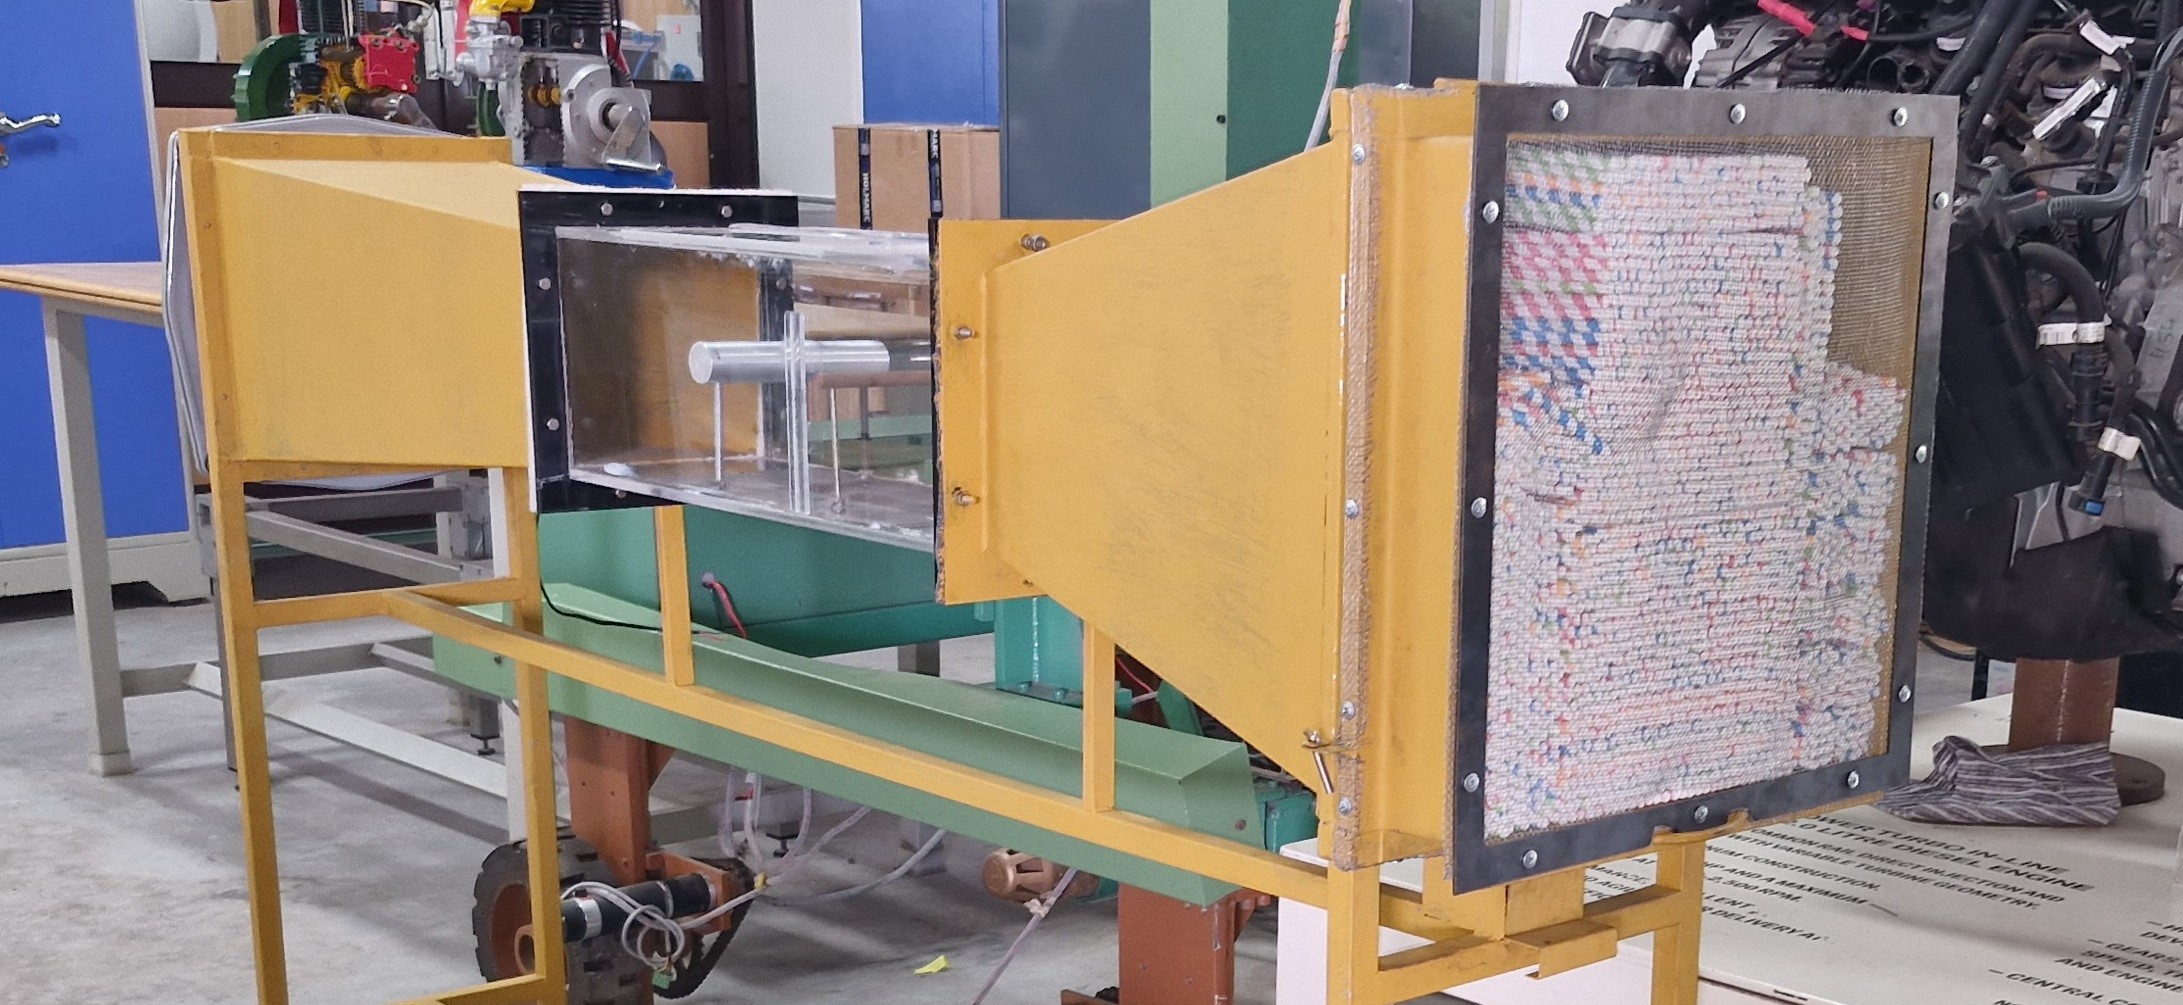
\includegraphics[width=0.9\linewidth]{gfx/windtunnel.jpg}
    \caption{Wind tunnel test rig.}
    \label{fig:wind_tunnel}
\end{figure}

\begin{itemize}

\item The air flows in the subsonic region and is incompressible.

\item The tunnel is assumed to be steady, with a uniform flow before the cylinder.

\item The Reynolds number will be chosen on the basis of typical flow conditions in the wind tunnel.

\end{itemize}
The following sections discuss the parts of the wind tunnel.
\subsection{Settling chamber}

The settling chamber is the first section of the wind tunnel. Its primary purpose is to stabilize the air flow and remove large turbulence before the air moves into the contraction section.

% \subsubsection{Purpose:}
% \begin{itemize}
% \item Reduce large-scale turbulence.

% \item Allow airflow to become more uniform and laminar before entering the contraction section.
% \end{itemize}
\subsubsection{Length calculations:}

The length of the settling chamber is usually between 0.25 to 4 times the width of the tunnel.  Width of the settling chamber (W$_{\text{settling}}$) is taken as 0.4 m. The length of the settling chamber (L$_{\text{settling}}$) should be between 0.1 m and 0.15 m and it is taken as 0.1 m  for better flow conditioning.


\subsection{Contraction Section}
The contraction section is used to accelerate the flow towards the test section while ensuring that the air flow remains smooth. This section converges the cross-sectional area, accelerating the air and increasing the velocity as it moves through the wind tunnel.
\begin{figure}[H]
    \centering
    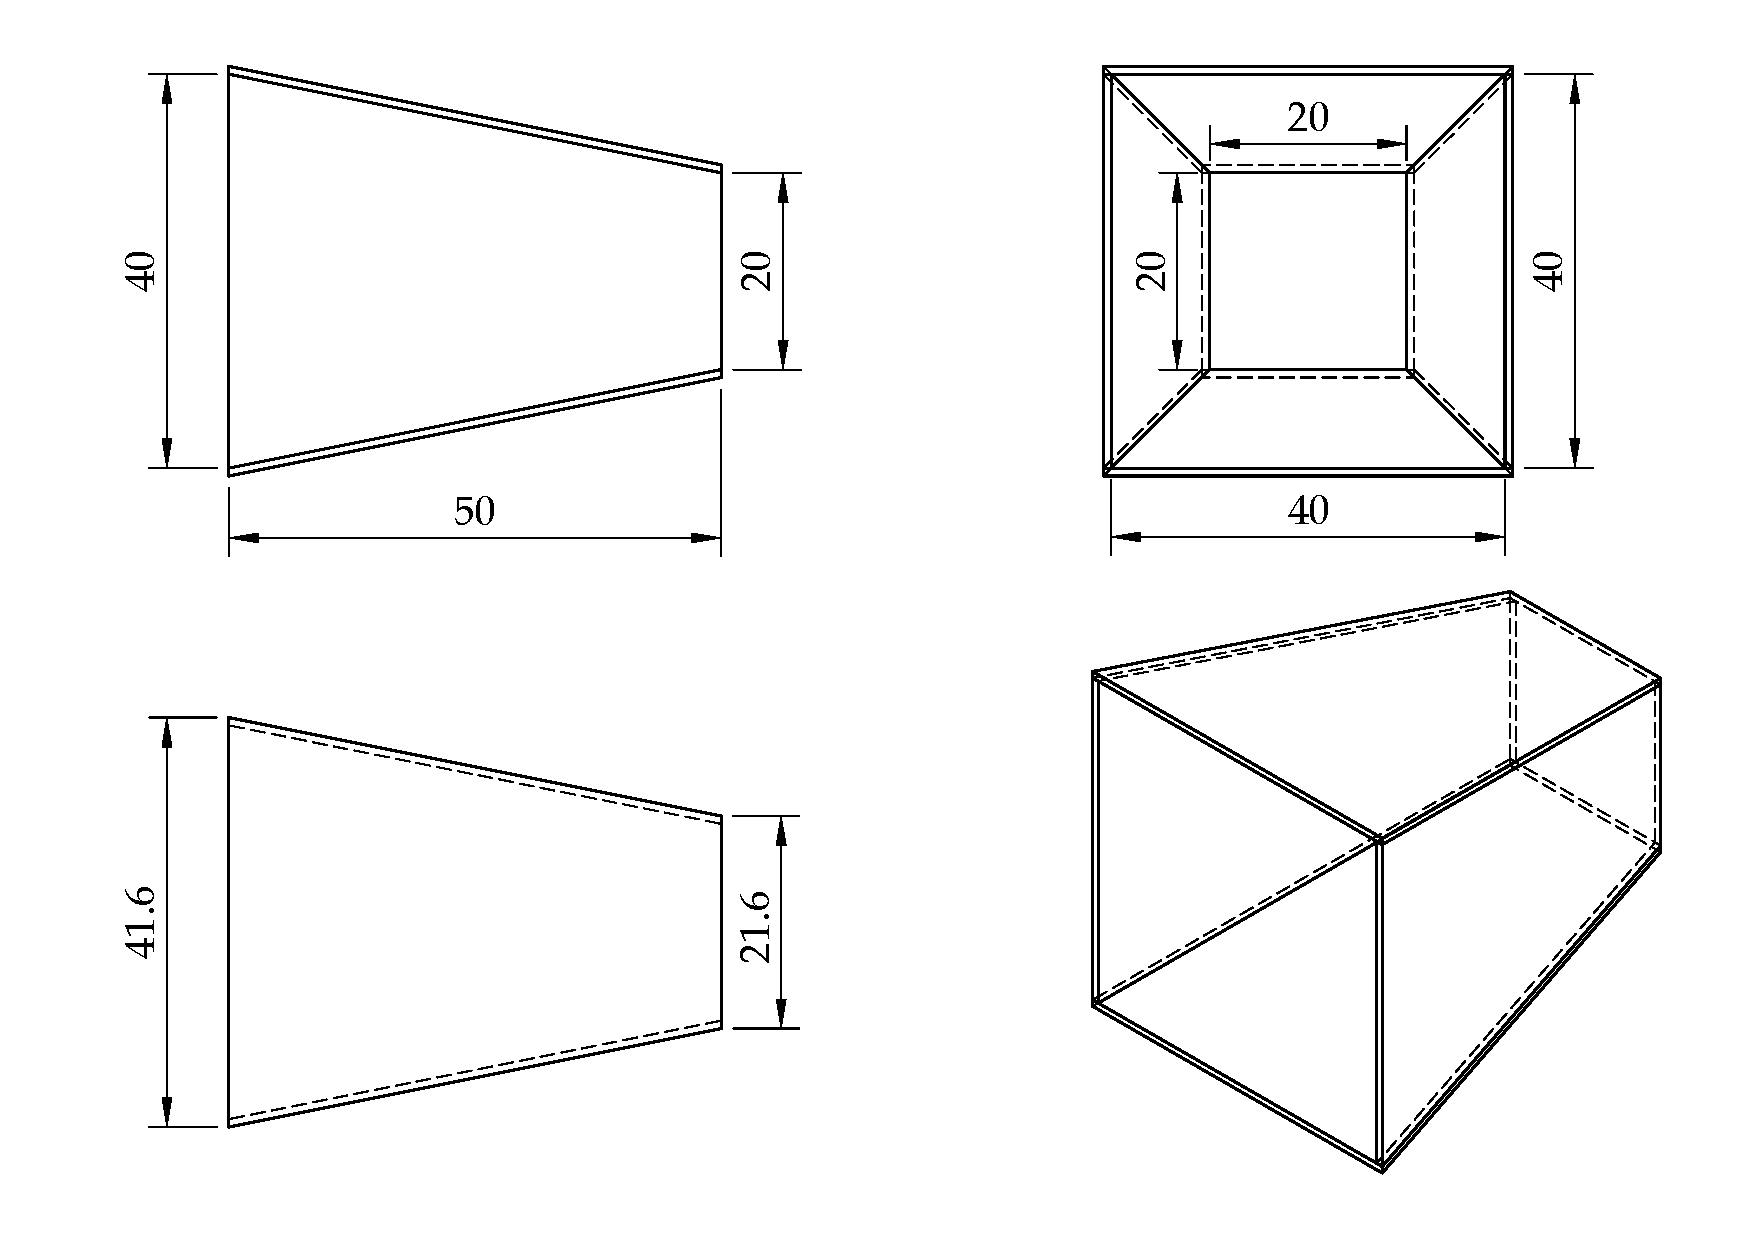
\includegraphics[width=\linewidth]{gfx/Convergent_section_wind_tunnel.pdf}
    \caption{Dimensions of converging section.}
    \label{fig:converge section}
\end{figure}

% \subsubsection{Purpose:}
% \begin{itemize}

% \item To accelerate the flow towards the test section.

% \item To ensure that the flow remains laminar and does not separate.
% \end{itemize}
%\subsubsection{Design parameters}
%\begin{itemize}

%\end{itemize}
\subsubsection{Design Parameters}
A typical contraction ratio (the ratio between the cross-sectional area of the inlet and the cross-sectional area of the test section) is 4:1 for laminar flow. This ensures that the air accelerates smoothly as it enters the test section. The height of the contraction section, H$_{\text{Contraction}}$ = 20 cm and the width of the contraction section, W$_{\text{Contraction}}$ = 20 cm. The length of the contraction section is typically 2 to 5 times the width of the test section. So, length of the contraction section, L$_{\text{Contraction}}$ = 0.5 m 
%\end{itemize}

\subsection{Test Section}
The object (solid cylinder) is placed in the test section and the vortex shedding and flow measurements are analyzed. The air flow for analysis should be uniform. The test section provides uniform airflow for analysis. The calibration of the bulb filament and the hot wire anemometer is performed in the test section. Vortex analysis is also performed in the test section.

\begin{figure}[H]
    \centering
    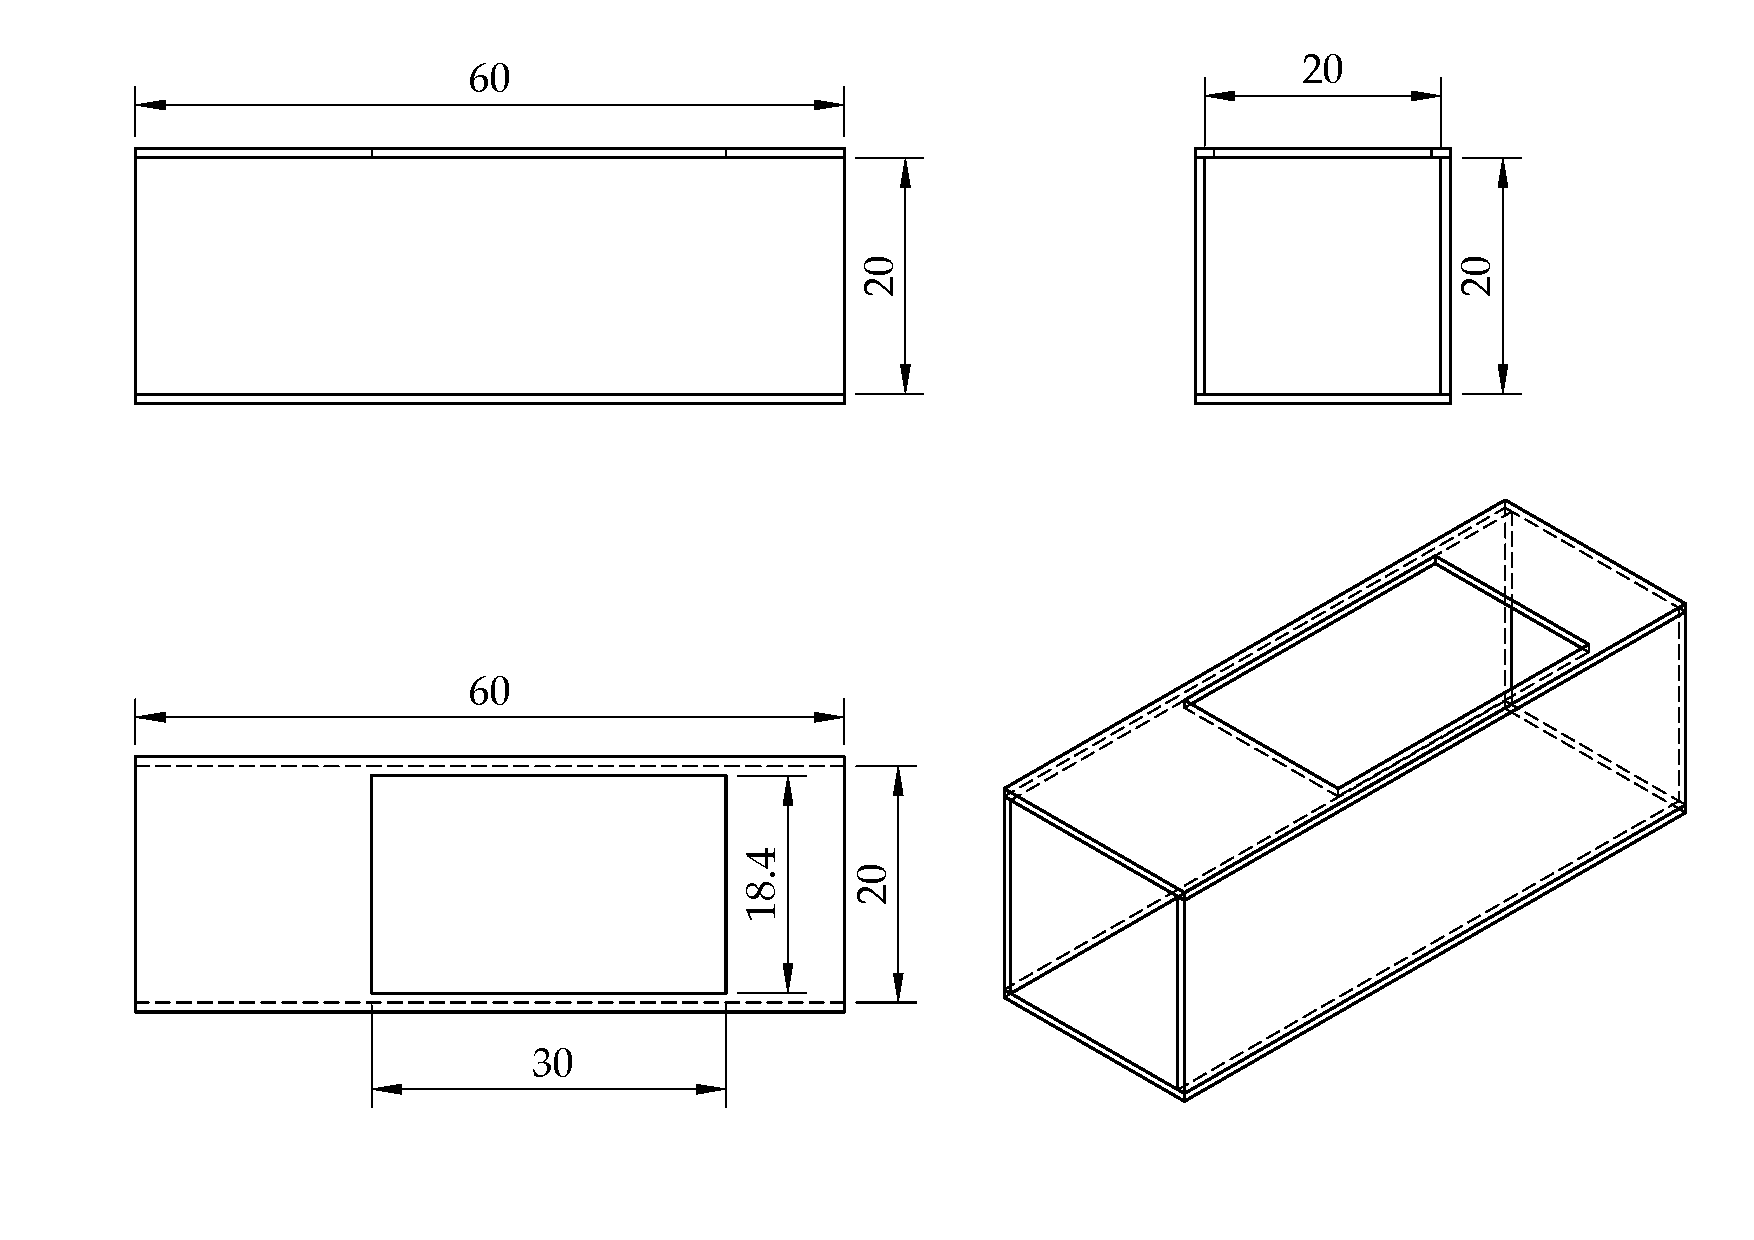
\includegraphics[width=\linewidth]{gfx/Wind_tunnel_test_section.pdf}
    \caption{Dimensions of the test section.}
    \label{fig:test section}
\end{figure}
%\subsubsection{Purpose:}
% \begin{itemize} 

% \item 

% \item Measure velocity changes with the tungsten bulb filament and hot wire anemometer.
% \end{itemize}
\subsubsection{Design parameters:}
%\begin{itemize}
The width and height of the test section should be at least 5–10 times the diameter of the cylinder. The diameter of the D-cylinder is 0.033 m (33 mm). So width and height of the test section is 
\begin{align}
W_{\text{test}} = 7 \times D = 7 \times\ 0.033 = 0.23 m\label{width test section}, \\
H_{\text{test}} = 7 \times D = 7 \times 0.033 = 0.23 m \label{height test section}.
\end{align}
So, the test section is designed to have a square cross section of side having 20~cm length.
%\end{itemize}
%\subsubsection{Length calculation:}
The length of the test section should be long enough to allow a fully developed flow before the air flow reaches the cylinder. The length is typically between 10 to 20 times the diameter of the test object (the cylinder) to allow for stable flow development. So, the length of the test section,
\begin{align}\label{length test section}
L_{\text{test}} = 18 \times D = 18 \times 0.033 =  0.6 m
\end{align}

\subsection{Diffuser Section}
The Diffuser Section is the final section of the wind tunnel, and its purpose is to slow down the airflow after the test section while minimizing turbulence. In this section, the airflow expands in the cross-sectional area, leading to a decrease in the velocity of the air, which helps to prevent any damage or instability in downstream equipment such as fans or flow measurement instruments. In addition, the diffuser allows the pressure to recover smoothly. The diffuser should have a gentle expansion to avoid turbulent separation. The cross-sectional area of the diffuser gradually increases, which reduces the velocity of the flow. The expansion ratio (the ratio of the inlet to the outlet area) is typically between 1.5:1 to 2:1 to ensure smooth deceleration without flow separation.
\begin{figure}[H]
    \centering
    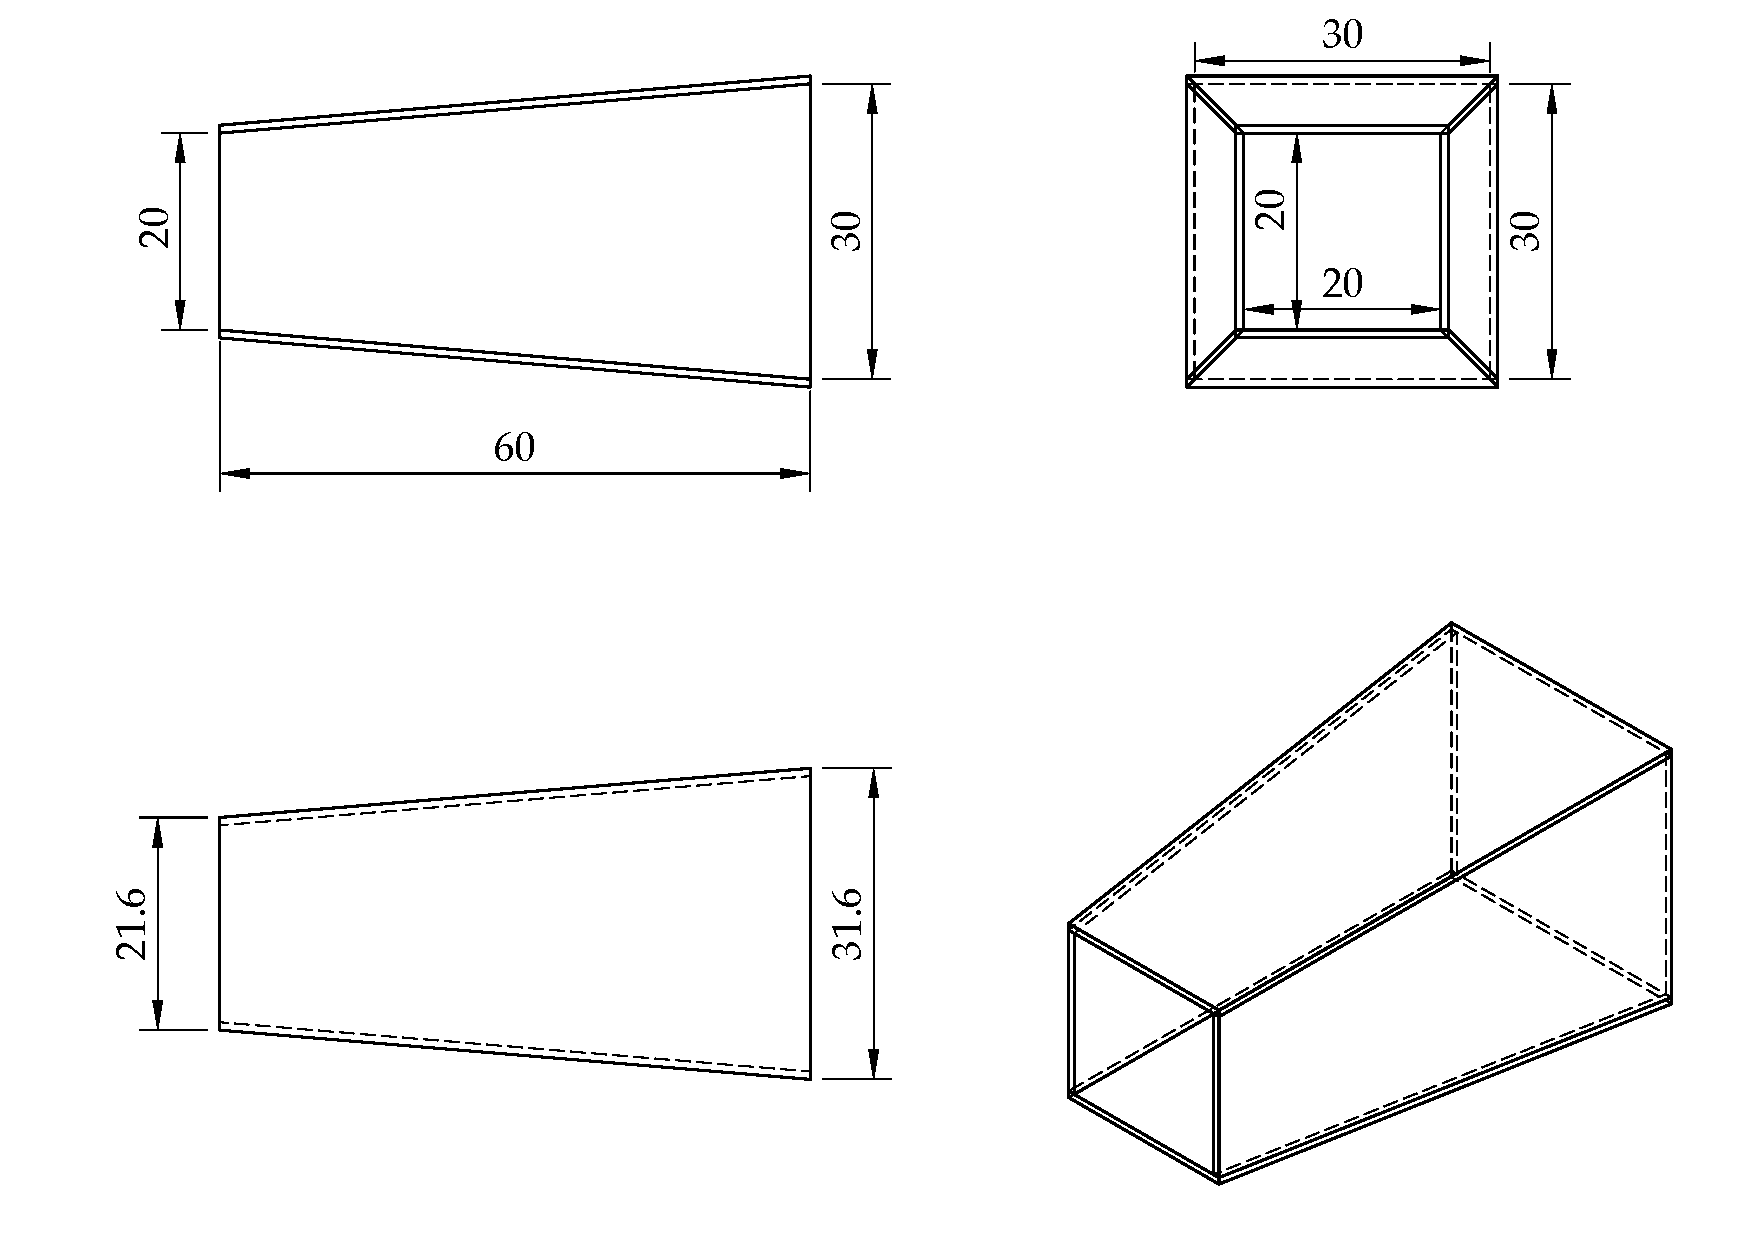
\includegraphics[width=\linewidth]{gfx/Divergent_section_for_wind_tunnel.pdf}
    \caption{Dimensions of diverging section.}
    \label{fig:diverge section}
\end{figure}
\subsubsection{Design parameters}
%The width and height of the diffuser section is designed in such a way that it expands relative to the test section.
The diffuser must also allow for the transition from the uniform flow of the test section to the slower flow at the exit of the tunnel. The cross section of the diffuser section near the test section should be equal to the cross section of the test section. It should gradually increase at the other end for smooth flow expansion.
%Since the width and height of the test section are decided to be 0.2 m, the diffuser section can be designed with the following dimensions:
So, the width (W$_{\text{diffuser}}$) and height (H${_\text{diffuser}}$) of the diffuser near the test section is 0.2~m and it is 0.4~m at the end. 
%Increase the width gradually from 0.2 m to a higher value, ensuring a smooth transition. Typically, the width may expand to 0.3 m at the end of the diffuser.
%Height : The height should also increase from 0.2 to 0.3 m, maintaining the ratio of the test section.Height of diffuser section = 0.3 m

Length of the diffuser should be long enough to allow the flow to gradually decelerate and the pressure to recover smoothly. The length is generally 2 to 5 times the width of the diffuser section. Since the diffuser width at the end is 0.3 m, the length of the diffuser is
\begin{align}
    L_{\text{Diffuser}}= 2 \times 0.3 = 0.6~m\nonumber
\end{align}
% L$_{\text{Diffuser section}}$ = 2 × W$_{\text{Diffuser section}}$ to 5 × w$_{\text{Diffuser section}}$

% Substituting the width:

% Length of diffuser section,

To design a gentle expansion, the ratio of the inlet area (of the test section) to the outlet area (of the diffuser) should be between 1.5:1 to 2:1. This would allow the air to decelerate without excessive turbulence.

\section{Hot Wire Filament}

When selecting a hot wire filament that is used in light bulbs or heating elements, it is essential to calculate its resistance, surface area and the maximum temperature at which the filament can operate safely. Below is a detailed breakdown of how to select the filament based on the provided information: The resistance of the filament and the operating temperature are calculated on the basis of material properties and filament dimensions. The resistance $R$ of the filament can be estimated using the equation
\begin{equation}\label{eq:resistance}
R = \rho_w \frac{L_w}{A_w},
\end{equation}
where $\rho_w$ is the resistivity of tungsten ($5.6 \times 10^{-8}\Omega m$), $L_w$ is the length of the filament ($4~mm$) and $A_w$ is the cross-sectional area of the filament ($7.853 \times 10^{-12}~m^2$). 
%calculated using the diameter \( d = 0.1 \, mm = 0.1 \times 10^{-3} \, m \).
Substituting the values in Eq.~(\ref{eq:resistance}), the resistance $R$ of the filament is estimated to be $0.03\Omega$. The maximum operating temperature of the filament is determined using the energy balance equation
\begin{equation}\label{eq:energy balance}
I^2 R = h A_w (T_{\text{wire}} - T),    
\end{equation}
where $I$ is the current, $R$ is the resistance of the wire (Eq.~(\ref{eq:resistance})), $h$ is the heat transfer coefficient ($10~W/m^2K$), $A$ is the surface area of the filament ($1.256 \times 10^{-5}~m^2$) and $T$ is the ambient temperature ($32^\circ C$). Substituting the above values in Eq.~(\ref{eq:energy balance}), the maximum filament temperature $T_{\text{wire}}$ can be estimated to be $300^\circ C$. Thus, the tungsten filament will operate at a maximum temperature of approximately 300 ° C.

% \section*{Design Parameters}
% \begin{itemize}
%     \item \textbf{Material}: Tungsten
%     \item \textbf{Filament Length}: 4 mm
%     \item \textbf{Filament Diameter}: 0.1 mm
%     \item \textbf{Resistance}: 0.03 $\Omega$
%     \item \textbf{Cross-sectional Area}: \( 7.853 \times 10^{-12} \, \text{m}^2 \)
%     \item \textbf{Surface Area}: \( 1.256 \times 10^{-5} \, \text{m}^2 \)
%     \item \textbf{Ambient Temperature}: 32 °C
%     \item \textbf{Maximum Filament Temperature}: 300 °C
% \end{itemize}


\section{Fan Power calculation}
This section provides a detailed calculation to determine the required fan power for a wind tunnel with the dimensions described in the previous section and the flow conditions. 
%The calculations include the area, velocity, pressure drop across various sections and the final fan power required to maintain a test section velocity of 20 m/s.

\subsection{Area Calculations}
%The cross-sectional area of each section is calculated as
Area of the contraction section
\begin{equation}\label{area of contraction}
A_{\text{contraction}} = W_{\text{contraction}}\cdot H_{\text{contraction}} = 0.4\cdot 0.4 = 0.16~\text{m$^2$},
\end{equation}
area of the test section
\begin{equation}\label{area of test}
    A_{\text{test}} = W_{\text{test}}\cdot H_{\text{test}} = 0.2\cdot 0.2 = 0.04~\text{m$^2$}
\end{equation}  
and the area of the diffuser section
\begin{equation}\label{area of diffuser}
    A_{\text{diffuser}} = W_{\text{diffuser}} \cdot H_{\text{diffuser}} = 0.3 \cdot 0.3 = 0.09 ~\text{m}^2.
\end{equation}


% \begin{align}
% A_{\text{settling}} &= W_{\text{settling}} \cdot H_{\text{settling}} = 0.4 \, \text{m} \cdot 0.4 \, \text{m} = 0.16 \, \text{m}^2. \\
% A_{\text{test}} &= W_{\text{test}} \cdot H_{\text{test}} = 0.2 \, \text{m} \cdot 0.2 \, \text{m} = 0.04 \, \text{m}^2. \\
% A_{\text{diffuser}} &= W_{\text{diffuser}} \cdot H_{\text{diffuser}} = 0.3 \, \text{m} \cdot 0.3 \, \text{m} = 0.09 \, \text{m}^2.
% \end{align}

\subsection{Flow Rate Calculation}
The air flow rate $Q$ in the test section is calculated as
\begin{flalign}\label{air flow rate}
Q = A_{\text{test}}\cdot V_m = 0.04\cdot 20 = 0.8~m^3/s, 
\end{flalign}
where $A_{\text{test}}$ is the area of the test section (Eq.~(\ref{area of test})) and $V_m$ is the maximum air flow velocity which is assumed as 20~m/s.
%So, the air flow rate in the test section, $Q$ = 0.8~m$^3$/s.    

\subsection{Pressure Drop Calculations}

%\paragraph{(a) Settling Chamber Pressure Drop (Straws)}
The pressure drop in the settling chamber is given by
\begin{equation}\label{pressure drop settling}
    \Delta P_{\text{settling}} = k_{\text{settling}} \cdot \frac{\rho V_{\text{settling}}^2}{2}, 
\end{equation}
where $k_{\text{settling}}$ is the loss factor (= 1.5), $\rho$ is the density of the air and $V_{\text{settling}}$ is the velocity of the air flow in the settling chamber. The air and settling chamber contact area includes the straw area that is placed to obtain uniform air flow. The contact area is given by
\begin{align}\label{area of straw}
A_{\text{straws}} = A_{\text{contraction}}\cdot \text{porosity factor} = 0.16 \cdot 0.8 = 0.128~\text{m}^2.
\end{align}
From Eqs.~(\ref{air flow rate}) and (\ref{area of straw}), the velocity of the air at the settling chamber is 
\begin{align}\label{air velocity in settling}
    V_{\text{settling}} = \frac{Q}{A_{\text{straws}}} = \frac{0.8}{0.128} = 6.25  \text{m/s}.
\end{align}
Substituting Eq.~(\ref{air velocity in settling}) in Eq.~(\ref{pressure drop settling}), the pressure drop in the settling chamber is calculated as
\begin{align}\label{pressure drop settling value}
    \Delta P_{\text{settling}} &= 1.5 \cdot \frac{1.21 \cdot 6.25^2}{2} = 35.16~\text{Pa}.
\end{align}
%\paragraph{(b) Contraction Section Pressure Drop}

The pressure drop in the contraction section is given by
\begin{align}
\Delta P_{\text{contraction}} = k_{\text{contraction}} \cdot \frac{\rho V_{\text{m}}^2}{2},
\end{align}
where $k_{\text{contraction}}$ is the loss factor (= 0.1), $V_{\text{m}}$ is the maximum velocity of the air in the test section. Substituting all the values, the pressure drop in the contraction section is calculated as
\begin{align}\label{pressure drop contraction value}
\Delta P_{\text{contraction}} = 0.1 \cdot \frac{1.21 \cdot 20^2}{2} = 24~\text{Pa}.
\end{align}
%\paragraph{(c) Test Section Pressure Drop}
%\begin{align}
%\section*{Pressure Drop in the Test Section}

The pressure drop in the test section is given by
\begin{align}\label{pressure drop test section}
    \Delta P_{\text{test}} = \frac{1}{2} \rho V_{\text{m}}^2 f_f \frac{L_{\text{test}}}{D_h},
\end{align}
where $f_f$ is the friction factor (= 0.02), $L_{\text{test}}$ is the length of the test section (Eq.~(\ref{length test section})) and $D_h$ is the hydraulic diameter given by
\begin{equation}\label{hydraulic diameter equation}
    D_h = \frac{4 \cdot A_{\text{test}}}{P_{\text{test}}},
\end{equation}
where $A_{\text{test}}$ is the area of cross section of the test section (Eq.~(\ref{area of test})). $P_{\text{test}}$ is the wetted perimeter of the test section given by
\begin{equation}\label{perimeter of the test}
    P_{\text{test}} = 2 \cdot (W_{\text{test}} + H_{\text{test}}) = 2 \cdot (0.2 + 0.2) = 0.8~\text{m},
\end{equation}
where $W_{\text{test}}$ is the width of the test section (Eq.~(\ref{width test section})) and $H_{\text{test}}$ is the height of the test section (Eq.~(\ref{height test section})).
% \begin{itemize}
%     \item \(A\) is the cross-sectional area of the rectangle: \(A_{\text{test}} = W_{\text{test}} \cdot H_{\text{test}}\)
%     \item \(P\) is the wetted perimeter of the rectangle: \(P_{\text{test}} = 2 \cdot (W_{\text{test}} + H_{\text{test}})\)
% \end{itemize}
Substituting Eqs.~(\ref{area of test}) and (\ref{perimeter of the test}) in Eq.~(\ref{hydraulic diameter equation}), the hydraulic diameter of the test section is calculated as
% \[
% A_{\text{test}} = W_{\text{test}} \cdot H_{\text{test}} = 0.2 \cdot 0.2 = 0.04 \, \text{m}^2
% \]
% \[
% P = 2 \cdot (W_{\text{test}} + H_{\text{test}}) = 2 \cdot (0.2 + 0.2) = 0.8 \, \text{m}
% \]
%Now, calculate \(D_h\):
\begin{align}\label{hydraulic diameter}
    D_h = \frac{4 \cdot 0.04}{0.8} = 0.2~\text{m}
\end{align} 
% Thus, the hydraulic diameter is:
% \[
% D_h = 0.2 \, \text{m}
% \]
% where the air density (\(\rho\)) is 1.17 kg/m³, the velocity (\(V\)) is 20 m/s, the friction factor (\(f_L\)) is 0.02, the length of the test section (\(L\)) is 0.6 m, and the hydraulic diameter (\(D_h\)) is 0.2 m.
Substituting Eqs.~(\ref{length test section}), (\ref{hydraulic diameter}) in Eq.~(\ref{pressure drop test section}), the pressure drop in the test section is calculated as
\begin{align}\label{pressure drop test section value}
    \Delta P_{\text{test}} = \frac{1}{2} (1.21) (20)^2 (0.02) \frac{0.6}{0.2} = 14.4~\text{Pa}
\end{align}


% \[
% \Delta P_{\text{test}} = 240 \times 0.02 \times 3 = 14.4 \, ~\text{Pa}
% \]

% Thus, the pressure drop in the test section is:

% \[
% \boxed{\Delta P_{\text{test}} = 14.4 \, ~\text{Pa}}
% \]

%\paragraph{(d) Diffuser Section Pressure Drop}
The pressure drop in the diffuser section is given by
\begin{align}\label{pressure drop diffuser value}
\Delta P_{\text{diffuser}} &= k_{\text{diffuser}} \times \frac{\rho V_{\text{m}}^2}{2} = 0.2 \times \frac{1.21 \times 20^2}{2} = 48~\text{Pa}, 
\end{align}
where $k_{\text{diff}}$ is the loss factor in the diffuser (= 0.2).
% \begin{align}
% \Delta P_{\text{diff}} &= 0.2 \times \frac{1.2 \times 20^2}{2} = 48 \, ~\text{Pa} \nonumber.
% \end{align}
%\paragraph{(e) Total Pressure Drop}
From Eqs.~(\ref{pressure drop settling value}), (\ref{pressure drop contraction value}), (\ref{pressure drop test section value}) and (\ref{pressure drop diffuser value}), the total pressure drop in the wind tunnel is 
\begin{equation}
\begin{aligned}\label{pressure drop total value}
\Delta P_{\text{total}} &= \Delta P_{\text{settling}} + \Delta P_{\text{contraction}} + \Delta P_{\text{test}} + \Delta P_{\text{diffuser}}, \\
\Delta P_{\text{total}} &= 35.16 + 24 + 2 + 48 = 109.16~\text{Pa}.
\end{aligned}
\end{equation}

%\subsection{Power Calculation}
The required power of the suction fan can be calculated as
\begin{align}
P_{\text{fan}} &= \frac{\Delta P_{\text{total}} \cdot Q}{\eta},
\end{align}
where $\Delta P_{\text{total}}$ is the total pressure drop in the wind tunnel (Eq.~(\ref{pressure drop total value})), $Q$ is the air flow rate in the wind tunnel (Eq.~(\ref{air flow rate})) and $\eta$ is the efficiency (= 0.7). Substituting above values, the power of the suction fan is calculated as
\begin{align}
P_{\text{fan}} = \frac{109.16 \times 0.8}{0.7} = 124.7~\text{W} \approx 0.167~\text{HP}.
\end{align}

% \subsection*{ Verification with 0.5 HP Fan}
% \begin{align}
% P_{\text{available}} &= 0.5 \, \text{HP} = 373 \, \text{W}.\nonumber \\
% P_{\text{available}} &\gg P_{\text{fan}}, \text{indicating the fan is sufficient.}\nonumber
% \end{align}


% \begin{itemize}
%     \item \textbf{Flow Rate:} \( 0.8 \, \text{m}^3/\text{s} \).
%     \item \textbf{Total Pressure Drop:} \( 109.16 \, \text{Pa} \).
%     \item \textbf{Required Fan Power:} \( 0.167 \, \text{HP} \).
%     \item \textbf{Available Fan Power:} \( 0.5 \, \text{HP} \).
% \end{itemize}
For an air flow velocity of $20~m/s$, the required power of the suction fan is approximately $0.167~HP$. In this project, the power of the suction fan used is $0.5~HP$, which is sufficient to carry out this project.
\newpage
\section{Design Summary of the wind tunnel}
\begin{table}[h]
    \centering
    \caption{Design summary of wind tunnel.}
    \begin{tabularx}{\textwidth}{|>{\centering\arraybackslash}X|>{\centering\arraybackslash}X|>{\centering\arraybackslash}X|>{\centering\arraybackslash}X|>{\centering\arraybackslash}X|}
    \toprule
       \textbf{Section} & \textbf{Length (m)} & \textbf{Length (m)} & \textbf{Length (m)} & \textbf{Purpose} \\
         \midrule
        Settling chamber & 0.1 & 0.4 & 0.4 & To remove turbulence and stabilize the flow\\ \hline
        Converging section & 0.5 & 0.2 & 0.2 & To accelerate the flow towards the test section \\ \hline
         Test section & 0.6 & 0.2 & 0.2 & To perform testing with uniform flow around the cylinder \\ \hline
        Diffusing section & 0.6 & 0.3 & 0.3 & To decelerate the flow after the test section\\ \hline
        Fan (Suction type - Power 0.5 hp) & -  & 0.3 & 0.3 & To house the fan and expel air from the system \\
         \bottomrule
    \end{tabularx}  
    \label{tab:des_summ_windtunnel}
    
    The suction-type fan, with a power of 0.5 HP and dimensions of 0.3 m × 0.3 m, is designed to accommodate the fan mechanism and efficiently expel air from the system.
\end{table}



\chapter{Experimental procedure}\label{ch:procedure}
Procedure of the experiment...
\chapter{Results and discussions}\label{ch:results}
In this chapter, the vortex analysis of air flow over a solid cylinder using a constant-current hot wire anemometer is discussed.
The vortex analysis is performed at a distance of $D$, $2~D$ and $4~D$ from the cylinder, where $D$ is the diameter of the cylinder. The analysis is also performed at a distance of $0.5~D$ above the cylinder at all the points mentioned above. The air flow is kept at a pitot tube pressure of $1~Pa$, $2~Pa$, $3~Pa$ and $4~Pa$. The results are discussed in the following sections.

\section{Vortex analysis at distance \texorpdfstring{$x=D$}~~from the cylinder}
In this section, the vortex analysis of the flow is done by keeping the hot wire anemometer at a distance of $D$ from the center of the cylinder. Further, the probe is moved to a height of $0.5~D$ above the center of the cylinder, and the same analysis is performed. 
\subsection{Vortex analysis at the center of the cylinder}


\begin{figure}[h]
    \centering
    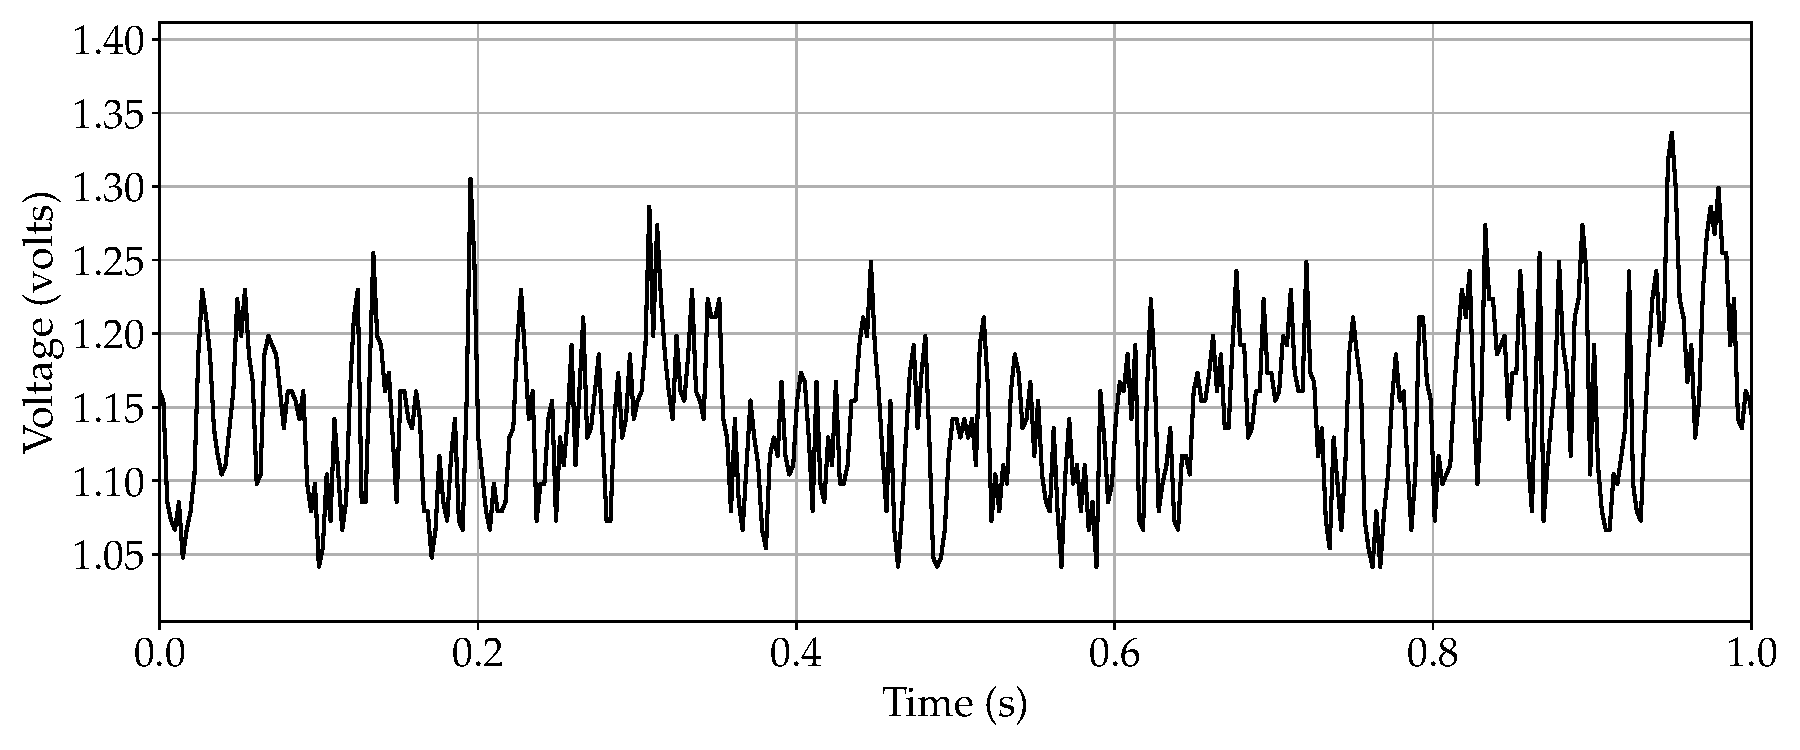
\includegraphics[width=\linewidth]{gfx/voltage_vs_time_for_1Pa_1s.pdf}
    \caption{The variation of voltage with time for a flow having differential pressure of $1~Pa$ for sensor placed at a distance of $D$ from the cylinder}
    \label{fig:vortex_D_1Pa}
\end{figure}

The solid cylinder is kept at a distance of $0.20~m$ from the left end of the test section. The speed of the suction fan is varied from an equivalent differential pressure of $1~Pa$, $2~Pa$, $3~Pa$ and $4~Pa$ using an auto transformer. The output of the hot wire anemometer is recorded in the PC Oscilloscope for a time of $10~s$ for all flow pressures. The voltage variation with time for a flow having differential pressure of $1~Pa$ (between $0~\text{to}~1~s$) is shown in Fig.~\ref{fig:vortex_D_1Pa}.

The interest is to find the velocity fluctuation in the test section due to the presence of a solid cylinder. The voltage output from the oscilloscope is converted to velocity using the calibration equation (see Eq.~(\ref{eq:calib_eqn_hwa})). The corresponding velocity fluctuation with time is shown in Fig.~\ref{fig:vortex_D_1Pa_vel}.

\begin{figure}
    \centering
    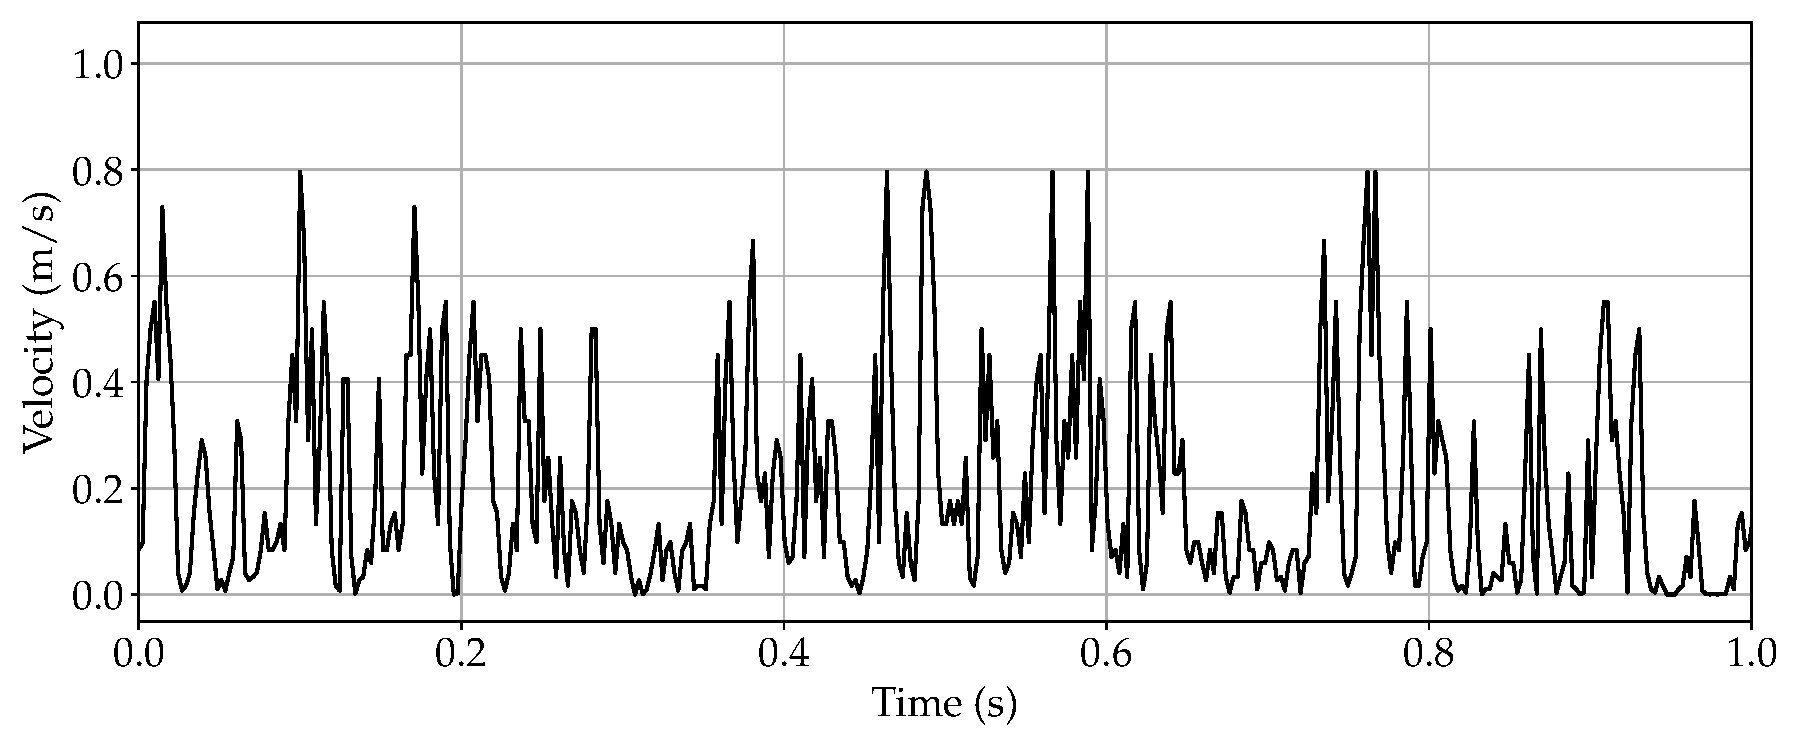
\includegraphics[width=\linewidth]{gfx/velocity_vs_time_for_1Pa_1s.pdf}
    \caption{The variation of velocity with time for a flow having differential pressure of $1~Pa$ for sensor placed at a distance of $D$ from the cylinder}
    \label{fig:vortex_D_1Pa_vel}
\end{figure}
The fluctuation in flow velocity is due to the occurrence of vortices when the flow is obstructed by the solid cylinder. Here, since the velocity varies with time, it can be assumed to be a function of time. That is,
\begin{equation}
    v = v(t).
\end{equation}
Further, the frequency of the vortex can be found by transforming the velocity from temporal domain ($t$) to frequency domain ($\omega$) using the Fourier transform pairs given by

\begin{equation}\label{eq:forward fourier}
        \Hat{V}(\omega) = \frac{1}{2\pi}\int^{\infty}_{-\infty}v(t)e^{-i\omega t}dt
\end{equation}
\begin{equation}\label{eq:backward fourier}
        v(t) = \int^{\infty}_{-\infty}\Hat{V}(\omega)\mathbf{e}^{i\omega t}d\omega
\end{equation}
where $\Hat{V}$ is the transformed velocity and $\omega$ is the frequency in $rad/s$ ($=2\pi f$, f - frequency in $Hz$). The velocity variation is transformed using Eq.~\ref{eq:forward fourier} and resulting frequency variation of velocity spectral density for flow having differential pressure of $1~Pa$ (scaled to 0~$Hz$ to $100~Hz$) is shown in Fig.~\ref{fig:vel_freq_1Pa}.
\begin{figure}
    \centering
    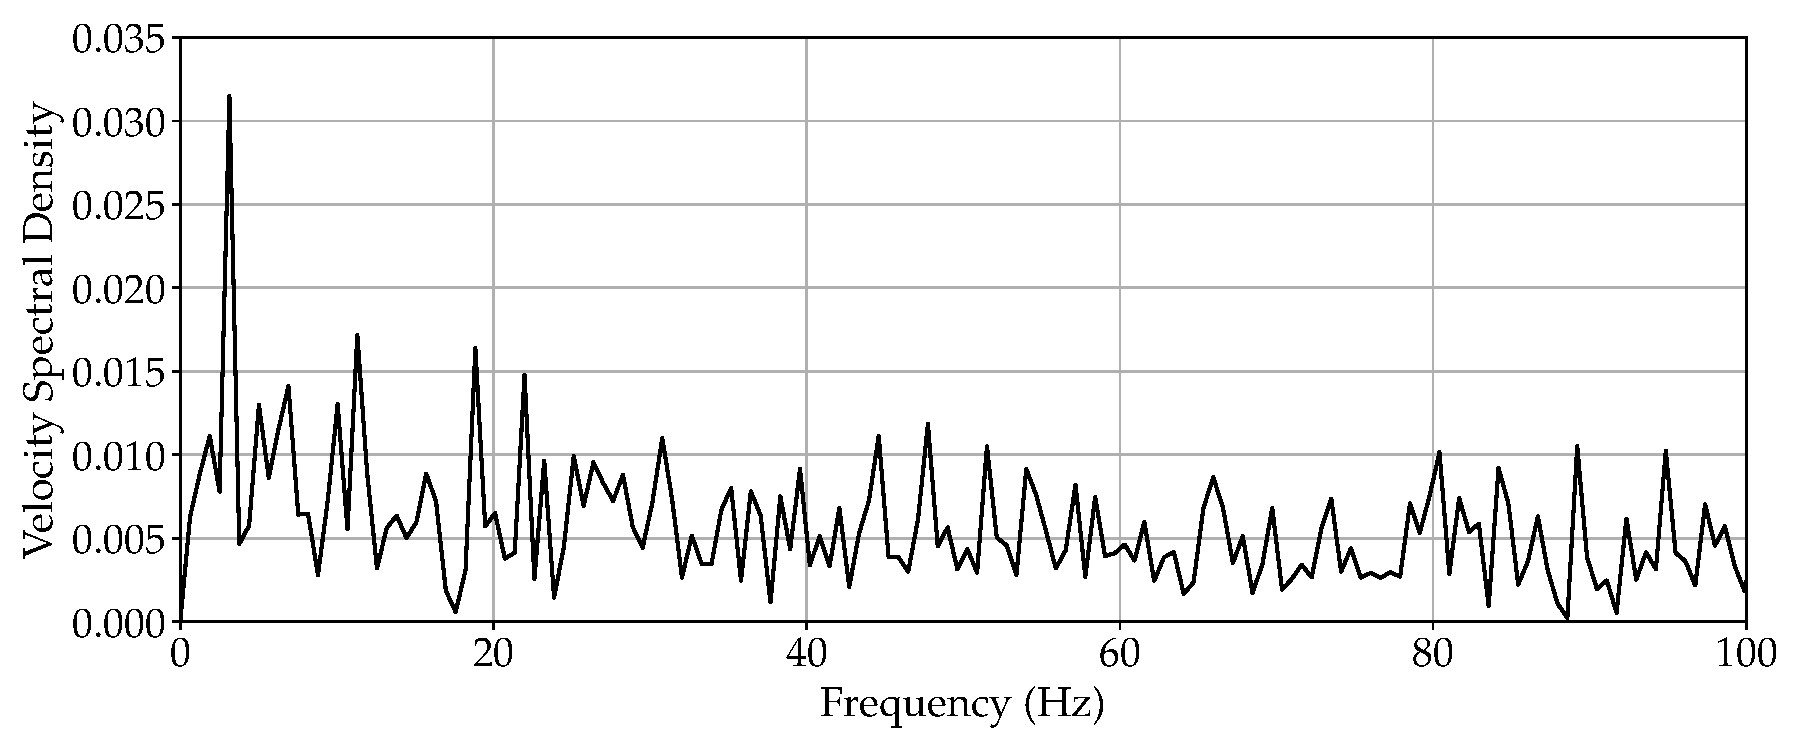
\includegraphics[width=\linewidth]{gfx/FFT_vel_1Pa.pdf}
    \caption{Frequency spectrum of velocity.}
    \label{fig:vel_freq_1Pa}
\end{figure}
In this figure, it can be seen that the velocity spectrum peaks at many frequencies. The maximum peak occurs at a frequency of about $3.14~Hz$, which corresponds to the frequency of the vortex. Similar frequency peaks are also found in other flow pressures of $2~Pa$, $3~Pa$ and $4~Pa$. Eq.~(\ref{eq:press_vel equation}) can be used to find the velocity corresponding to the flow pressure. The Reynolds number for the flow can be calculated using
\begin{equation}\label{eq:reynolds number}
    Re = \frac{\rho U D}{\mu},
\end{equation}
where $\rho$ is the density of air (1.17~$kg/m^3$), $U$ is the flow velocity in $m/s$, $D$ is the diameter of the solid cylinder ($0.033~m$) and $\mu$ is the dynamic viscosity of air ($1.87 \times 10^{-5}~kg/m\cdot s$). A comparison of velocity spectral density with frequency for all flow velocities (written in terms of Reynolds number) is shown in Fig.~\ref{fig:surface_x_D_y_0}.
\begin{figure}
    \centering
    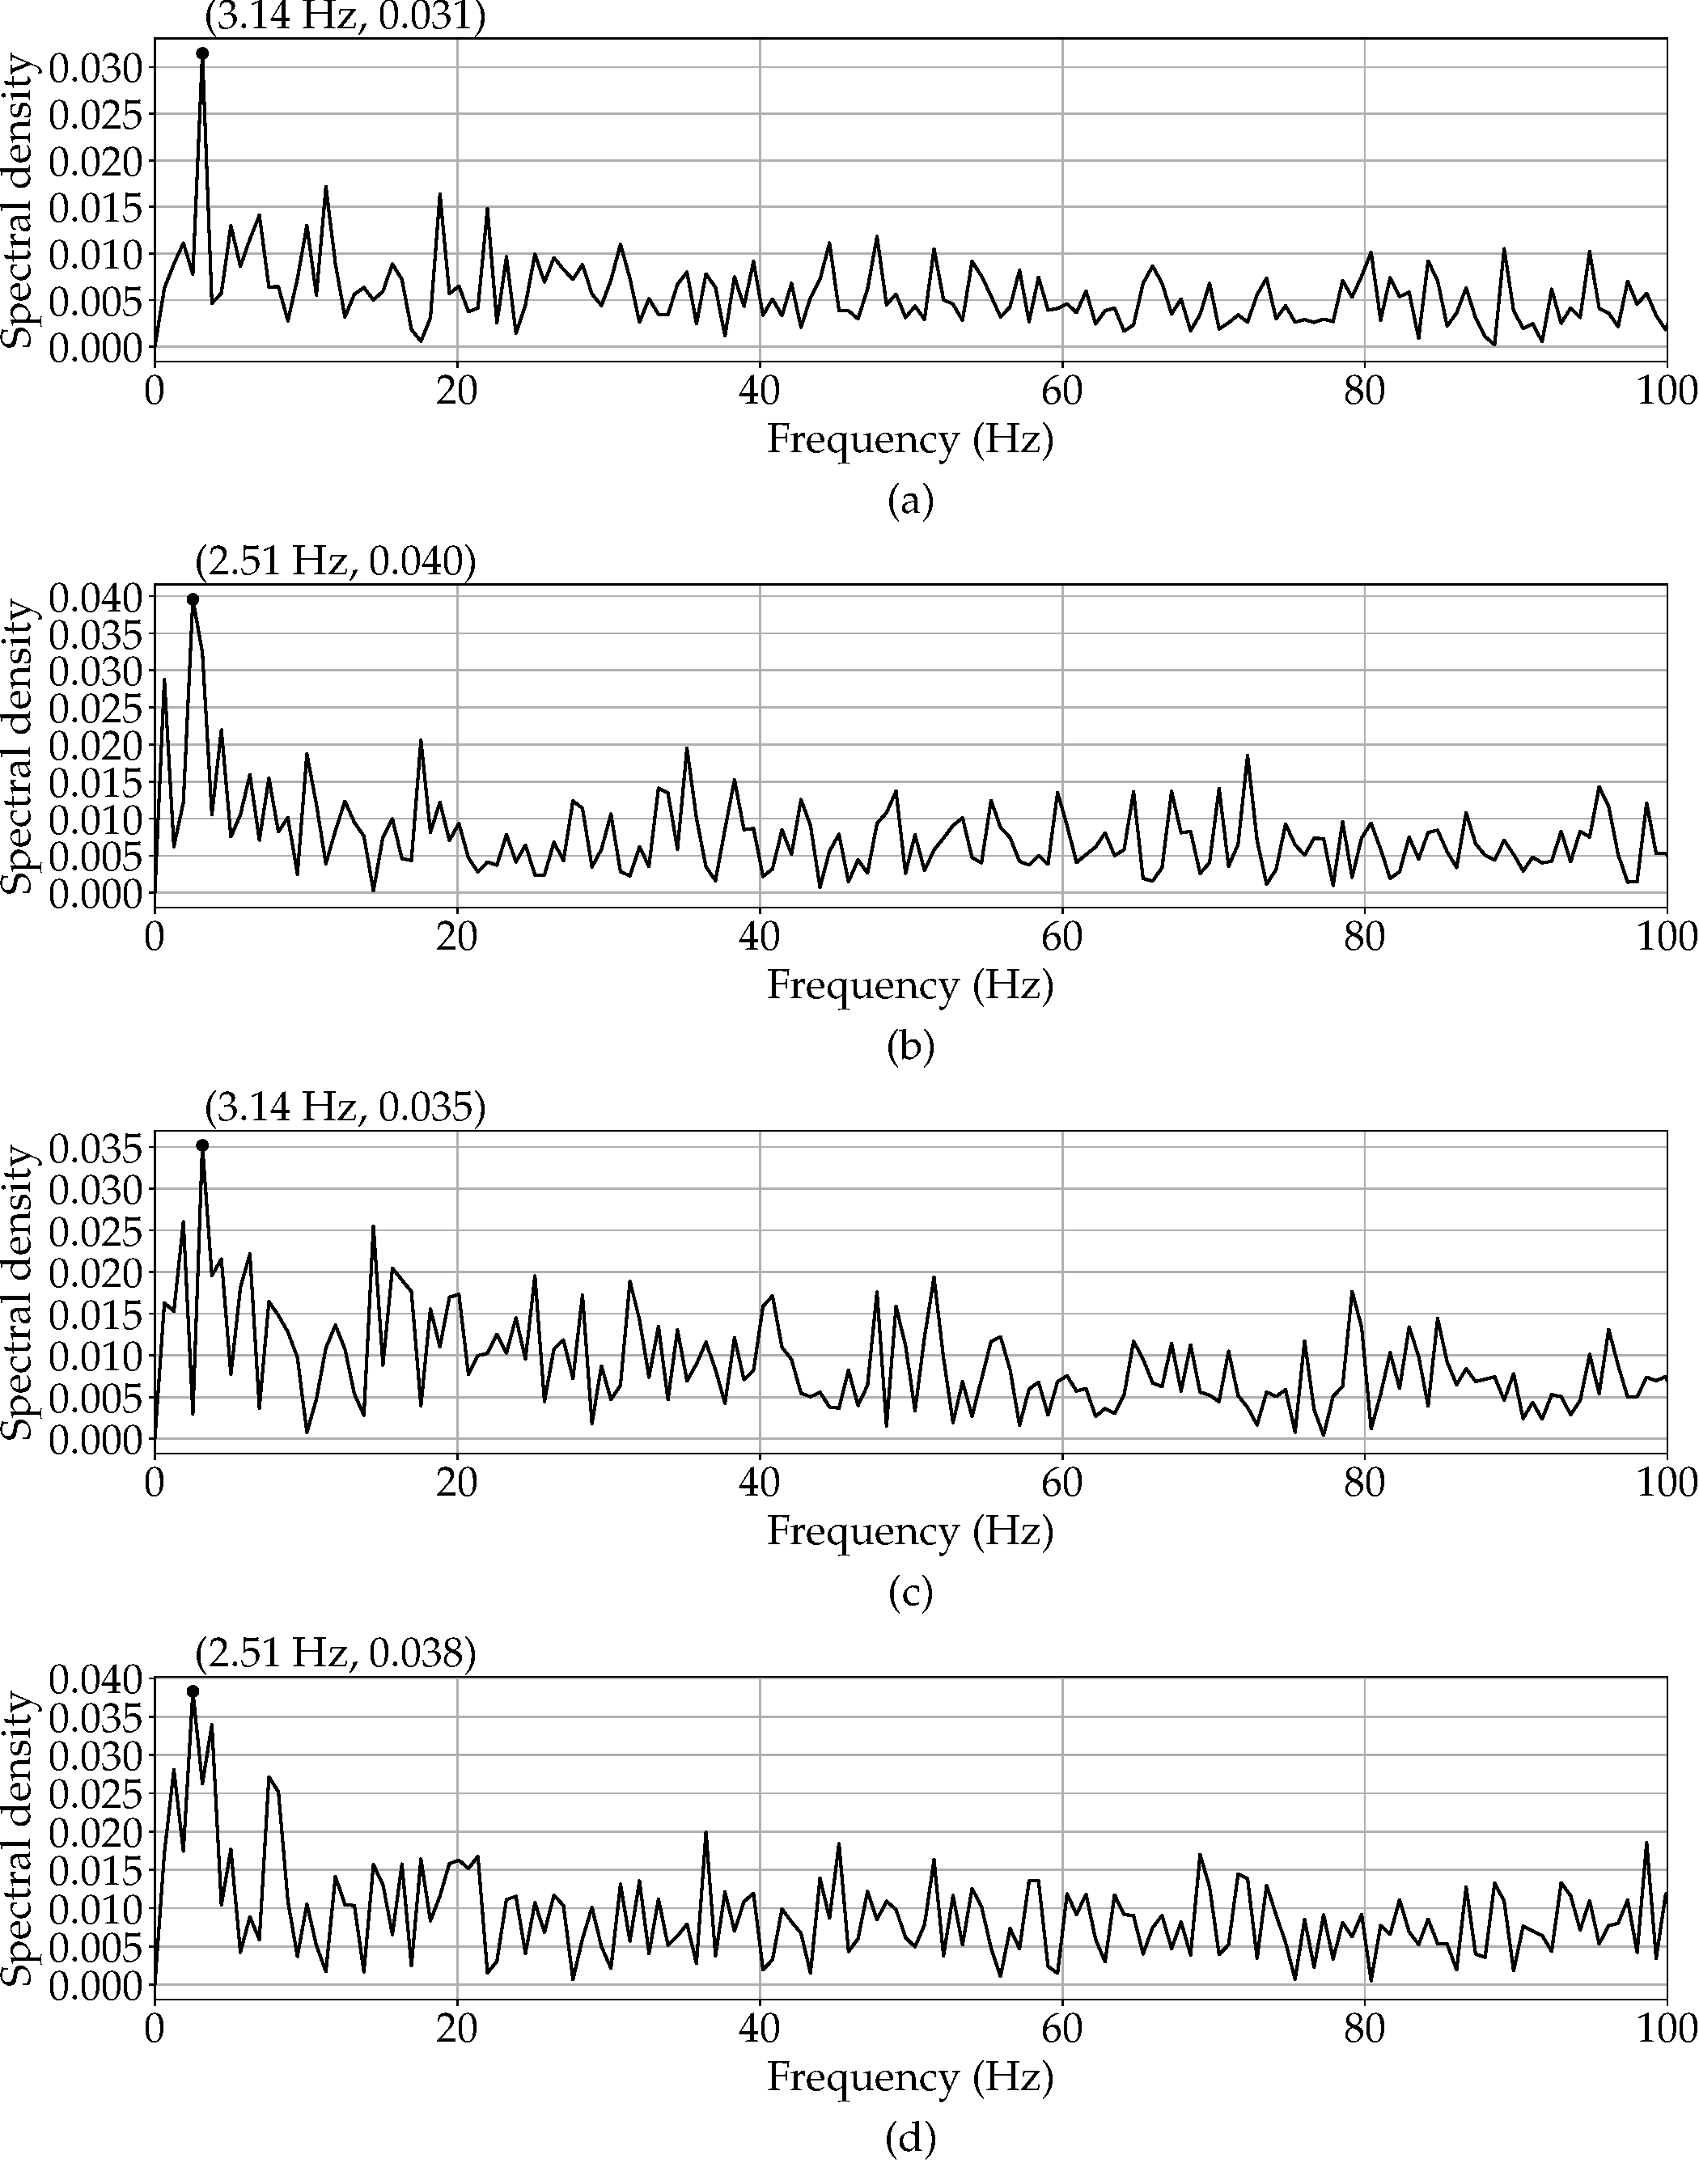
\includegraphics[width=\linewidth]{gfx/FFT_all_freq_x_D_y_0.pdf}
    \caption{Frequency spectral density of velocity for flow Reynolds number (a)~2699, (b)~3818, (c)~4676 and (d)~5399 at a distance of $D$ from the center of the cylinder.}
    \label{fig:surface_x_D_y_0}
\end{figure}

It can be seen in Fig.~\ref{fig:surface_x_D_y_0} that at each flow velocity, the peak frequency is different. This is due to the difference in the formation of the vortex at each velocity. At Reynolds numbers 2699 and 4676, the maximum peak occurs at a frequency of 3.14~Hz and at Reynolds numbers 3818 and 5399, the peak is at 2.51~Hz. The Reynolds number is the ratio of inertial forces to viscous forces. It describes whether the flow is laminar or turbulent. Similarly, the Strouhal number ($St$) is the ratio of oscillatory inertial forces to steady inertial force. It describes the relationship between an unsteady phenomenon (vortex shedding) and flow velocity. The Strouhal number is defined as
\begin{equation}\label{strouhal number}
    St = \frac{f\cdot D}{U},
\end{equation}
where $f$ is the frequency of the vortex in $Hz$, $D$ is the diameter of the solid cylinder and $U$ is the flow velocity. Assuming that the peak frequency in Fig.~\ref{fig:surface_x_D_y_0} dominates the entire spectrum, the peak frequency for all flows is used to calculate the Strouhal number. The two non-dimensional numbers (Reynolds number and Strouhal number) are plotted against each other in Fig.~\ref{fig:st_vs_re_x_D_y_0}. 
\begin{figure}
    \centering
    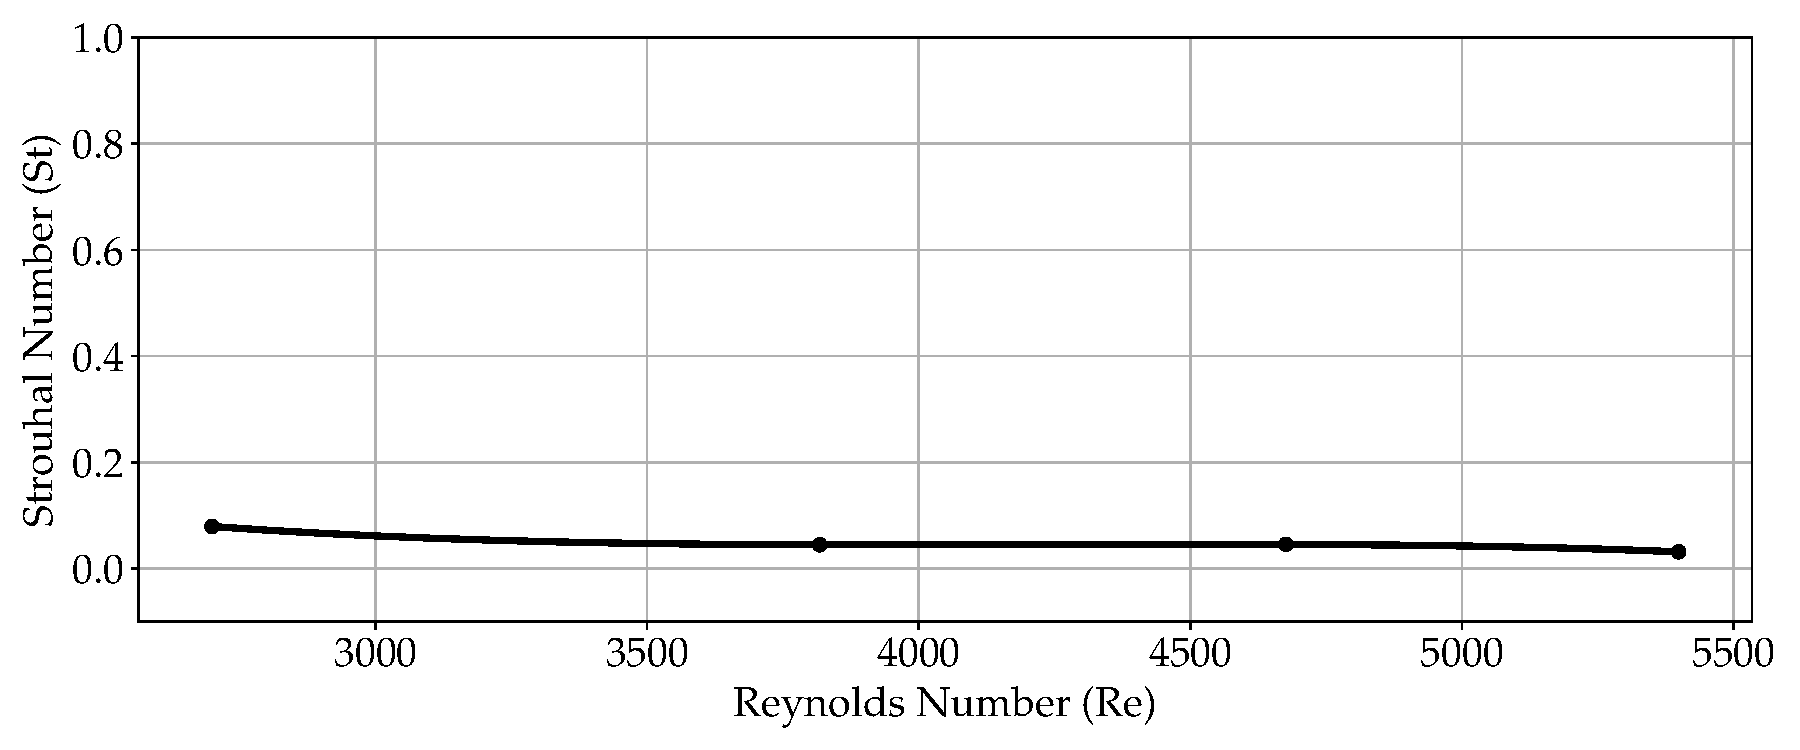
\includegraphics[width=\linewidth]{gfx/Re_vs_St_x_D_y_0.pdf}
    \caption{Variation of Strouhal number ($St$) with Reynolds number ($Re$) for flow past a cylinder at a distance of \enquote{$D$} from the center.}
    \label{fig:st_vs_re_x_D_y_0}
\end{figure}
In the figure, it can be seen that the Strouhal number is decreasing slightly with Reynolds number. This is because the frequency of the vortex decreases with an increase in flow velocity.  The next section discusses the vortex analysis at a distance of $D$ and a height of $0.5~D$ from the center of the cylinder.

\subsection{Vortex analysis at a height of \texorpdfstring{$0.5~D$}~~from the center of the cylinder}

The hot wire anemometer is moved to a height of $0.5~D$ from the center of the cylinder and analysis is performed for four flow speeds having differential pressure of $1~Pa$, $2~Pa$, $3~Pa$ and $4~Pa$. Here, for each flow velocity, the voltage output is measured in the oscilloscope. The corresponding velocity is calculated from the calibration equation (Eq.~(\ref{eq:calib_eqn_hwa})). The velocity is then transformed from the temporal domain to the frequency domain using the Fourier transform equation (Eq.~(\ref{eq:forward fourier})). A comparison of velocity spectral density with frequency for all flow velocities is shown in Fig.~\ref{fig:surface_x_D_y_0-5_D}.
\begin{figure}
    \centering
    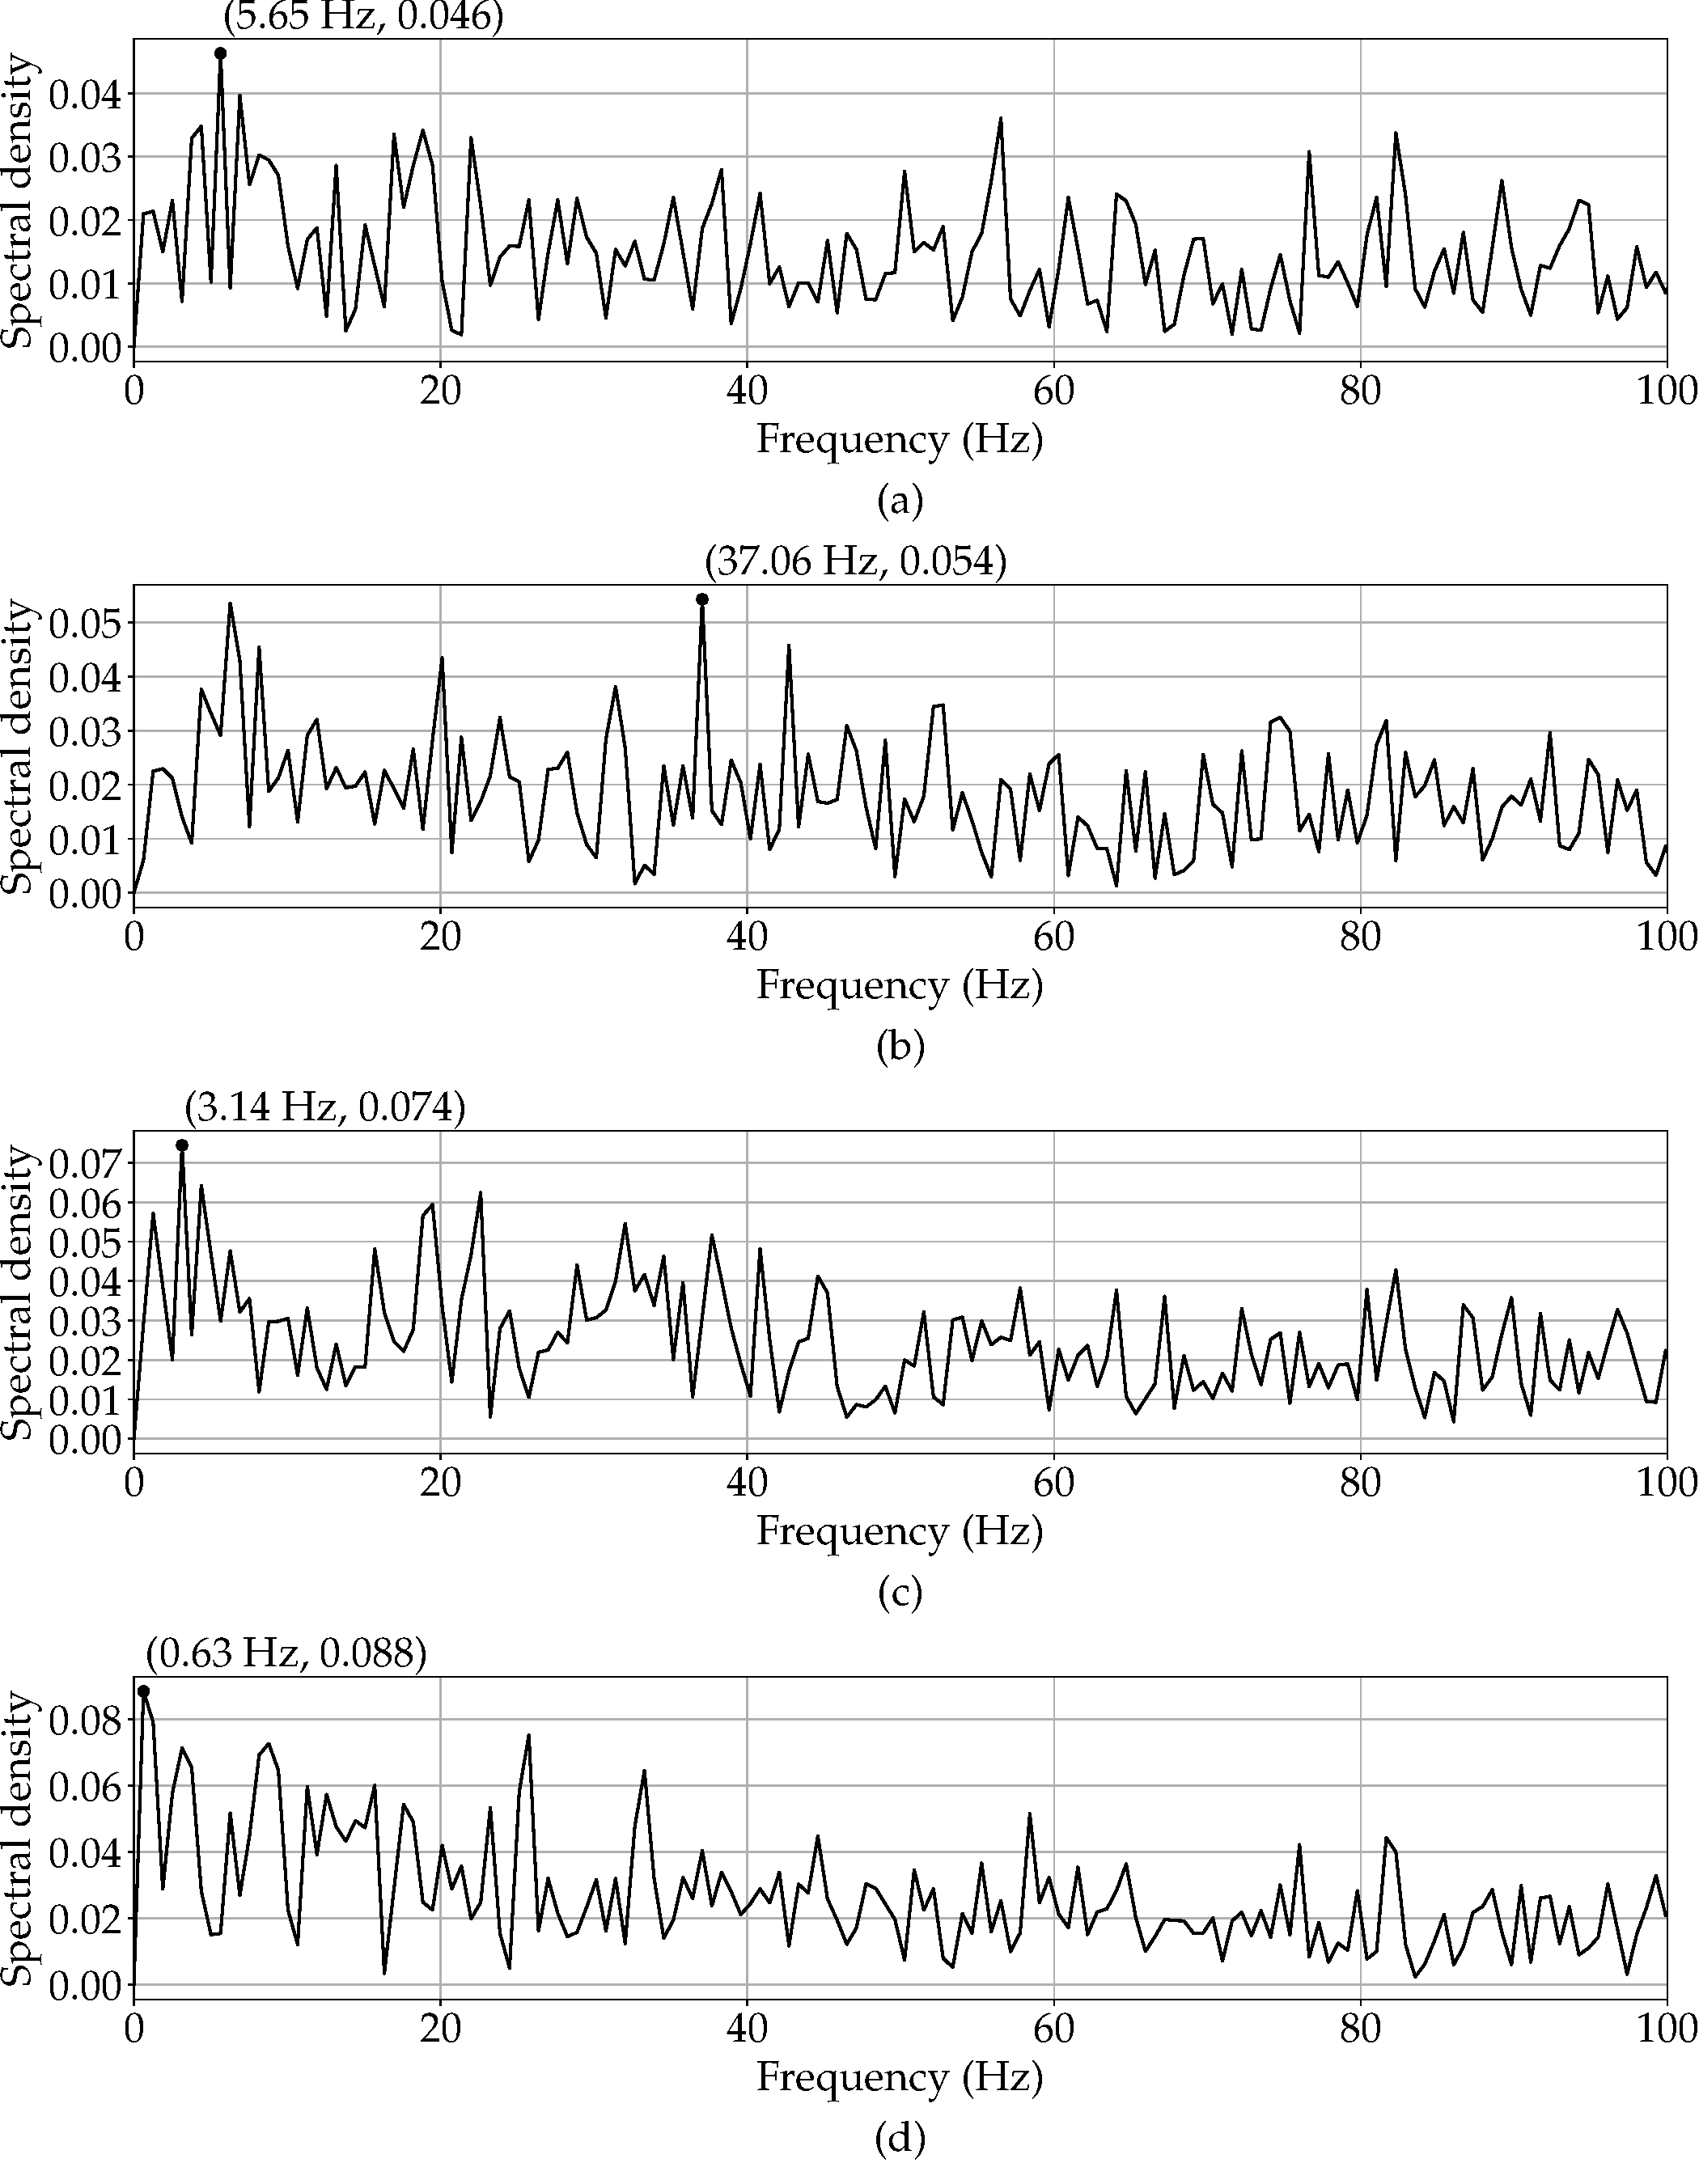
\includegraphics[width=\linewidth]{gfx/FFT_all_freq_x_D_y_0-5_D.pdf}
    \caption{Frequency spectral density of velocity for flow Reynolds number (a)~2699, (b)~3818, (c)~4676 and (d)~5399 at a distance of \enquote{$D$} and a height of \enquote{$0.5~D$} from the center of the cylinder.}
    \label{fig:surface_x_D_y_0-5_D}
\end{figure}
In the figure, it can be seen that the peak frequency for each flow velocity is different from the peak obtained previously. For $Re = 2699$, the peak frequency is 5.65~Hz, for $Re = 3818$, peak frequency is at 37.06~Hz, for $Re = 4676$, the peak frequency is 3.14~Hz and for $Re = 5399$, the peak frequency is 0.63~Hz. These peak frequencies are then used to calculate the Strouhal number (Eq.~(\ref{strouhal number})). The Strouhal number variation with Reynolds number is shown in Fig.~\ref{fig:st_vs_re_x_D_y_0-5_D}. Here, it can be seen that the Strouhal number fluctuates highly in the region of $Re=3000$ to $Re = 4500$. This indicates a change of vortex shedding characteristics when the flow is in transition toward turbulence. The next section discusses the vortex shedding characteristics at a distance of $2~D$ from the center of the cylinder.

\begin{figure}
    \centering
    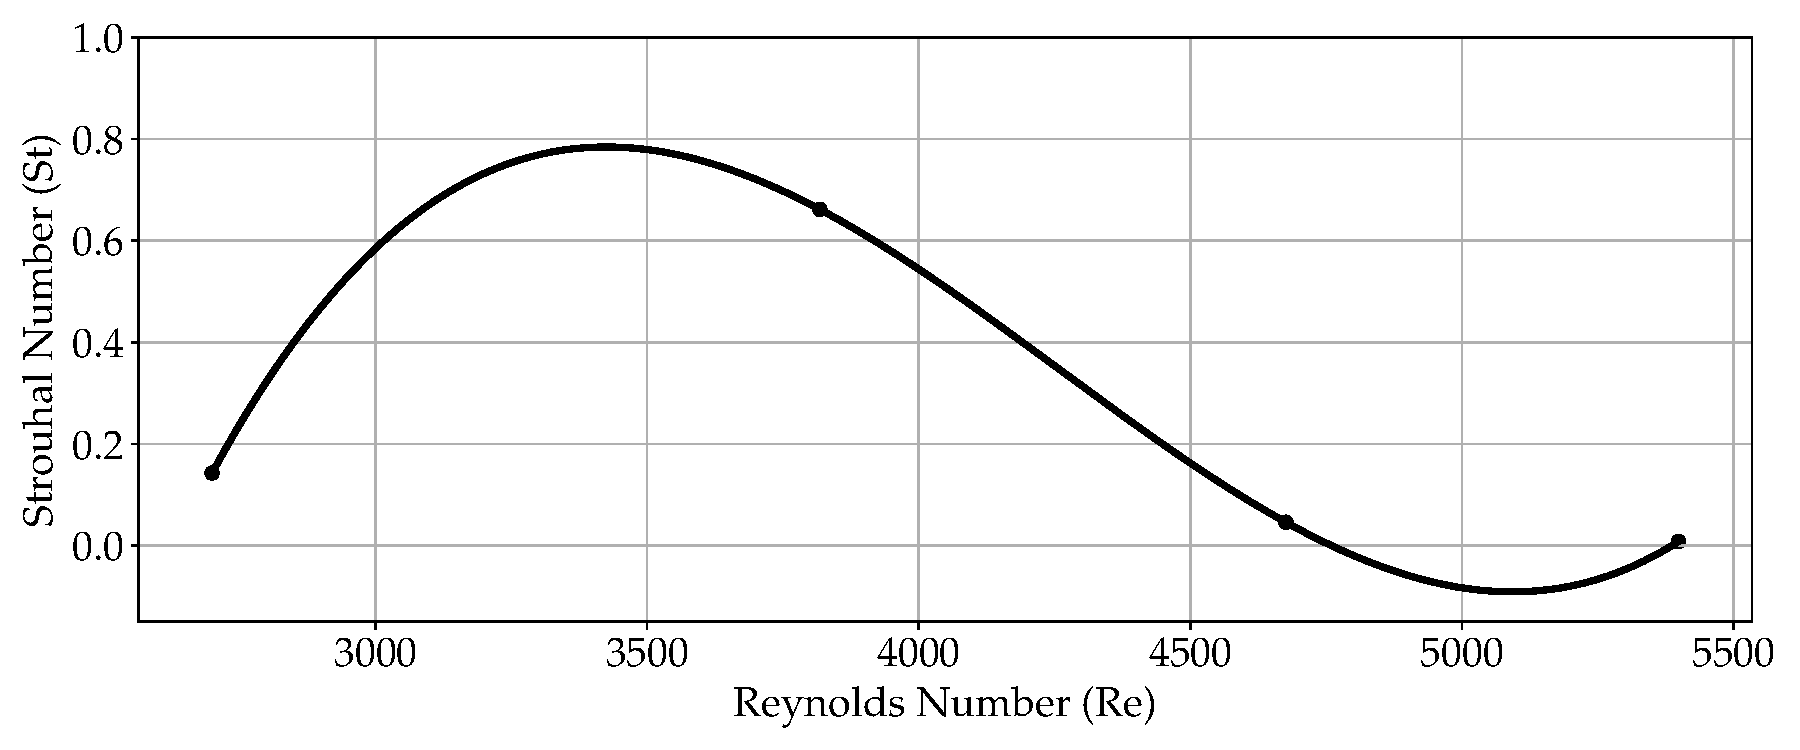
\includegraphics[width=\linewidth]{gfx/Re_vs_St_x_D_y_0-5_D.pdf}
    \caption{Variation of Strouhal number ($St$) with Reynolds number ($Re$) for flow past a cylinder at a distance of \enquote{$D$} and at a height of \enquote{$0.5~D$} from the center of the cylinder.}
    \label{fig:st_vs_re_x_D_y_0-5_D}
\end{figure}

\section{Vortex analysis at distance \texorpdfstring{$x=2D$}~~from the cylinder}
In this section, the vortex shedding characteristics at a distance of $2~D$ from the cylinder is discussed. The analysis is carried out at the center of the cylinder and at a height of $0.5~D$ from the cylinder.
\subsection{Vortex analysis at the center of the cylinder}
The hot wire anemometer is kept at a distance of $2~D$ downstream of the cylinder and the vortices are analyzed for air flow having differential pressures of $1~Pa$, $2~Pa$, $3~Pa$ and $4~Pa$. The output voltage is measured using an oscilloscope and the corresponding velocity is calculated using the calibration equation (Eq.~(\ref{eq:calib_eqn_hwa})). The velocity is transformed from the temporal domain to the frequency domain using Fourier transform (Eq.~(\ref{eq:forward fourier}).  A comparison of velocity spectral density with frequency for all flow velocities is shown in Fig.~\ref{fig:surface_x_2D_y_0}. It can be seen that for $Re = 2699$, the peak frequency is 19.47~Hz, for $Re = 3818$, peak frequency is at 3.77~Hz, for $Re = 4676$, the peak frequency is 0.63~Hz and for $Re = 5399$, the peak frequency is 3.77~Hz. Using these peak frequencies, the Strouhal number is calculated. The variation of the Strouhal number with the Reynolds number is shown in Fig.~\ref{fig:st_vs_re_x_2D_y_0}. 
\begin{figure}
    \centering
    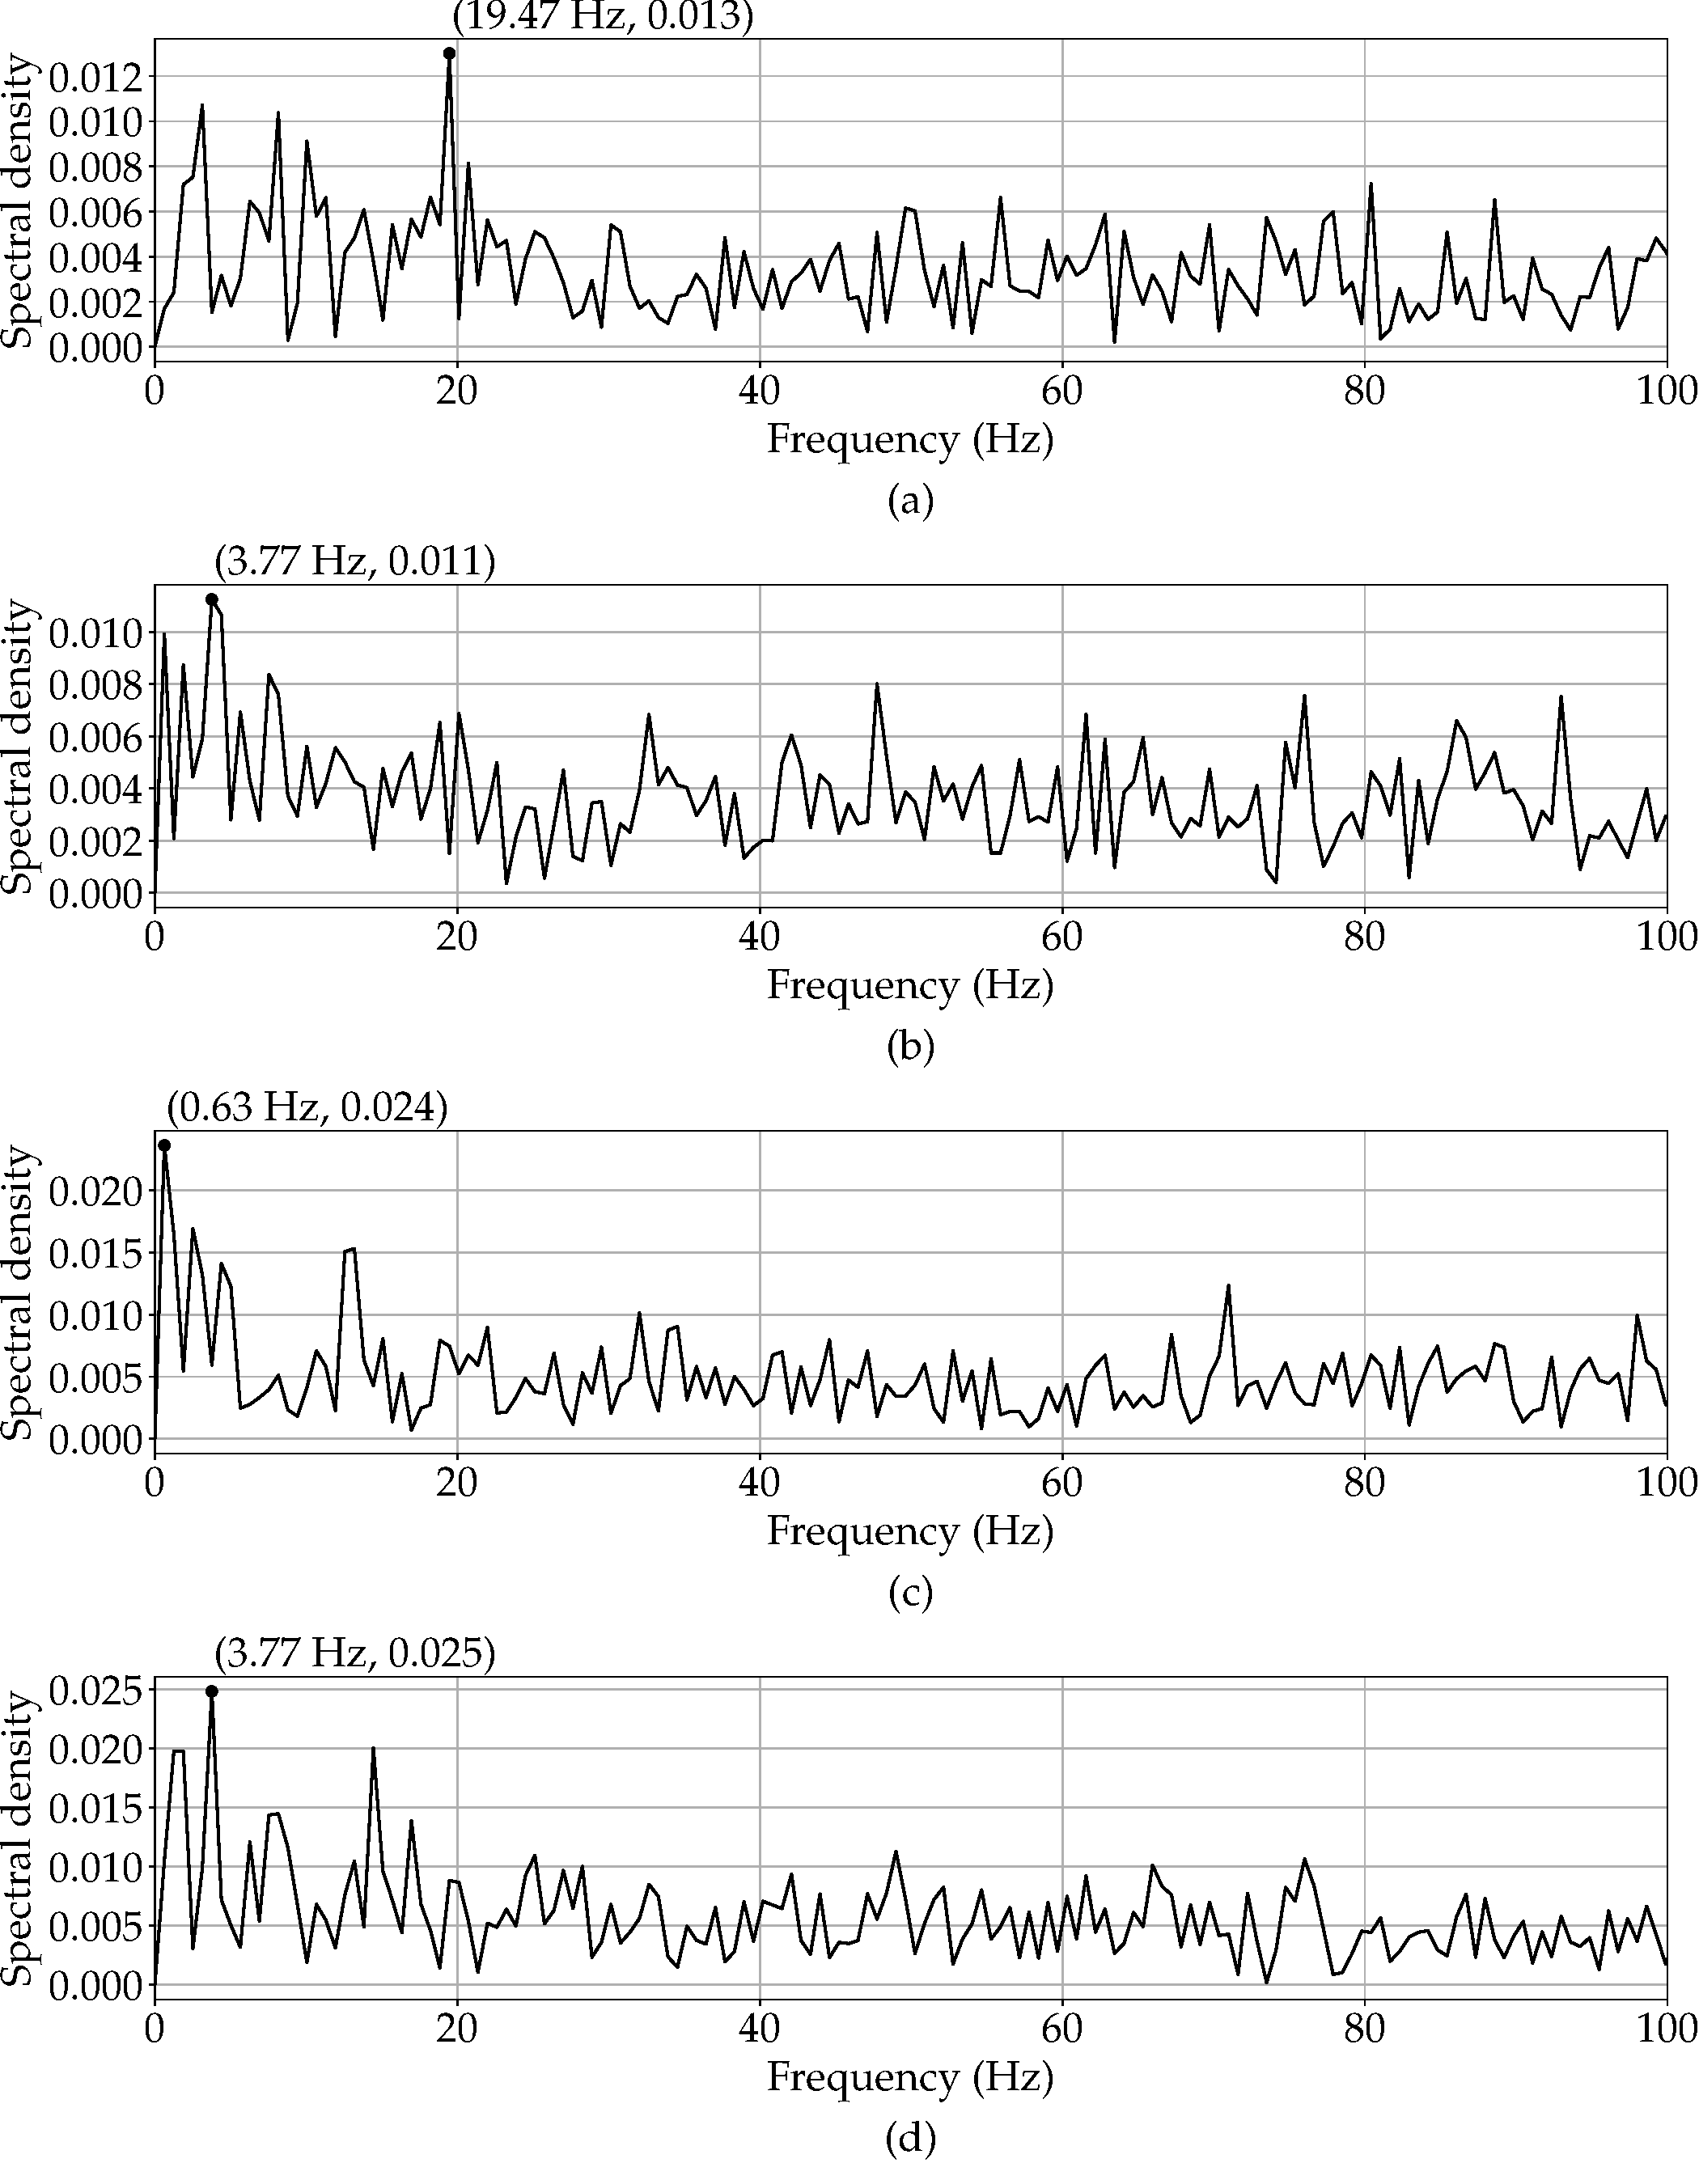
\includegraphics[width=\linewidth]{gfx/FFT_all_freq_x_2D_y_0.pdf}
    \caption{Frequency spectral density of velocity for flow Reynolds number (a)~2699, (b)~3818, (c)~4676 and (d)~5399 at a distance of \enquote{$2~D$} from the center of the cylinder.}
    \label{fig:surface_x_2D_y_0}
\end{figure}

\begin{figure}
    \centering
    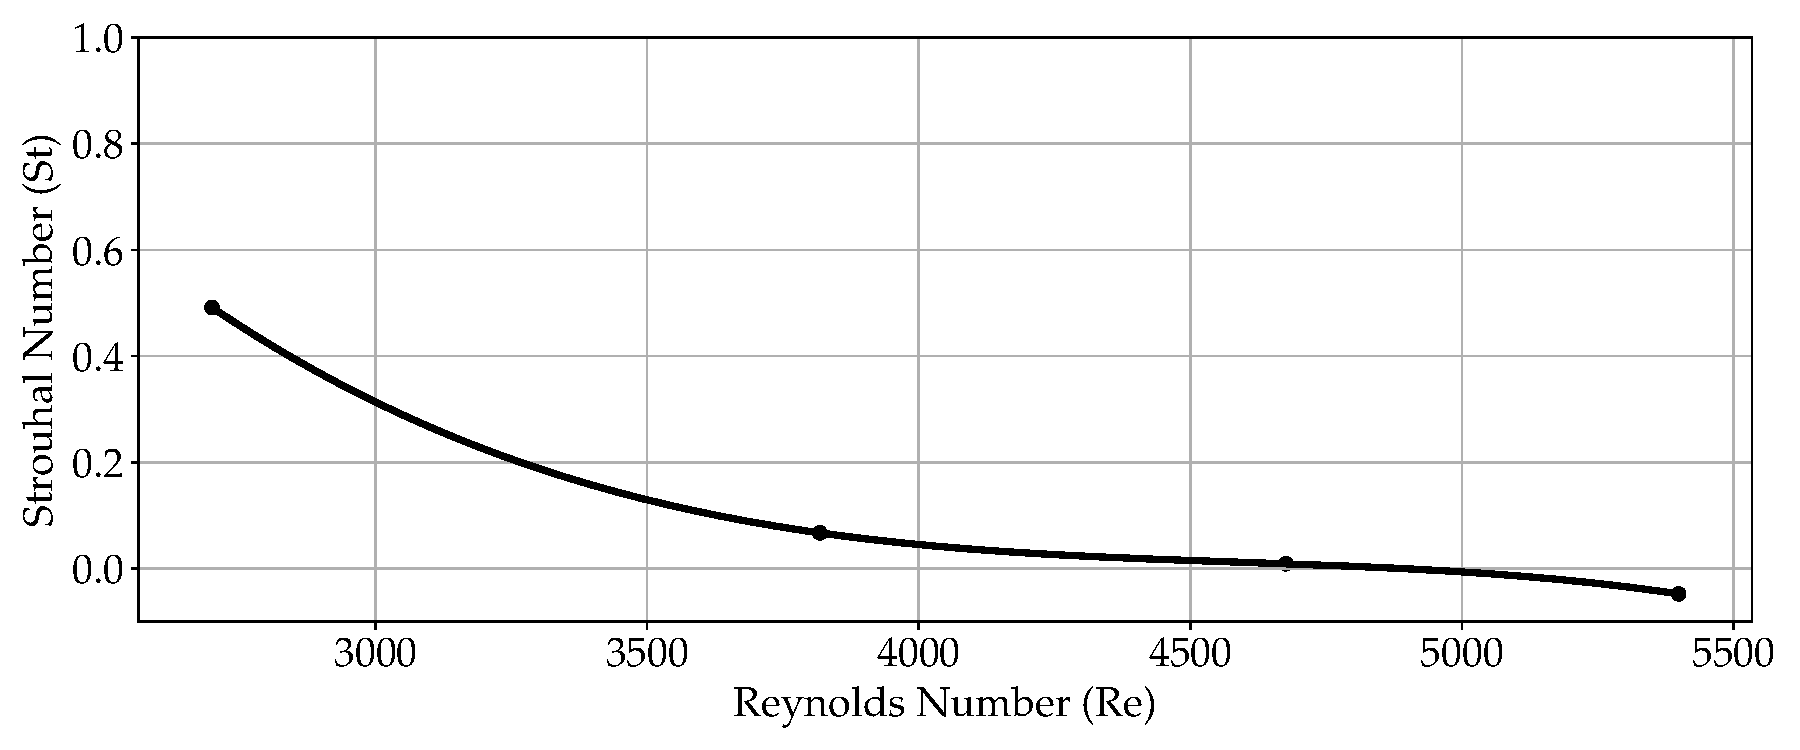
\includegraphics[width=\linewidth]{gfx/Re_vs_St_x_2D_y_0.pdf}
    \caption{Variation of Strouhal number ($St$) with Reynolds number ($Re$) for flow past a cylinder at a distance of \enquote{$2~D$} from the center of the cylinder.}
    \label{fig:st_vs_re_x_2D_y_0}
\end{figure}
In Fig.~\ref{fig:st_vs_re_x_2D_y_0}, it can be seen that the Strouhal number decreases with an increase in the Reynolds number. This is because of the reduction of the frequency of vortices with increase in velocity.

\subsection{Vortex analysis at a height of \texorpdfstring{$0.5~D$}~~from the center of the cylinder}

The hot wire anemometer is then moved to a height of $0.5~D$ from the center of the cylinder and the analysis is performed again for the four flow speeds with differential pressures of $1~Pa$, $2~Pa$, $3~Pa$ and $4~Pa$. For each flow velocity, the voltage output from the hot wire anemometer is measured in the oscilloscope. The velocities corresponding to the voltages are calculated from the calibration equation (Eq.~(\ref{eq:calib_eqn_hwa})). Then it is transformed from the temporal domain to the frequency domain using the Fourier transform equation (Eq.~(\ref{eq:forward fourier})). A comparison of velocity spectral density with frequency for all flow velocities is shown in Fig.~\ref{fig:surface_x_2D_y_0-5_D}.

\begin{figure}
    \centering
    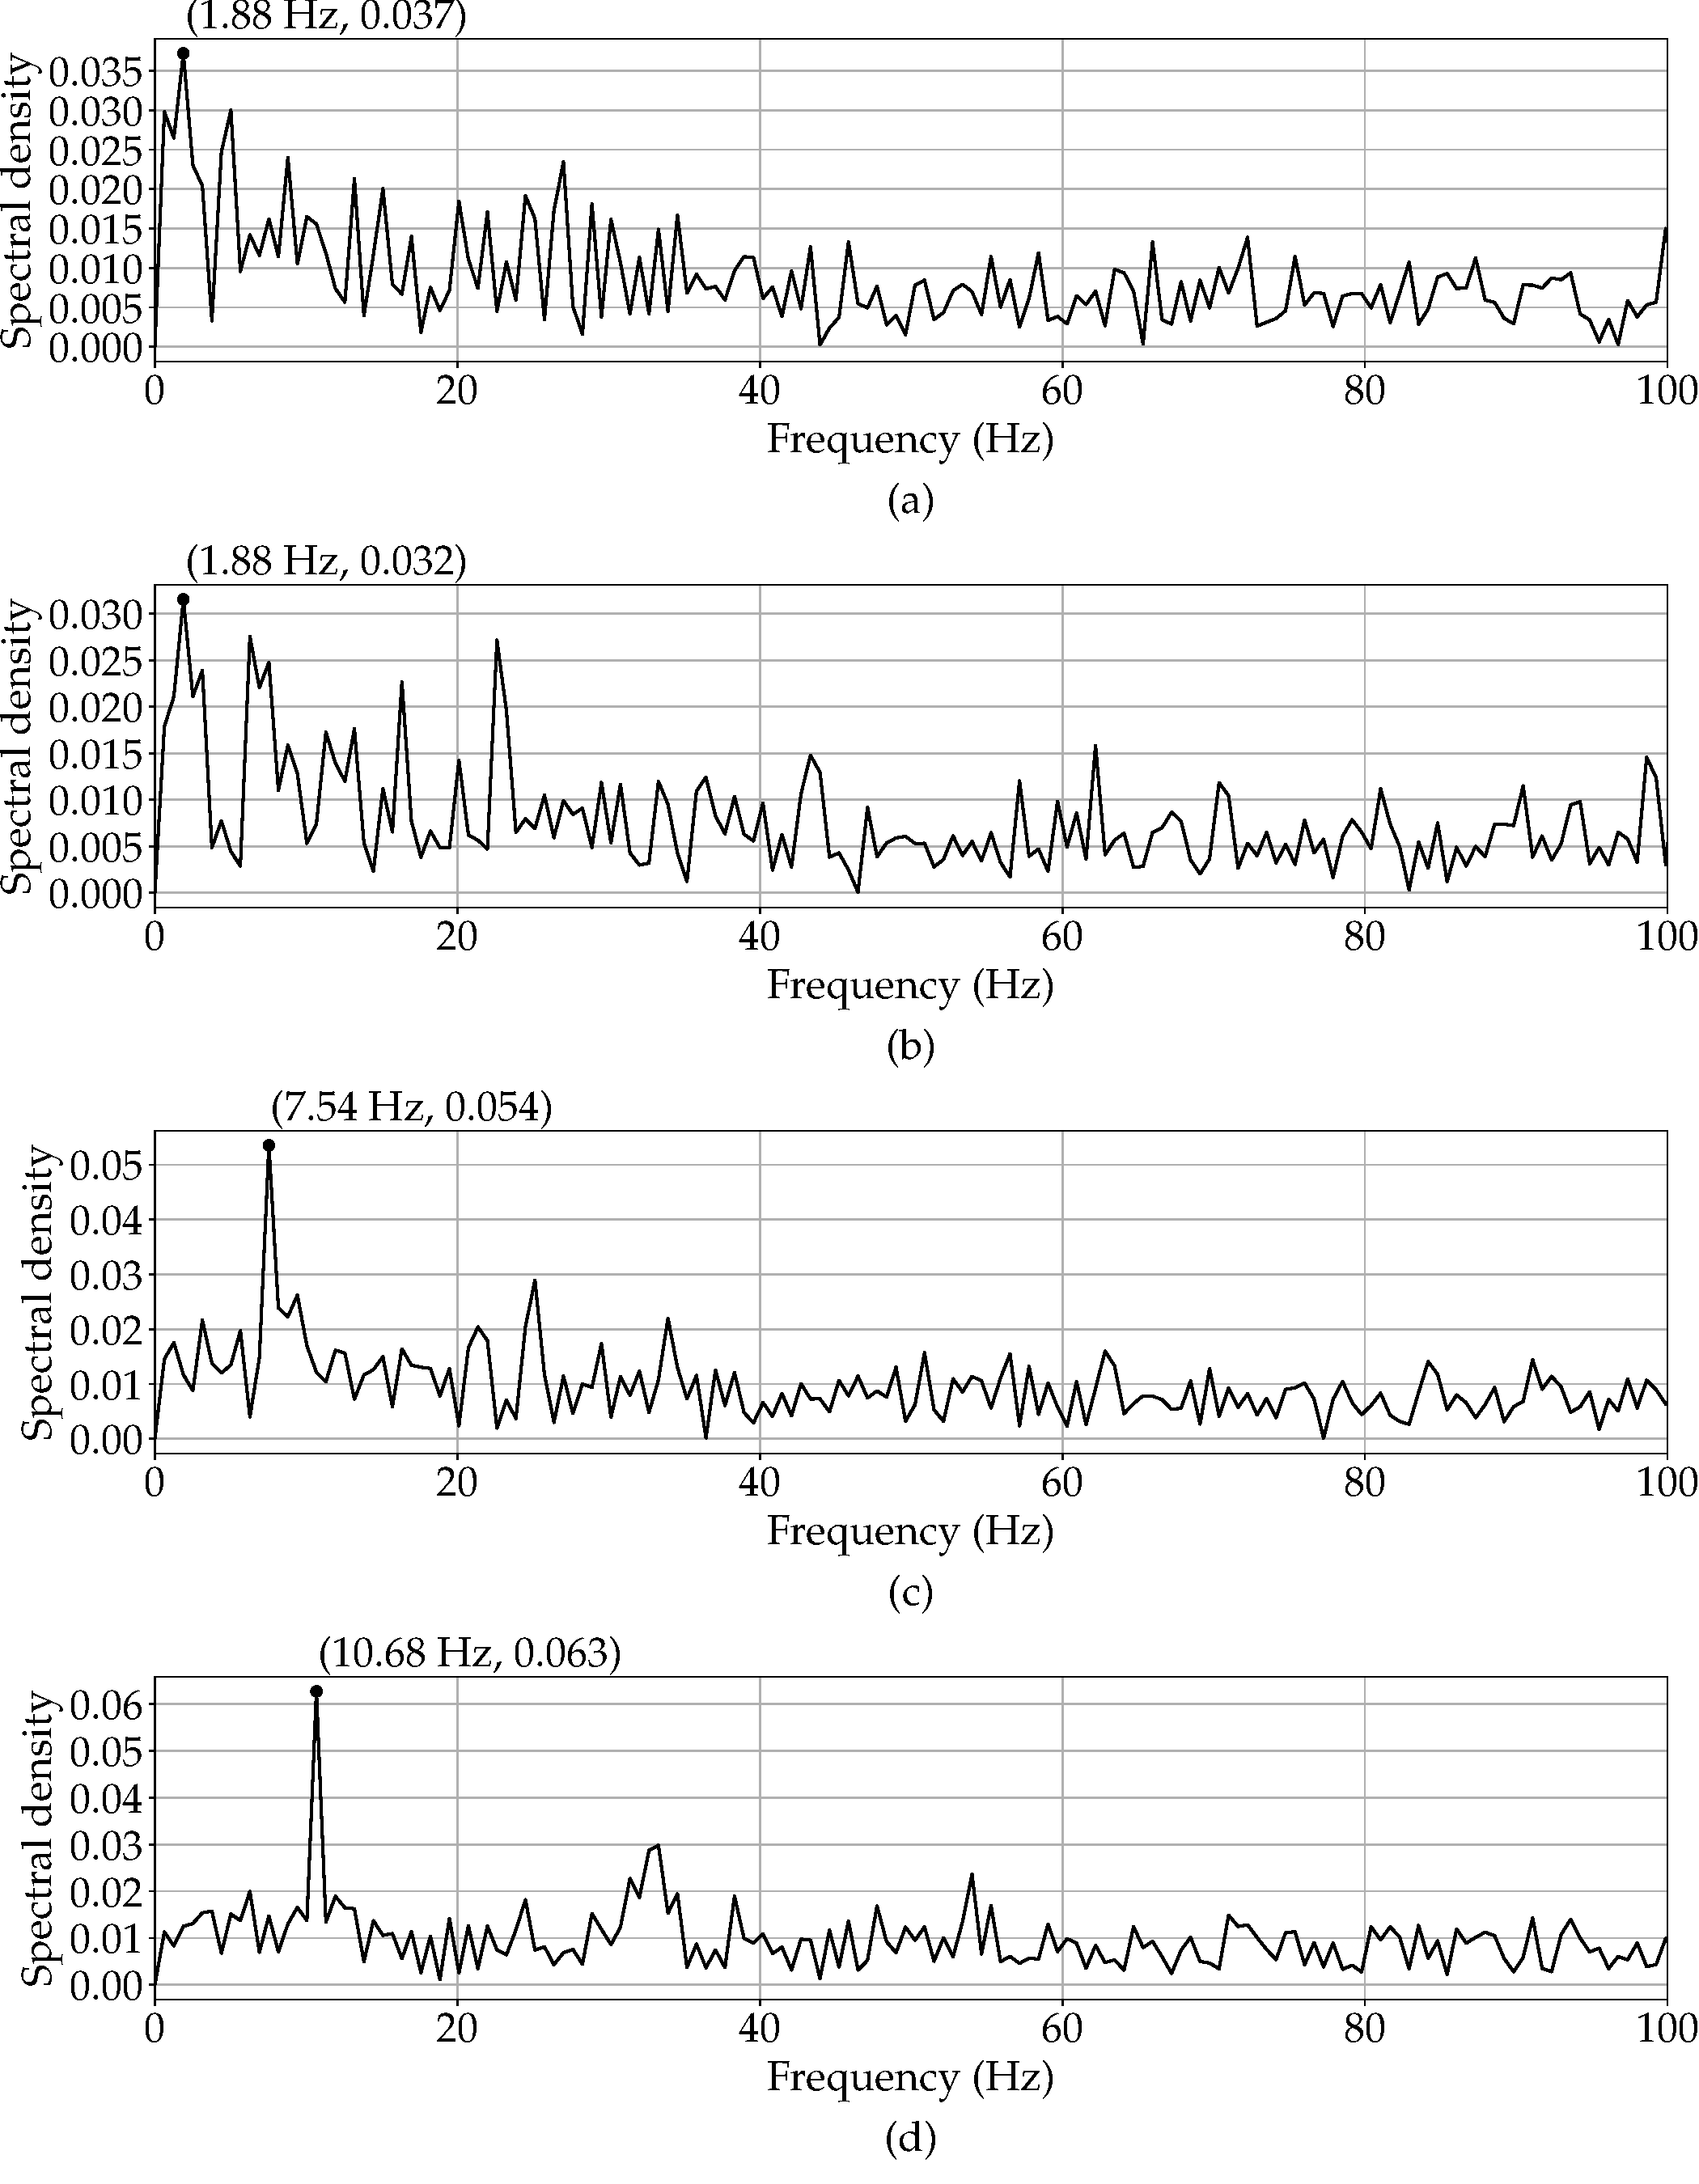
\includegraphics[width=\linewidth]{gfx/FFT_all_freq_x_2D_y_0-5_D.pdf}
    \caption{Frequency spectral density of velocity for flow Reynolds number (a)~2699, (b)~3818, (c)~4676 and (d)~5399 at a distance of \enquote{2~D} and a height of \enquote{0.5~D} from the center of the cylinder.}
    \label{fig:surface_x_2D_y_0-5_D}
\end{figure}

The peak frequencies are 1.88~Hz for $Re = 2699$, 1.88~Hz for $Re = 3818$, 7.54~Hz for $Re = 4676$ and 10.68~Hz for $Re = 5399$. These peak frequencies are used to calculate the Strouhal number (Eq.~(\ref{strouhal number})) and is plotted against the Reynolds number. The comparison between the Reynolds number and the Strouhal number is shown in Fig.~\ref{fig:st_vs_re_x_2D_y_0-5_D}. 
\begin{figure}
    \centering
    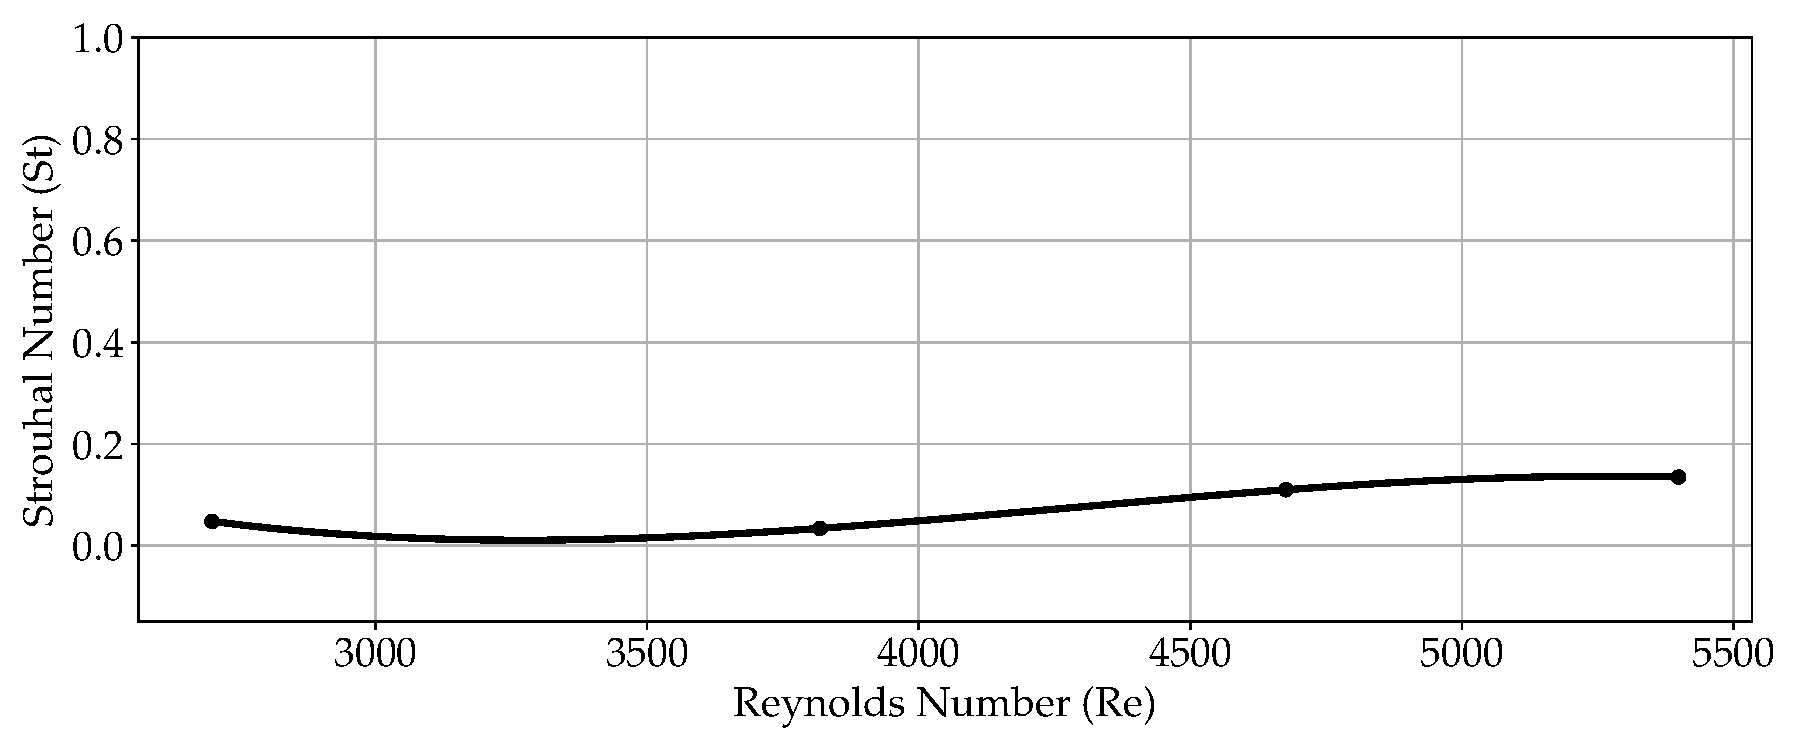
\includegraphics[width=\linewidth]{gfx/Re_vs_St_x_2D_y_0-5_D.pdf}
    \caption{Variation of Strouhal number ($St$) with Reynolds number ($Re$) for flow past a cylinder at a distance of \enquote{$2~D$} and at a height of \enquote{0.5~D} from the center of the cylinder.}
    \label{fig:st_vs_re_x_2D_y_0-5_D}
\end{figure}
Here, the Strouhal number increases with an increase in Reynolds number. This is due to the increase of the vortex frequency when there is an increase in the flow speed. The next section discusses the vortex shedding characteristics at a distance of $4~D$ from the center of the cylinder.

\section{Vortex analysis at distance \texorpdfstring{$x=4D$}~~from the cylinder}
In this section, the vortex analysis is performed at a distance of $4~D$ from the cylinder. The analysis is carried out at the center of the cylinder and at a height of $0.5~D$ from the cylinder.

\subsection{Vortex analysis at the center of the cylinder}
The hot wire anemometer is kept at a distance of $4~D$ downstream of the cylinder and vortex analysis is carried out for air flow having differential pressures of $1~Pa$, $2~Pa$, $3~Pa$ and $4~Pa$. The output voltage across the hot wire anemometer is measured using an oscilloscope and the corresponding velocity is calculated using the calibration equation (Eq.~(\ref{eq:calib_eqn_hwa})). The velocity is transformed from the temporal domain to the frequency domain using Fourier transform (Eq.~(\ref{eq:forward fourier}).  A comparison of velocity spectral density with frequency for all flow velocities is shown in Fig.~\ref{fig:surface_x_4D_y_0}. 
\begin{figure}
    \centering
    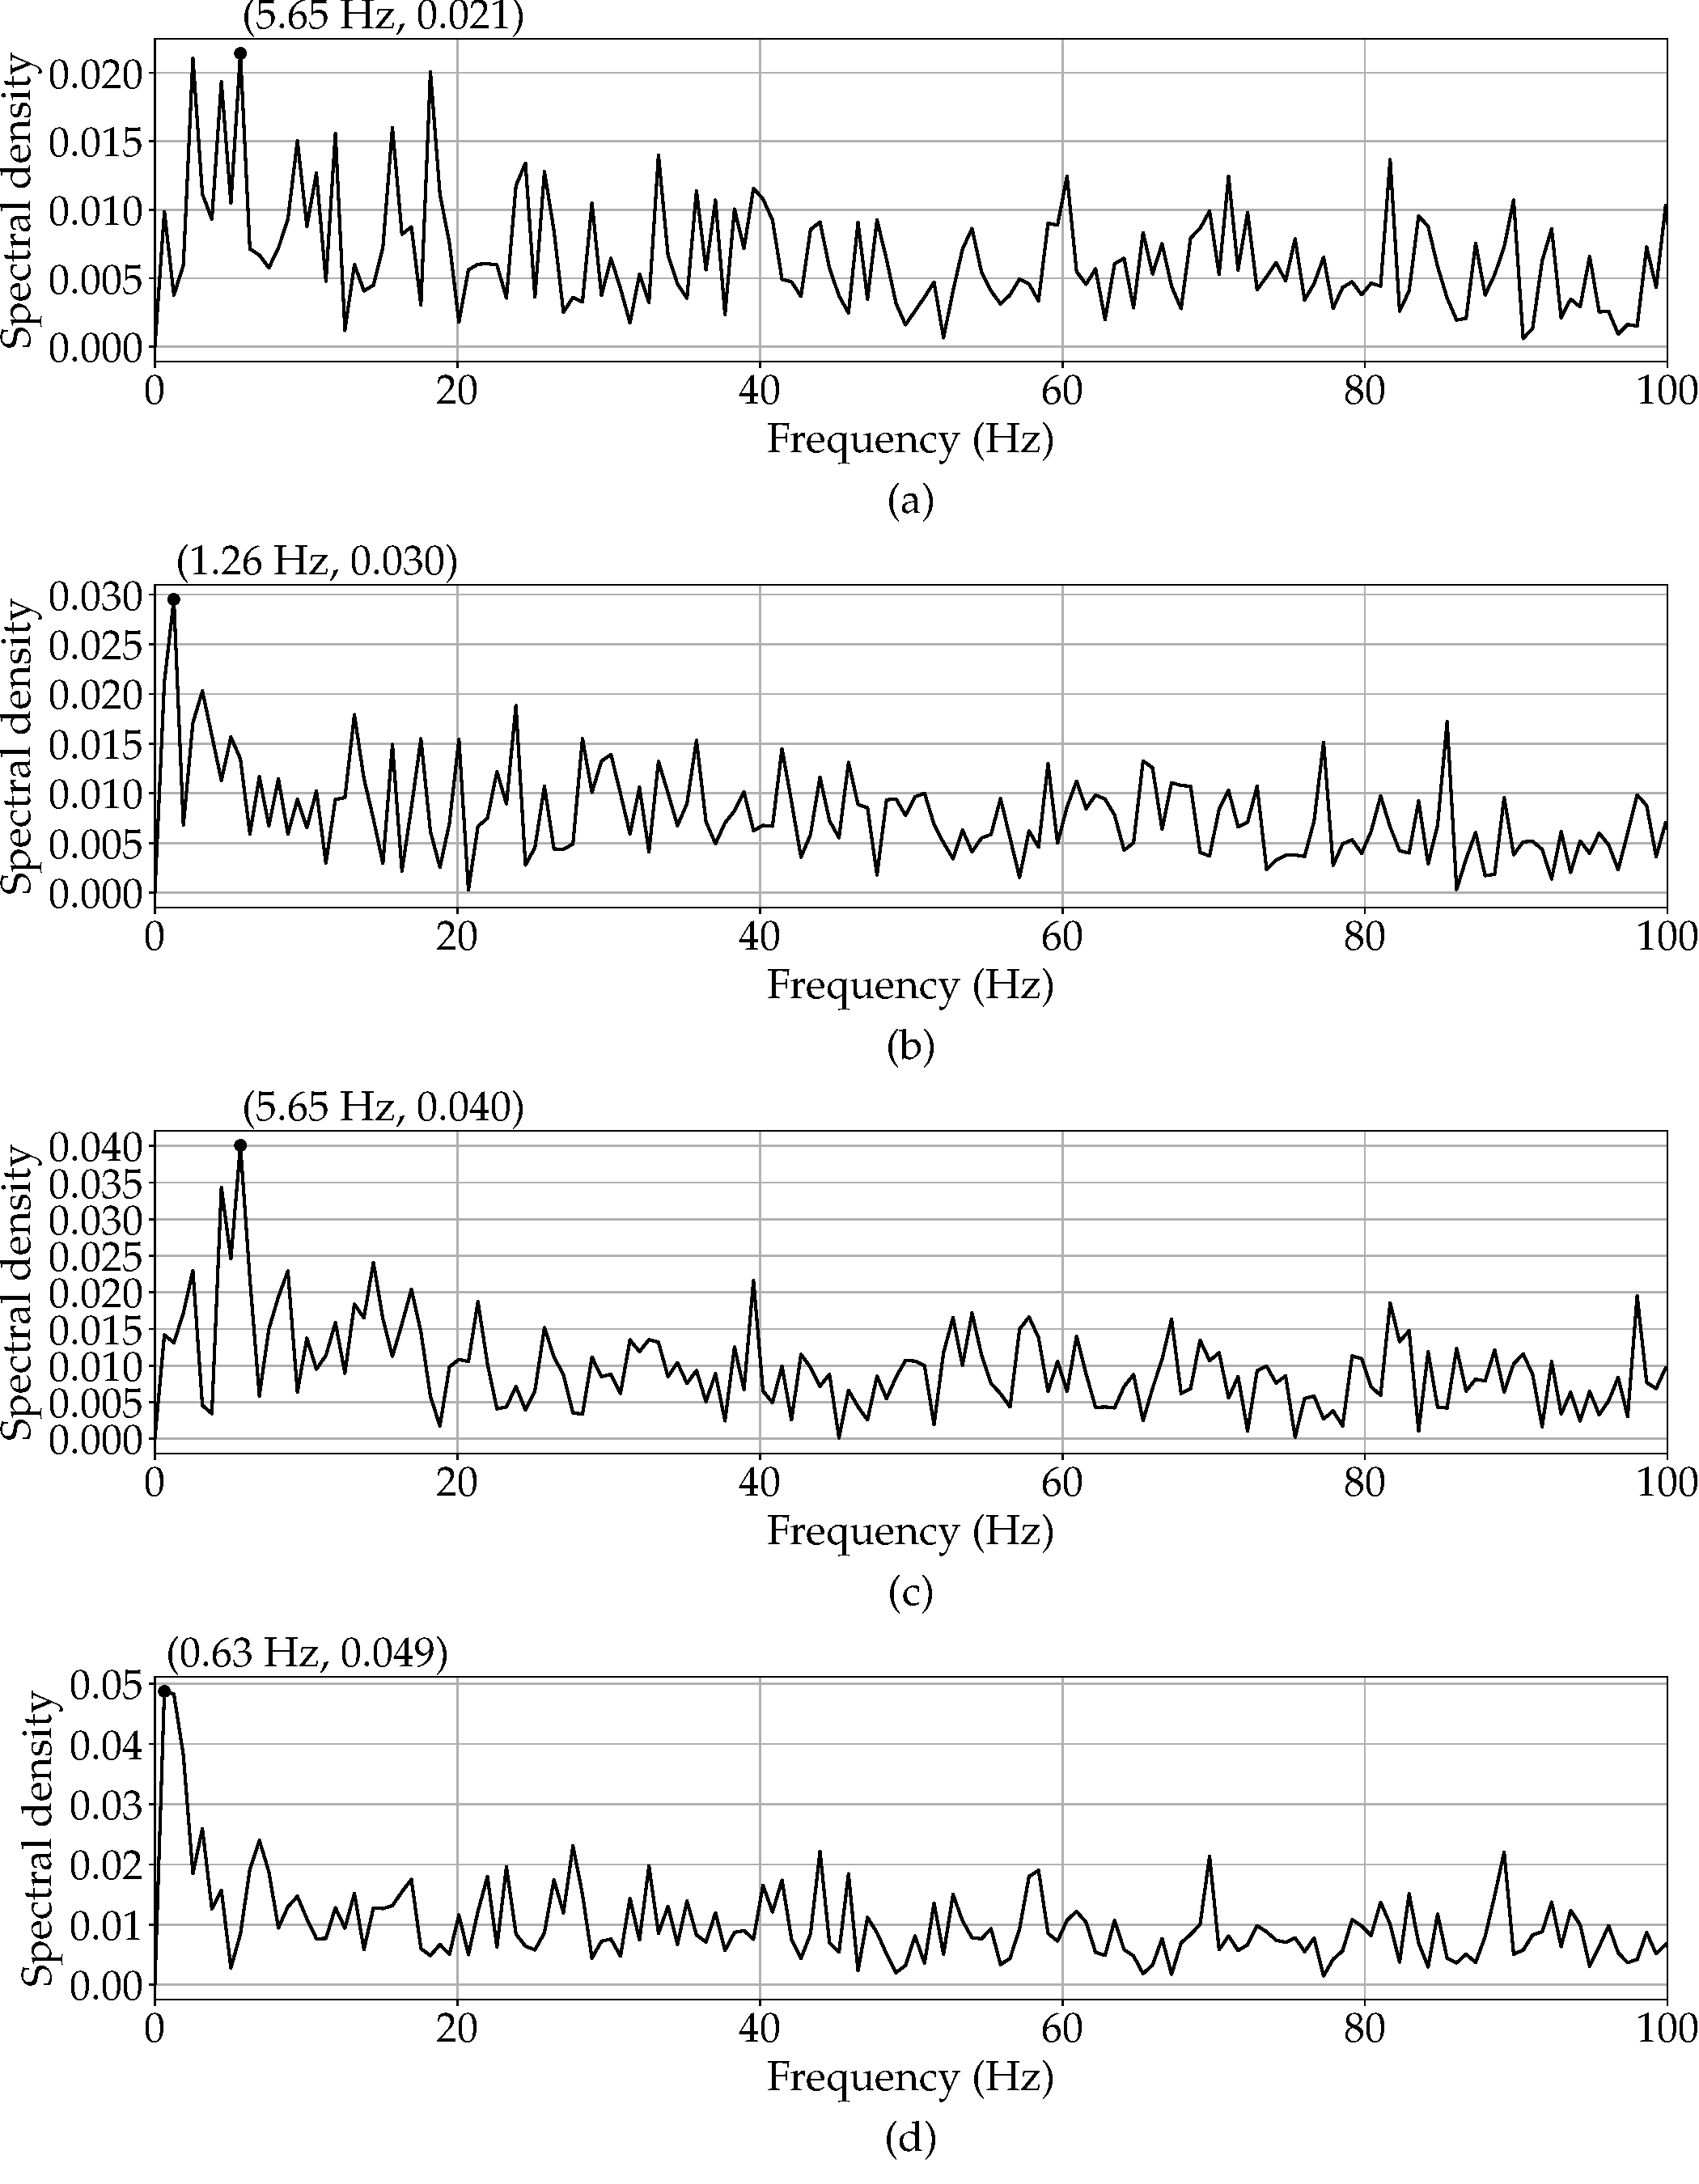
\includegraphics[width=\linewidth]{gfx/FFT_all_freq_x_4D_y_0.pdf}
    \caption{Frequency spectral density of velocity for flow Reynolds number (a)~2699, (b)~3818, (c)~4676 and (d)~5399 at a distance of \enquote{4~D} from the center of the cylinder.}
    \label{fig:surface_x_4D_y_0}
\end{figure}
\begin{figure}
    \centering
    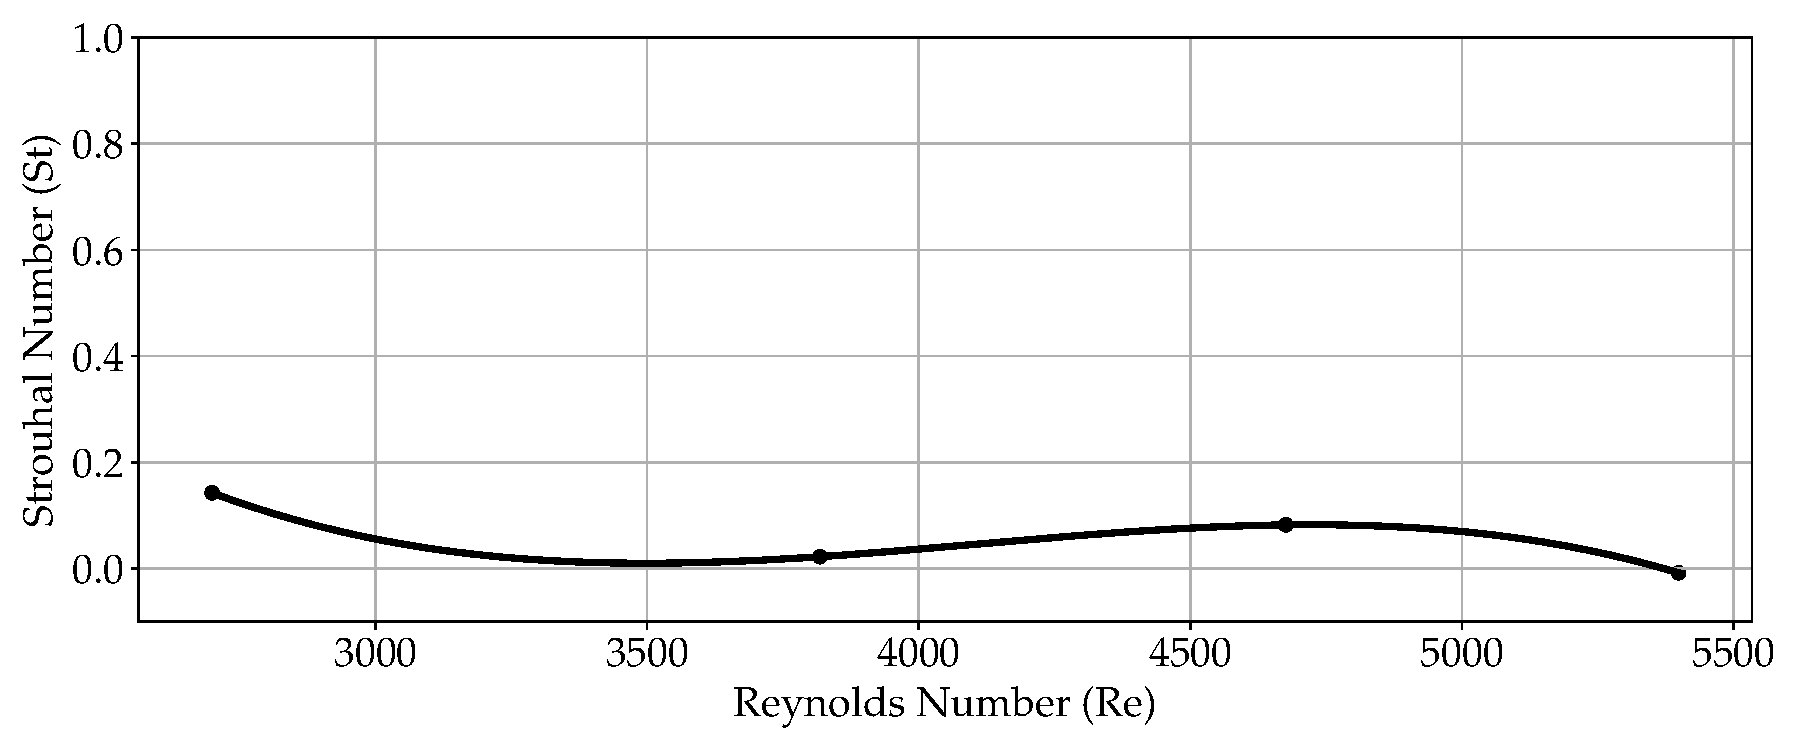
\includegraphics[width=\linewidth]{gfx/Re_vs_St_x_4D_y_0.pdf}
    \caption{Variation of Strouhal number ($St$) with Reynolds number ($Re$) for flow past a cylinder at a distance of \enquote{$4~D$} from the center of the cylinder.}
    \label{fig:st_vs_re_x_4D_y_0}
\end{figure}
It can be seen that for $Re = 2699$, the peak frequency is 5.65~Hz, for $Re = 3818$, peak frequency is at 1.26~Hz, for $Re = 4676$, the peak frequency is 5.65~Hz and for $Re = 5399$, the peak frequency is 0.63~Hz. Using these peak frequencies, the Strouhal number is calculated. The variation of the Strouhal number with the Reynolds number is shown in Fig.~\ref{fig:st_vs_re_x_4D_y_0}. The Strouhal number is in the range 0 to 0.2 which is normal but the low fluctuation is due to its transition towards turbulence.

\subsection{Vortex analysis at a height of \texorpdfstring{$0.5~D$}~~from the center of the cylinder}

The hot wire anemometer is shifted to a height of 0.5~D from the center of the cylinder and vortex analysis is performed for all tow speeds. The voltage output is measured across the sensor in the oscilloscope. The corresponding velocity is calculated from the calibration equation (Eq.~(\ref{eq:calib_eqn_hwa})). The velocity is then transformed from the temporal domain to the frequency domain using the Fourier transform equation (Eq.~(\ref{eq:forward fourier})). A comparison of velocity spectral density with frequency for all flow velocities is shown in Fig.~\ref{fig:surface_x_4D_y_0-5_D}. It can be seen in Fig.~\ref{fig:surface_x_4D_y_0-5_D} that the peak frequencies are 1.26~Hz for $Re = 2699$, 1.26~Hz for $Re = 3818$, 1025.79~Hz for $Re = 4676$ and 1282.71~Hz for $Re = 5399$. The high increase in frequency is due to increased disturbances as the flow is in transition to turbulence. These peak frequencies are used to calculate the Strouhal number (Eq.~(\ref{strouhal number})) and is plotted against the Reynolds number. The comparison between the Reynolds number and the Strouhal number is shown in Fig.~\ref{fig:st_vs_re_x_4D_y_0-5_D}. 
\begin{figure}[H]
    \centering
    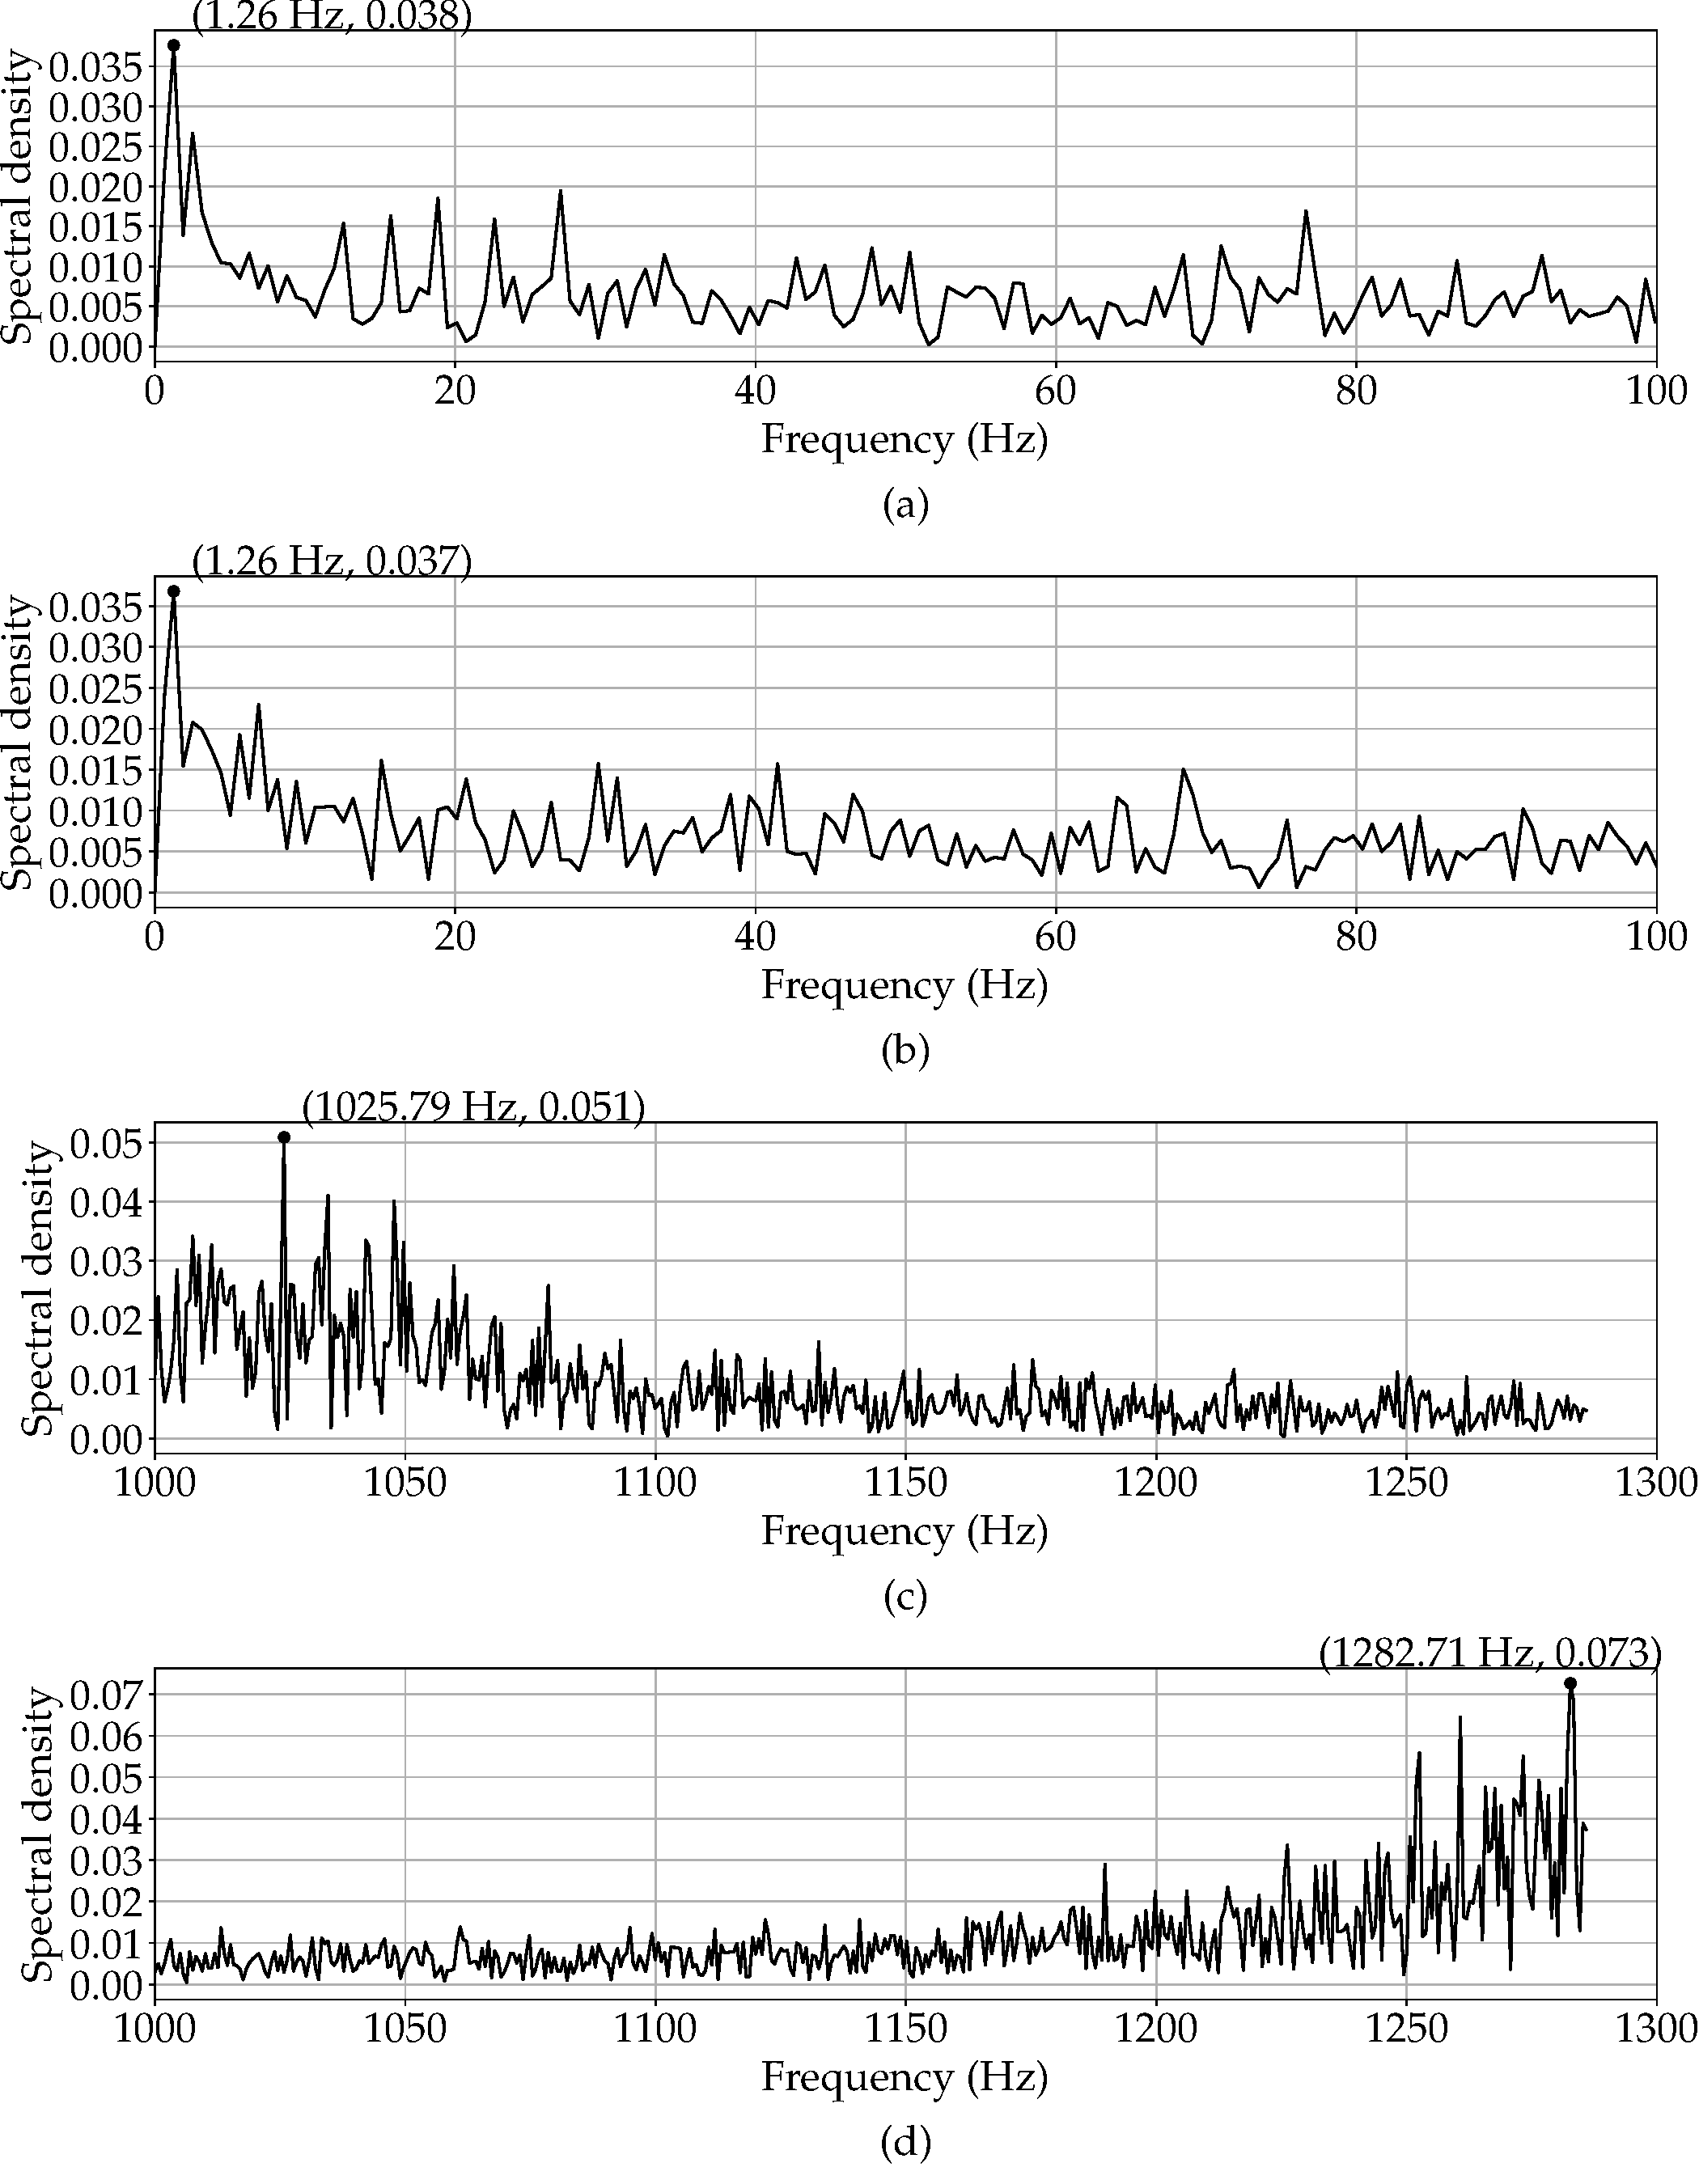
\includegraphics[width=\linewidth]{gfx/FFT_all_freq_x_4D_y_0-5_D.pdf}
    \caption{Frequency spectral density of velocity for flow Reynolds number (a)~2699, (b)~3818, (c)~4676 and (d)~5399 at a distance of \enquote{4~D} and a height of \enquote{0.5~D} from the center of the cylinder.}
    \label{fig:surface_x_4D_y_0-5_D}
\end{figure}
\begin{figure}[H]
    \centering
    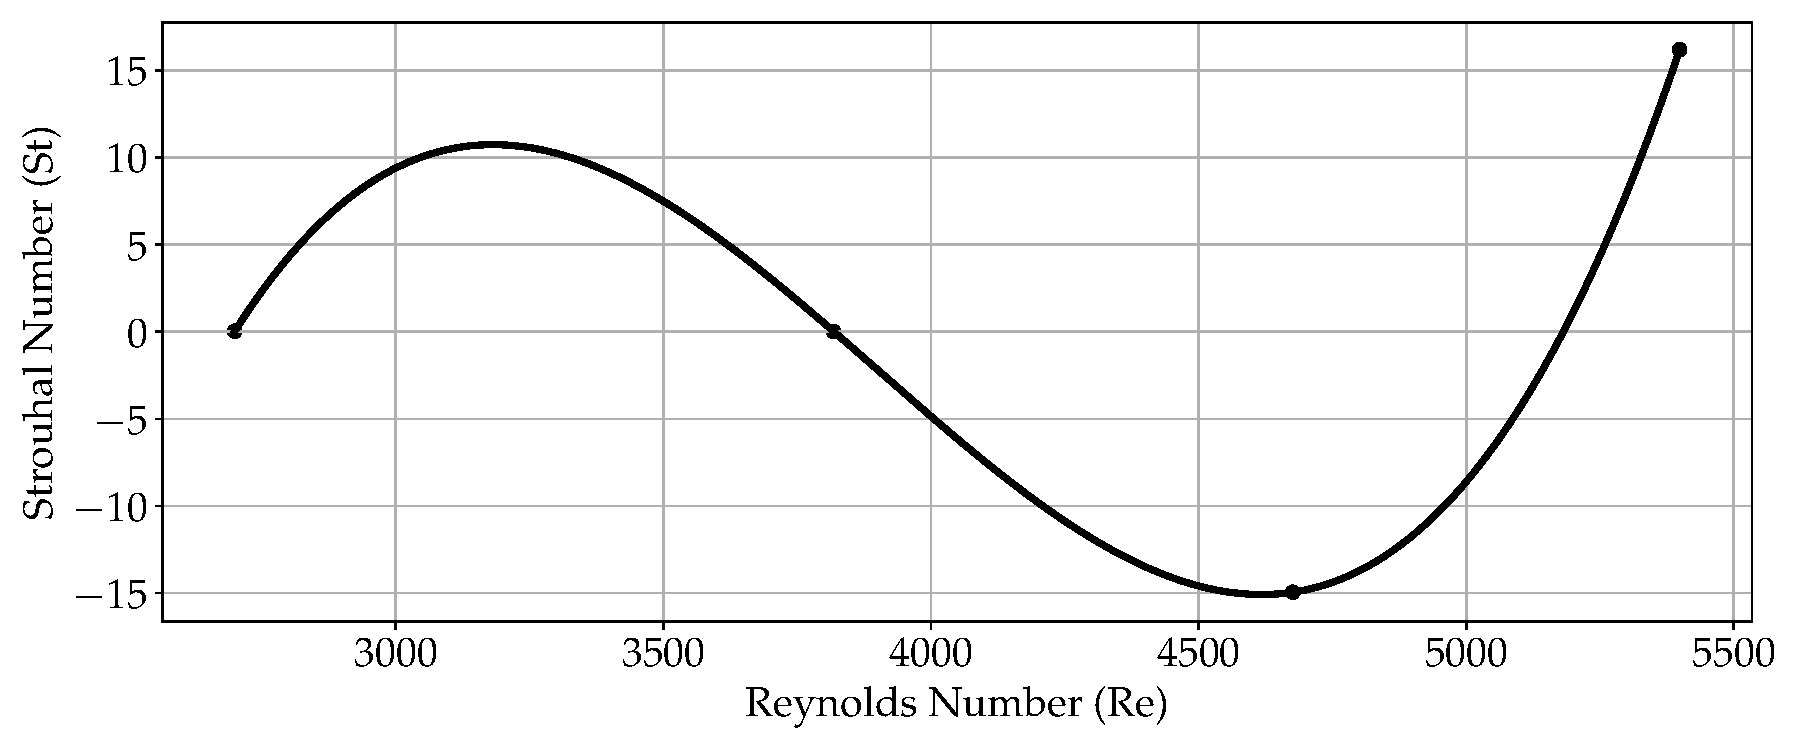
\includegraphics[width=\linewidth]{gfx/Re_vs_St_x_4D_y_0-5_D.pdf}
    \caption{Variation of Strouhal number ($St$) with Reynolds number ($Re$) for flow past a cylinder at a distance of \enquote{$4~D$} and a height of \enquote{$0.5~D$} from the center of the cylinder.}
    \label{fig:st_vs_re_x_4D_y_0-5_D}
\end{figure}

\section{Chapter summary}
In this chapter, the vortex shedding analysis for a flow with differential pressures of $1~Pa$, $2~Pa$, $3~Pa$ and $4~Pa$ is discussed. For this analysis, a hot wire anemometer calibrated using a pitot static tube is used. The vortex shedding behavior is studied at various locations in the test section of the wind tunnel. The solid cylinder with diameter $D = 0.033~m$ is placed at a distance of $0.2~m$ from the left end of the test section. The hot wire anemometer is placed at a distance of $D$, $2~D$ and $4~D$ from the center of the cylinder and at a height of $0.5~D$ from each location. The voltage variation of the sensor is measured and its corresponding velocity variation is calculated using the calibration equation (Eq.~(\ref{eq:calib_eqn_hwa})) in temporal domain. Then it is converted to the frequency domain using the forward Fourier transform equation (Eq.~(\ref{eq:forward fourier})). The peak frequency of the vortex is calculated at each point and the corresponding Strouhal number (Eq.~(\ref{strouhal number})) is calculated. The variation of Strouhal number is plotted with Reynolds number at all six locations. The Strouhal number is found to vary between 0 and 0.2 in some locations, and it is deviating very largely at other locations. This is due to the flow transition from laminar region to turbulence.
\chapter{Conclusion}\label{ch:conclusion}
Add your conclusions here..

%---------------------------- Bibliography -------------------------------

% Please add the contents of the .bbl file that you generate,  or add bibitem entries manually if you like.
% The entries should be in alphabetical order


% ********************************************************************
% Backmatter
%*******************************************************


\appendix
%\renewcommand{\thechapter}{\alph{chapter}}
\cleardoublepage
\part{Appendix}
%********************************************************************
% Appendix
%*******************************************************
% If problems with the headers: get headings in appendix etc. right
%\markboth{\spacedlowsmallcaps{Appendix}}{\spacedlowsmallcaps{Appendix}}
\chapter{Appendix 1}
Appendices if any...
%********************************************************************
% Other Stuff in the Back
%*******************************************************
\cleardoublepage%********************************************************************
% Bibliography
%*******************************************************
% work-around to have small caps also here in the headline
% https://tex.stackexchange.com/questions/188126/wrong-header-in-bibliography-classicthesis
% Thanks to Enrico Gregorio
\defbibheading{bibintoc}[\bibname]{%
  \phantomsection
  \manualmark
  \markboth{\spacedlowsmallcaps{#1}}{\spacedlowsmallcaps{#1}}%
  \addtocontents{toc}{\protect\vspace{\beforebibskip}}%
  \addcontentsline{toc}{chapter}{\tocEntry{#1}}%
  \chapter*{#1}%
}
%\emergencystretch=1em
\printbibliography[heading=bibintoc]

% Old version, will be removed later
% work-around to have small caps also here in the headline
%\manualmark
%\markboth{\spacedlowsmallcaps{\bibname}}{\spacedlowsmallcaps{\bibname}} % work-around to have small caps also
%\phantomsection
%\refstepcounter{dummy}
%\addtocontents{toc}{\protect\vspace{\beforebibskip}} % to have the bib a bit from the rest in the toc
%\addcontentsline{toc}{chapter}{\tocEntry{\bibname}}
%\label{app:bibliography}
%\printbibliography

%**********************************************************************
\end{document}
% ********************************************************************
